%\title{Kandidaatintyö} %!TeX encoding = ISO-8859-1
%\documentclass[12pt,a4paper,english %,twoside,openright %]{tutthesis}
\documentclass[12pt,a4paper,finnish]{tutthesis}
\usepackage{epigraph}
\usepackage{gensymb}

\usepackage{graphicx}
\usepackage{caption}
\usepackage{subcaption}

\usepackage{booktabs}

\usepackage{amssymb}

% Note that you must choose either Finnish or English here and there in this
% file.
% Other options for document class
  % ,twoside,openright   % If printing on both sides (>80 pages)
  % ,twocolumn           % Can be used in lab reports, not in theses

% Ensure the correct Pdf size (not needed in all environments)
\special{papersize=210mm,297mm}


% LaTeX file for BSC/MSc theses and lab reports.
% Requires the class file (=template) tutthesis.cls, tut-logo,
% exampleFig (as pdf or eps) and example_code.c
% Author: Sami Paavilainen (2006)
% Modified: Heikki Huttunen (@tut.fi) 2012-07-31
%           Erno Salminen   (@tut.fi) 2014-08-15
%             - added text snippets from the writing guide
%             - added lots of comments: both tips and alternative styles
%             - added an example table
%             - and so on...
%           ES, 2014-11-03 Disabled 2nd language from Babel, because it
%                          broke the figure and table captions
%           ES, 2015-01-07 Comments and checked the pagination in twoside mode

% More information about Latex basics:
% [Tobias Oetiker, Hubert Partl, Irene Hyna, Elisabeth Schlegl, The
% Not So Short Introduction to LATEX2e, Version 5.03, April 2014, 171
% pages.  Availbale: http://tobi.oetiker.ch/lshort/lshort.pdf]


%-------------------------------------------------------------------------------
% Define your basic information
%-------------------------------------------------------------------------------
\author{Miikka Hevosmaa}
\title{Koeuunnittelun soveltaminen teollisen mittausprosessin analysointiin ja optimointiin: tapaustutkimus}      % primary title (for front page)
%ONGELMA!!! LIIAN PITKÄ, HEITTÄÄ TARKASTAJAN SEURAAVALLE SIVULLE!!!
\titleB{Otsikko suomeksi} % translated title for abstract
\thesistype{Kandidaatintyö} % or Bachelor of Science, Laboratory Report... 
\examiner{Petri Vuoristo} % without title Prof., Dr., MSc or such

% Special trick to use internal macros outside the cls file
% (e.g. \@author). Trick is reversed with \makeatother a bit later.
\makeatletter

%-------------------------------------------------------------------------------
% Define the pdf document properties.  Fill in your own keywords.
%-------------------------------------------------------------------------------
\hypersetup{   
  pdftitle={\@title},
  pdfauthor={\@author},
  pdfkeywords={design of experiments; measurement systems analysis}
}

%-------------------------------------------------------------------------------
%-------------------------------------------------------------------------------
% Put your thesis' main language last
% http://mirrors.ctan.org/macros/latex/required/babel/base/babel.pdf
% !!! 2014-11-03 Second language seems to mess up figure and table
% !!! captions. Do not use it after all (ES)
%%\usepackage[finnish,english]{babel}
\usepackage[finnish]{babel}
%\usepackage[english]{babel}


%-------------------------------------------------------------------------------
%-------------------------------------------------------------------------------
% You can include special packages or define new commands here at the
% beginning. Options are given in brackets and package name is in
% braces:  \usepackage[opt]{pkg_name}

\usepackage[autostyle]{csquotes}

% Option1) for bibliography does not need additional packages.

% Option2b) for bibliography: old way for using Name-year citations
% http://www.ctan.org/tex-archive/macros/latex/contrib/harvard/ 
%\usepackage{harvard}  


% Option3) for bibliography: newer way, esp. for Name-year citations
% http://www.ctan.org/pkg/biblatex
\usepackage[style=authoryear,maxcitenames=2,backend=bibtexu,
  firstinits=true,uniquename=init]{biblatex}
%% Note that option style=numeric works as well
\addbibresource{references.bib}



%-------------------------------------------------------------------------------
%-------------------------------------------------------------------------------
% You can also add your own commands
\newcommand\todo[1]{{\color{red}!!!TODO: #1}} % Remark text in braces appears in red
\newcommand{\angs}{\textsl{\AA}}              % , e.g. slanted symbol for Ångstöm

% Preparatory content ends here
%-------------------------------------------------------------------------------
%-------------------------------------------------------------------------------


\pagenumbering{Roman}
\pagestyle{headings}
\begin{document}



%-------------------------------------------------------------------------------
% Create the title page.
%-------------------------------------------------------------------------------
% First the logo. Check its language.
\thispagestyle{empty}
%\vspace*{-.5cm}\noindent
\vspace*{-1cm}\noindent

\includegraphics[width=8cm]{tty_tut_logo}   % Bilingual logo



% Then lay out the author, title and type to the center of page.
\vspace{6.8cm}
\maketitle
\vspace{6.cm} % modify if thesis title needs many lines

% Last some additional info to the bottom-right corner
\begin{flushright}  
  \begin{minipage}[c]{6.8cm}
    \begin{spacing}{1.0}
      \textsf{Tarkastaja: Prof. \@examiner}\\
      \textsf{Tarkastaja ja aihe hyväksytty}\\ 
      \textsf{xxxxxxx tiedekuntaneuvoston}\\
      \textsf{kokouksessa dd.mm.yyyy}\\
      %\textsf{Examiner: Prof. \@examiner}\\
      %\textsf{Examiner and topic approved by the}\\ 
      %\textsf{Faculty Council of the Faculty of}\\
      %\textsf{xxxx}\\
      %\textsf{on 1st September 2014}\\
    \end{spacing}
  \end{minipage}
\end{flushright}

% Leave the backside of title page empty in twoside mode
\if@twoside
\clearpage
\fi



%-------------------------------------------------------------------------------
%-------------------------------------------------------------------------------
% Use Roman numbering i,ii,iii... for the first pages (abstract, TOC,
% termlist etc)
\pagenumbering{roman} 
\setcounter{page}{0} % Start numbering from zero because command 'chapter*' does page break


% Some fields in abstract are automated, namely those with \@ (author,
% title in the main language, thesis type, examiner).

% Foreign students do not need Fininsh abstract (tiivistelmä). Move
% this before English abstract if thesis is in Finnish. 

% !!! Problems with other language. Disable it (ES, 2014-11-03)
%%\begin{otherlanguage}{finnish} %  Following text in in 2nd language

%-------------------------------------------------------------------------------
\chapter*{Tiivistelmä}         % Asterisk * turns numbering off
%-------------------------------------------------------------------------------

\begin{spacing}{1.0}
         {\bf \textsf{\MakeUppercase{\@author}}}: \@title\\  % or use \@title when thesis is in Finnish
         \textsf{Tampereen teknillinen yliopisto}\\
         \textsf{Diplomityö, xx sivua, x liitesivua}\\ %
         \textsf{xxxkuu 201x}\\
         \textsf{xxx koulutusohjelma}\\
         \textsf{Pääaine: }\\
         \textsf{Tarkastajat:  Prof. \@examiner}\\ % automated, if just 1 examiner
         \textsf{Avainsanat: }\\
\end{spacing}


%The abstract in Finnish. Foreign students do not need this page.

%Suomenkieliseen diplomityöhön kirjoitetaan tiivistelmä sekä suomeksi
%että englanniksi.

%Kandidaatintyön tiivistelmä kirjoitetaan ainoastaan kerran, samalla
%kielellä kuin työ. Kuitenkin myös suomenkielisillä kandidaatintöillä
%pitää olla englanninkielinen otsikko arkistointia varten.

Työssä on tutkittu

%-------------------------------------------------------------------------------

%%\end{otherlanguage} % End on 2nd language part -- (Disabled 2014-11-03)

% !!! Problems with other language. Disable it (ES, 2014-11-03)
%%\begin{otherlanguage}{english} %  Following text in in 2nd language
%\chapter*{Abstract}
%
%\begin{spacing}{1.0}
%         {\bf \textsf{\MakeUppercase{\@author}}}: \@titleB\\   % use \@titleB when thesis is in Finnish
%         \textsf{Tampere University of Technology}\\
%         \textsf{\@thesistype, xx pages, x Appendix pages} \\
%         \textsf{xxxxxx 201x}\\
%         \textsf{Master's Degree Programme in xxx Technology}\\
%         \textsf{Major: }\\
%         \textsf{Examiner: Prof. \@examiner}\\ % 
%         \textsf{Keywords: }\\
%\end{spacing}
%
%
%The abstract is a concise 1-page description of the work: what was the
%problem, what was done, and what are the results. Do not include
%charts or tables in the abstract.
%
%Put the abstract in the primary language of your thesis first and then
%the translation (when that is needed).

%%\end{otherlanguage} % End on 2nd language part -- (Disabled 2014-11-03)

%-------------------------------------------------------------------------------


\makeatother % Make the @ a special symbol again, as \@author and \@title are not neded after this

%-------------------------------------------------------------------------------
%\chapter*{Preface}
\chapter*{Alkusanat}
%-------------------------------------------------------------------------------

%Acknowledgements to those who contributed to the thesis are generally
%presented in the preface. It is not appropriate to criticize anyone in
%the preface, even though the preface will not affect your grade. The
%preface must fit on one page. Add the date, after which you have not
%made any revisions to the text, at the end of the preface.

~ 
% Tilde ~ makes an non-breakable spce in LaTeX. Here it is used to get
% two consecutive paragraph breaks

Tampere, 1.9.2014

~


Teemu Teekkari



%-------------------------------------------------------------------------------
%
% Add the table of contents, optionally also the lists of figures,
% tables and codes.
%

%\renewcommand\contentsname{Table of Contents} % Set English name (otherwise bilingual babel might break this), 2014-09-01
\renewcommand\contentsname{Sisällys}         % Set Finnish name
\setcounter{tocdepth}{3}                      % How many header level are included
\tableofcontents                              % Create TOC

%\renewcommand\listfigurename{List of Figures}  % Set English name (otherwise bilingual babel might break this)
\renewcommand\listfigurename{Kuvaluettelo}    % Set Finnish name
\listoffigures                                 % Optional: create the list of figures
\markboth{}{}                                  % no headers

%\renewcommand\listtablename{List of Tables}    % Set English name (otherwise bilingual babel might break this)
\renewcommand\listtablename{Taulukkoluettelo} % Set Finnish name
\listoftables                                  % Optional: create the list of tables
\markboth{}{}                                  % no headers


%\renewcommand\lstlistlistingname{List of Programs}      % Set English name (otherwise bilingual babel might break this)
%%\renewcommand\lstlistlistingname{Ohjelmaluettelo} % SetFinnish name, remove this if using English
%\lstlistoflistings                                % Optional: create the list of program codes
%\markboth{}{}                                     % no headers


%
% Term and symbol exaplanations use a special list type
%

%-------------------------------------------------------------------------------
\chapter*{Lyhenteet ja merkinnät}
%\chapter*{Lyhenteet ja merkinnät}
\markboth{}{}                                % no headers
%-------------------------------------------------------------------------------

% You don't have to align these with whitespaces, but it makes the
% .tex file more readable
\begin{termlist}
\item [ANOVA]      Analysis of variance, varianssianalyysi
\item [GR\&R] 	   Gauge repeatability and reproducibility study, myös Gage ...
\item [MSA]        Measurement Systems Analysis, mittajärjestelmäanalyysi
\item [RPD]        Robust parameter design, robustien parametrien suunnittelu
\item [RSM]        Response surface methodology, vastepintamenetelmä
\item [SNR]        Signal to noise ratio, signaali-kohinasuhde
\end{termlist} 

\begin{termlist}
\item [$\sigma$] keskihajonta (engl. standard deviation)
\item [$\sigma^2$] varianssi
\end{termlist} 

% The abbreviations and symbols used in the thesis are collected into a
% list in alphabetical order. In addition, they must be explained upon
% first usage in the text.


% Leave the backside of abbreviation list empty in twoside mode
\cleardoublepage

%-------------------------------------------------------------------------------
% The actual text begins here and page numbering changes to 1,2...
\newpage             % needed for page numbering
\pagenumbering{arabic}
\setcounter{page}{1} % Start numbering from zero because command
                     % 'chapter*' does page break
\renewcommand{\chaptername}{} % This disables the prefix 'Chapter' or
                              % 'Luku' in page headers (in 'twoside'
                              % mode)
%-------------------------------------------------------------------------------
\chapter{Johdanto}
\label{ch:johdanto} 
%-------------------------------------------------------------------------------

% \label{...} allows cross-referencing, e.g. 'as explained in
% Chapter~\ref{ch:intro}' Note that you may have to run the command
% 'latex' or 'pdflatex' twice to get cross-references correctly.  You
% can add labels e.g. to chapters, sections, figures, tables, and
% equations.

% You can write everything into single tex file. Alternatively, you
% can write each chapter into separate file and then include them her
% \include{intro} % no postfix .tex to the command
% \include{related_works} % and so on...


%This document template conforms to Guide to Writing a Thesis Tampere
%University of technology (TUT) \cite{thesisguide13}. A thesis or a
%report typically include the following chapters:
%\begin{itemize}
%  \setlength{\itemsep}{-10pt} % Put these lines closer to each other
%\item[] Title page           % Empty bracket[] remove the bullet
%\item[] Abstract
%\item[] Preface
%\item[] Contents
%\item[] List of abbreviations and symbols
%\item[] 1. Introduction
%\item[] 2. Theoretical background
%\item[] 3. Research methodology and materials
%\item[] 4. Results and analysis (possibly split into separate chapters)
%\item[] 5. Conclusions
%\item[] References
%\item[] Appendices (if applicable)
%\end{itemize}


%Introduction outlines the purpose and objectives of the presented
%research. The background information, utilized methods and source
%material are presented next at a level that is necessary to understand
%the rest of the text. Then comes the discussion regarding the achieved
%results, their significance, error sources, deviations from the
%expected results, and the reliability of your research. Conclusions is
%the most important chapter. It does repeat the details already
%presented, but summarizes and them and analyzes their
%consequences. List of references enables your reader to find the cited
%sources.

Kulumiskestävyyden testaus on kriittinen osa uusien pinnoitteiden kehitystä.
Sovelluskohteesta riippuen kulumiskestävyys voi olla jopa kehitystyön tärkein
tavoite. Näin ollen on selvää että testauksen on annettava luotettavia ja
vertailukelpoisia tuloksia. Ei ole tarkoituksenmukaista luottaa mittaus- ja
testauslaitteisiin varauksetta tutkimatta niitten luotettavuutta kriittisesti.


Nykyiset koesuunnittelumenetelmät kehitettiin alun perin


%This document is structured as follows. Chapter~\ref{ch:doe}
%discusses briefly the basics of writing and presentation style
%regarding the text, figures, tables and mathematical
%notations. Chapters~\ref{sec:ref_styles} and \ref{ch:concl} summarize
%the referencing basics and the whole document. There are two example
%appendices as well (Appendix A and B).
% ~\ref{app:A} and \ref{app:B}). Labels do not with \chapter*



%-------------------------------------------------------------------------------
\chapter{Koesuunnittelu}
\label{ch:doe}
%-------------------------------------------------------------------------------

Kokeiden teko on tapa saada tietoa tutkittavasta ilmiöstä. Se on teorian
ohella yksi tieteellisen menetelmän perusteista ja siten siihen onkin
kehittynyt oma erikoistunut teoreettinen runkonsa, joka limittyy matematiikan ja
tilastotieteen kanssa. Alan muodostumiseen ovat suuresti vaikuttaneet mm.
tilastotieteilijät R. A. Fisher (1890-1962) ja George E. P. Box (1919-2013).
Suomeksi tähän alaan viittaa termi koesuunnittelu, joskus kokeensuunnittelu,
englanniksi design of experiments (DOE) tai experimental design.

Koesuunnittelu on osoittautunut tehokkaaksi työkaluksi teollisuudessa; siellä sitä
sovelletaan prosessien
ja systeemien ymmärtämiseen ja hallintaan \parencite{Antony2006} . Se on yksi prosessinhallinnan
ja laadunhallinnan menetelmistä. Esimerkiksi teollisuudessa suosittu laatujohtamisstrategia
Six Sigma käyttää koesuunnittelun menetelmiä, ja Six Sigma on osoittautunut
ainakin jossain määrin
toimivaksi strategiaksi \parencite{Dusharme2001}.

Koesuunnittelu tutkii yleensä prosessia tai systeemiä. Kuvassa \ref{subfig:malli1}
on yksinkertainen malli prosessista. Tutkija haluaa selvittää miten tekijät
\textit{x\textsubscript{1}, x\textsubscript{2},\ldots,x\textsubscript{n}}
vaikuttavat vasteeseen \textit{y}.
Joissain tapauksissa on hyödyllisempää
jakaa tekijät kahteen ryhmään: niihin joita voimme hallita tavallisessa
prosessissa ja niihin joita ei ole mahdollista tai järkevää yrittää
hallita. Jälkimmäisiä on selkeintä kutsua ei-hallittaviksi tekijöiksi
mutta käytössä ovat myös termit häiriötekijä ja kohinatekijä, sillä englanninkieliseksi
termiksi on vakiintunut noise factor.
Niitä merkitään usein
\textit{z\textsubscript{1}, z\textsubscript{2},\ldots,z\textsubscript{n}} kuten
kuvassa \ref{subfig:malli2}.
Vaste \textit{y} on mikä tahansa mitattava ominaisuus joka syntyy prosessin
lopputuloksena ja jota halutaan hallita.
On yleistä nimetä tutkittavat tekijät malliin A, B, C, jne.

\textcite[s.~3]{Montgomery2012} antaa koesuunnittelulle
seuraavat tavoitteet:

\begin{itemize}
\item Vasteeseen \textit{y} eniten vaikuttavien tekijöiden tunnistaminen
\item Merkittävien tekijöiden asettaminen siten, että \textit{y} on mahdollisimman usein
	mahdollisimman lähellä haluttua arvoa
\item Merkittävien tekijöiden asettaminen siten, että \textit{y}:n vaihtelu on pientä
\item Merkittävien hallittavien tekijöiden \textit{x} asettaminen siten, että
	ei-hallittavien tekijöiden \textit{z} vaikutus on mahdollisimman pieni
\end{itemize}

Vaikutusten tutkimiseksi tekijöille valitaan kokeessa käytettävät tasot, so.
tekijöiden arvot. Yleisintä on valita joka tekijälle 2 (matala ja korkea) tai
3 (matala, keskitaso, korkea) tasoa.
Samassa kokeessa eri tekijöillä voi myös olla eri määrä tasoja, esim. 3:lla tekijällä
2 tasoa ja 1:llä tekijällä 3 tasoa. Tällainen koe on
\textit{sekatasosuunnitelma} (huom. tekijän käännös, engl.
mixed-level design).
Tasojen asettaminen rohkeasti mutta
järkevästi normaalin alueen ulkopuolelle johtaa usein informatiivisimpiin
tuloksiin.

%
%\begin{figure}
%  \begin{center}
%    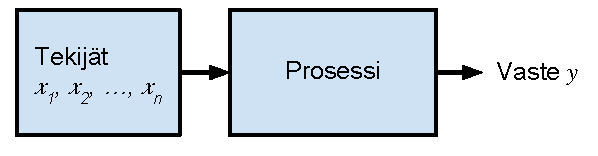
\includegraphics[width=1.0\textwidth]{prosessimalli1}
%  \end{center}
%  \caption[Prosessin yleismalli]{Prosessi ja siihen vaikuttavat tekijät}
%  % Optional shorter caption in brackets is used in Table of Figures
%  % (tof).
%  \label{fig:malli1}
%\end{figure}
%
%\begin{figure}
%  \begin{center}
%    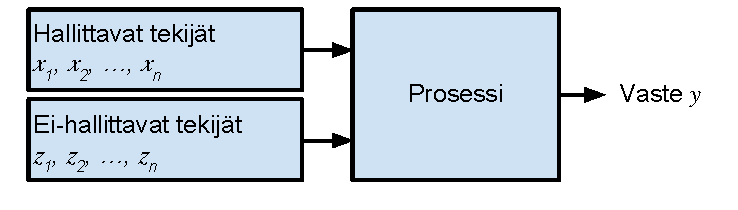
\includegraphics[width=1.0\textwidth]{prosessimalli2}
%  \end{center}
%  \caption[Prosessin vaihtoehtoinen malli]{Tekijät jaettuna hallittaviin ja hallitsemattomiin}
%  % Optional shorter caption in brackets is used in Table of Figures
%  % (tof).
%  \label{fig:malli2}
%\end{figure}
%

\begin{figure*}
  \begin{center}
    \subfigure[Prosessi ja siihen vaikuttavat tekijät.]{
      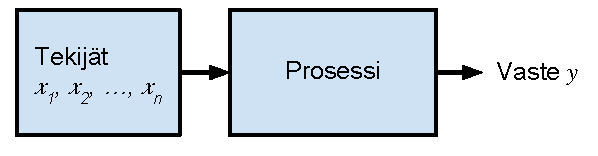
\includegraphics[width=\textwidth]{prosessimalli1}
      \label{subfig:malli1}}
    %\qquad                        % i) Ugly hack to get more horizontal space between figures
    %\hspace{0.05\textwidth}      % ii) Another ugly way to hack space
    % ~~                          % iii) Yet another...

    \subfigure[Prosessin tekijät jaettuna hallittaviin ja ei-hallittaviin.]{
      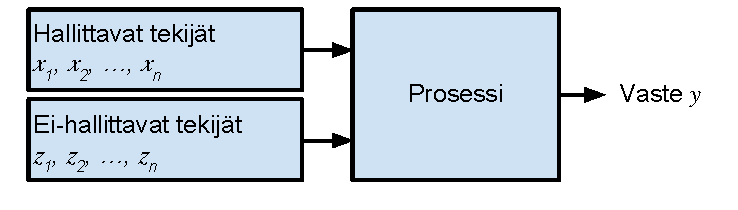
\includegraphics[width=\textwidth]{prosessimalli2}
      \label{subfig:malli2}}
    \caption[Prosessin malleja]{Prosessin malleja. Koesuunnittelussa on joskus
    hyödyllistä jakaa tekijät kuvan mukaisesti.}
    % Optional shorter caption in brackets is used in Table of Figures
    % (tof).

    \label{fig:prosessi}
  \end{center}
\end{figure*}





Opetuksessa usein käytetään esimerkkinä koesuunnittelusta pienoiskatapulttia.
Vasteena on etäisyys joka jää lingotun pallon ja katapultin väliin. Tulokseen
vaikuttaa moni tekijä, joista kokeessa hallitaan esimerkiksi kuminauhojen
kiinnityspisteen korkeutta, laukaisukulmaa, kuminauhojen määrää ja katapultin
varren pituutta. Moni ei-hallittava häiriötekijä
voi myös vaikuttaa tulokseen, esim. satunnaiset ilmavirrat, alustan tasaisuus,
pallon vaihteleva asento katapultin pidikkeessä jne. Hallittaville tekijöille
valitaan tutkittavat tasot, esim. laukaisukulman matalaksi tasoksi voidaan
valita 45 astetta ja korkeaksi 80 astetta ja kuminauhojen määrän matalaksi
tasoksi 1 ja korkeaksi 2. Tavoitteeksi voidaan asettaa esimerkiksi niitten
tekijätasojen löytäminen, joilla pallo lentää mahdollisimman pitkälle,
pallo osuu mahdollisimman lähelle tiettyä etäisyyttä, tai joilla
pallon kulkema etäisyys on aina mahdollisimman lähellä samaa arvoa.


Kokeen tekijä haluaa tietää miten tekijät vaikuttavat lopputulokseen jotta voisi
säätää niitä parhaaksi katsomallaan tavalla. Hän voi ampua katapultilla
useita kertoja vaihdellen
tekijöiden tasoa ja katsoa miten tämä vaikuttaa mittaustulokseen. Koesuunnittelu
tarjoaa työkalut tämän systemaattiseen toteuttamiseen ja tulosten oikeaan
tulkintaan.

Teollisuudessa esiintyy monia samankaltaisia ongelmia. Usein prosessi tuottaa
lopputuotetta jonka mitattava ominaisuus halutaan tietylle tasolle.
Kysymyksiä joihin haetaan vastauksia voivat olla esim: Mitkä tekijät vaikuttavat
tulokseen eniten? Onko tekijöillä yhteisvaikutuksia? Millä tekijöiden yhdistelmällä
lopputulos vaihtelee vähiten? Voiko yhtä tekijää muuttaa (esim. säästötarkoituksessa)
lopputuloksen pysyessä samana jos samalla säädämme muita tekijöitä?
Usein onnistumisessa keskeistä on selkeys ongelman ja halutun ratkaisun
kuvaamisessa ja sekä prosessin että koesuunnittelun asiantuntijoiden tietojen
tehokas käyttö.


Koesuunnitteluun ja muihin tilastollisiin menetelmiin on olemassa monia ohjelmistoja
kuten Minitab, JMP ja Design-Expert. Ohjelmistot auttavat suunnittelussa
mutta menetelmien tunteminen on silti tärkeää jotta vältytään virheiltä
ja vääriltä tulkinnoilta.

\section{Koesuunnitelma}
\label{doe}

Tekijöiden ja tutkittavan vasteen valitsemisen jälkeen on suunniteltava käytettävät
tasot, koeajojen määrä ja tekijätasojen yhdistelmät joilla kokeet ajetaan.
Tuloksena on koesuunnitelma ja se esitetään matriisina jossa rivit ovat
koeajoja ja sarakkeisiin merkitään ajossa käytettävät tekijätasot.
Matala taso merkitään yleensä -1 ja korkea +1, joskus vain - ja +.
Yleistä on myös merkitä tekijän A korkeaa tasoa kirjaimella \textit{a}, tekijän
B korkeaa tasoa kirjaimella \textit{b}, jne. Merkintä \textit{ac} tarkoittaa siis
että
tekijät A ja C ovat korkealla tasolla ja tekijä B matalalla. Esimerkki
suunnitelmamatriisista on taulukko \ref{tab:fullf}.
Kirjallisuudessa esiintyy usein suunnitelman graafinen esitystapa,
"laatikkokuvaaja", kuten kuvassa \ref{fig:cube} \textcite{ehandbook}.
Koe on sama kuin taulukossa \ref{tab:fullf} mutta tekijöitä on
merkitty kirjaimilla \textbf{X\textsubscript{1}}, \textbf{X\textsubscript{2}}
ja \textbf{X\textsubscript{3}}. Nuolet osoittavat tekijän arvon lisäämisen
suunnan ja jokainen kulma on yksi koeajo.

Yksinkertaisinta on muuttaa yhtä tekijää kerrallaan. Koesuunnittelu kuitenkin syntyi
osaksi juuri tarjoamaan vaihtoehtoja tälle hitaalle menetelmälle. On mahdollista luoda
koesuunnitelmia jotka vaativat vähemmän koeajoja kuin yksi tekijä kerrallaan -menetelmä,
ja jotka kuitenkin antavat tietoa myös tekijöiden yhteisvaikutuksista.

Koesuunnitelmia on kehitetty useita erilaisia eri tarkoituksiin.
Suunnitelma on perinteisesti valittu apuna tietämys
tutkinnan kohteesta, tavoitteista ja koesuunnittelumenetelmistä.
Uudempi tapa on luoda tilanteeseen
mukautettu suunnitelma algoritmin ja tietokoneen avulla.

Yhdistely- eli faktorikokeessa (engl. factorial experiment/design) tekijöiden
tasoja vaihdellaan sekä yksitellen että yhdessä. Jos kaikki tasoyhdistelmät
toteutetaan, on kyseessä täysyhdistelykoe (engl.
full factorial design). Tällainen koe arvioi kaikkien tekijöiden kaikki yksittäis-
ja yhdistelmävaikutukset vasteeseen. Kattavuuden hintana on koeajojen
eksponentiaalisesti kasvava määrä kun tekijöitä lisätään kokeeseen: jos kaikilla
tekijöillä on 2 tasoa, on koeajojen määrä \(2^k\),
missä \textit{k} on
tekijöiden lukumäärä. Ko. kokeelle käytetäänkin yksinkertaisesti
merkintää \(2^k\)-koe.
Jos tekijöitä tiedetään olevan 2, merkintä on
\(2^2\) ja niin edelleen. Vastaavasti jos tekijöille on valittu 3 tasoa,
kutsutaan tätä \(3^k\)-kokeeksi, ja jos valittuja tasoja on \textit{I},
niin kutsutaan sitä \(I^k\)-kokeeksi.

Tekijän vaikutusta voidaan arvioida yksinkertaisesti laskemalla vasteen keskiarvo
ensin kaikista tuloksista tekijän ollessa matalalla tasollaan ja sen jälkeen
vasteen keskiarvo tekijän ollessa korkealla tasollaan ja sen jälkeen
vertailemalla niitä keskenään. Kun koesuunnitelma sallii tällaisen matemaattisesti
riippumattoman tarkastelun joka tekijän vaikutuksista, sanotaan
sen olevan \em ortogonaalinen.\em Toisin sanoen matemaattisessa
tarkastelussa koesuunnitelman joka sarakkeen (eli tekijän) välinen kovarianssi
on nolla \parencite{barker2005}.



\begin{table}[h]
  \begin{center}
  \caption{Esimerkki täysyhdistelykokeesta kolmella tekijällä.}
  \label{tab:fullf}
  \begin{tabular}{ | l | c | c | c | }
    \hline
     & \textbf{A} & \textbf{B} & \textbf{C} \\ \hline
    1 & $-$ & $-$ & $-$\\ \hline
    2 & + & $-$ & $-$\\ \hline
    3 & $-$ & + & $-$\\ \hline
    4 & + & + & $-$\\ \hline
    5 & $-$ & $-$ & +\\ \hline
    6 & + & $-$ & +\\ \hline
    7 & $-$ & + & +\\ \hline
    8 & + & + & +\\ \hline
  \end{tabular}
  \end{center}
\end{table}





\begin{figure}[h]
  \begin{center}
    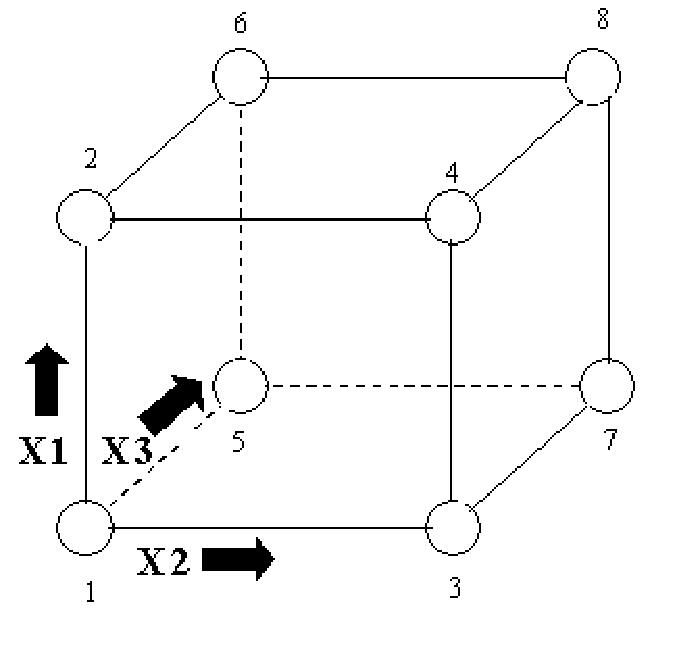
\includegraphics[scale=0.6]{cube}
  \end{center}
  \caption[Laatikkokuvaaja]{Täysyhdistelykokeen graafinen esitys, ns. "laatikkokuvaaja".}
  % Optional shorter caption in brackets is used in Table of Figures
  % (tof).
  \label{fig:cube}
\end{figure}






Käytetyin koesuunnitelma on \textit{osittainen yhdistelykoe} (engl. fractional factorial
design), useimmiten 2 tai 3:lla tekijätasolla. Osittaisessa kokeessa ei ajeta
kaikkia mahdollisia yhdistelmiä, vaan vain tietyt tarkoituksella valitut. Hyvä
osittainen yhdistelykoe antaa tyydyttävästi tietoa yhteisvaikutuksista
kohtuullisella koemäärällä.

Osittaisista yhdistelykokeista käytetään merkintää \(I^{k - p}\)
mikä tarkoittaa että koe on \(1/I^p\)-osa \(I^k\)-kokeesta.
Esimerkiksi \(2^{3 - 1}\)-koe on puolikas \(2^3\)-kokeesta,
jolloin koeajoja on vain 4 (\(2^3\)-kokeessa koeajoja on 8).
\(2^{6-2}\)-koe on neljäsosa \(2^6\)-kokeesta
ja siinä on 16 koeajoa.

Pienempi koemäärä johtaa tekijöiden vaikutusten
\textit{sulautumiseen}
(engl. \textit{aliasing} tai \textit{confounding}), mikä tarkoittaa että joitain
vaikutuksia ei voida erottaa toisistaan. Esimerkiksi tekijä A ja yhteisvaikutus BCD
voivat olla sulautuneita, jolloin ei voida sanoa johtuuko vaikutus A:sta vai
BCD:stä. Mitä vähemmän koeajoja on, eli mitä osittaisempi suunnitelma on, sitä
enemmän on sulautumisia. Suunnitelmien teossa käytetään hyväksi n.s.
\textit{vaikutusten niukkuusperiaatetta} (engl. \textit{sparsity-of-effects principle}),
jonka mukaan todennäköisintä on että vaikutuksen aiheuttaa yksi tekijä, vähemmän
todennäköistä on kahden tekijän yhteisvaikutus, vielä vähemmän todennäköistä on
kolmen tekijän yhteisvaikutus jne.
Suunnitelmissa monen tekijän yhteisvaikutukset
yleensä sulautetaan ja kokeen tekijän on hyvä ottaa tämä huomioon.
Yhden tekijän aiheuttamia vaikutuksia vasteeseen kutsutaan \textit{päävaikutuksiksi}
(engl. \textit{main factor}) erotukseksi useamman tekijän yhteisvaikuksista.

Nykyisin tietokoneiden avulla voidaan luoda algoritmin tuottamia D-optimaalisia
koesuunnitelmia. Suunnitelman luova algoritmi etsii optimaalisen ryhmän
koeajoja mahdollisten koeajojen joukosta siten että mallin parametriarvioiden
kovarianssi miminoituu \parencite[s.~513]{Montgomery2012}.
Toisin kuin yleiset koesuunnitelmat, D-optimaaliset eivät välttämättä ole
ortogonaalisia ja siten vaikutusarviot voivat olla toisistaan riippuvaisia.
Ne kuitenkin sallivat kokeen suorittamisen tavallisia koesuunnitelmia
vähemmillä koeajoilla ja sallivat suunnitelman muokkauksen silloin kun
kaikkia tekijätasojen yhdistelmiä ei syystä tai toisesta voida toteuttaa
\parencite{ehandbook}.
D-optimaalinen suunnitelma kykenee arvioimaan kaikki yhden parametrin vaikutukset sekä kaikki 2 tekijän yhteisvaikutukset pitämällä koeajojen määrän kuitenkin mahdollisimman pienenä.



\textcite{Li2006} ovat tehneet meta-analyysin yhdistelykokeissa esiintyvistä
säännönmukaisuuksista, joista yksi on em. vaikutusten niukkuusperiaate.
Analyysin tuloksia on muun muassa:

\begin{itemize}
\item Kaikki yleensä kirjallisuudessa käsitellyt säännönmukaisuudet, joista yhtenä
    vaikutusten niukkuusperiaate, vahvistettiin tilastollisesti merkittäviksi mutta
    heikommiksi kuin mitä niiden käsittely usein antaa ymmärtää.
\item Riippuen tekijöiden määrästä, kolmen tekijän yhteisvaikutuksia voi esiintyä
    enemmän kuin kahden tekijän yhteisvaikutuksia.
\end{itemize}

Tuloksia voidaan mallintaa matemaattisesti, vasteen ja tekijöiden yhdistävällä
yhtälöllä. Ensimmäisen kertaluvun malli kuvaa ainoastaan tekijöiden päävaikutuksia.
Jos tekijöitä on esimerkiksi kaksi, on malli

\begin{equation}
  \label{eq:1krtluku}
 y = \beta _0 + \beta _{1}x_1 + \beta _{2}x_2 + \varepsilon,
\end{equation}

missä \textit{y} on vaste, \textit{x}:t tekijöitä, $\beta $:t tuntemattomia parametreja
jotka arvioidaan kokeen tuloksista ja $\varepsilon $ on
kokeessa tapahtuvaa satunnaista virhettä kuvaava termi.
Usein lisätään yhteisvaikutusta kuvaava termi, esimerkiksi kahden tekijän tapauksessa

\begin{equation}
  \label{eq:2krtluku}
 y = \beta _0 + \beta _{1}x_1 + \beta _{2}x_2 + \beta _{12}x_{1}x_{2} + \varepsilon,
\end{equation}

jolloin voidaan kuvata päävaikutuksia ja kahden tekijän yhteisvaikutuksia.



Koesuunnitelmaan ja sulauttamiseen liittyy käsite \textit{resoluutio}. Resoluutio
kertoo kuinka monet vaikutukset suunnitelmassa on sulautettu. Arvo ilmoitetaan
roomalaisilla numeroilla ja isompi resoluutio tarkoittaa vähemmän sulautumisia.
Yleensä on siis järkevää valita suurin mahdollinen resoluutio ottaen huomioon
koeajojen määrä. Yleisimmät resoluutioarvot ovat III, IV ja V:

\begin{description}
\item[Resoluutio III] Päävaikutukset eivät ole sulautuneita toisiinsa
mutta ovat sulautuneita 2 tekijän yhteisvaikutuksiin;
\item[Resoluutio IV] Päävaikutukset eivät ole sulautuneita toisiinsa eivätkä 2 tekijän
yhteisvaikutuksiin mutta jotkut 2 tekijän yhteisvaikutukset ovat sulautuneita toisiinsa
ja päävaikutukset ovat sulautuneita 3 tekijän yhteisvaikutuksiin;
\item[Resoluutio V] Päävaikutukset ja 2 tekijän yhteisvaikutukset eivät ole sulautuneita
keskenään tai toisiina mutta 2 tekijän yhteisvaikutukset ovat sulautuneita 3 tekijän
yhteisvaikutuksiin ja päävaikutukset ovat sulautuneita 4 tekijän yhteisvaikutuksiin. \parencite[s.~9]{montgomery2006}
\end{description}




Yksinkertaisin tapa toteuttaa koe on vaihdella yhtä tekijää kerrallaan
muiden pysyessä valituilla perustasoillaan ja toistaa
tämä kaikille tekijöille vuorollaan. Tätä kutsutaan
yksi tekijä kerrallaan -menetelmäksi
(engl. one-factor-at-a-time tai OFAT).
Tuloksista on helppo piirtää yksinkertaisia vaikutuskuvaajia
\todo{vaikutuskuvaajat}.
OFAT ei kuitenkaan pysty havaitsemaan
tekijöiden yhteisvaikutuksia,
vaatii enemmän koeajoja
ja voi helposti olla huomaamatta tekijöiden optimiyhdistelmiä.
Siten esimerkiksi \textcite{Montgomery2012}
yhtyy siihen yleiseen käsitykseen että käytännössä joka tilanteessa on
suotavampaa käyttää yhdistelykokeita koska yhteisvaikutukset
ovat niin yleisiä ja silloin OFAT ei toimi hyvin.
Kuitenkin \textcite{frey2005mechanisms} osoittavat tämän
olevan ainakin osittain virheellinen käsitys. Heidän tutkimansa
menetelmä on adaptive OFAT (aOFAT, mukautuva OFAT), jossa muutetaan
yhtä tekijää, tarkistetaan tulos, ja jos se on parempi niin
pidetään tekijä tällä tasolla ja jos huonompi niin muutetaan se
takaisin aiemmalle. Näin jatketaan kunnes kaikkia tekijöitä on
muutettu. Tutkimuksen mukaan ainakin tämä menetelmä voi
johtaa keskimäärin parempiin tuloksiin jos kokeen virhe on
pieni (vähemmän kuin yksi neljäsosa tekijävaikutuksista) tai
tekijöitten yhteisvaikutukset suuria (enemmän kuin yksi neljäsosa
kaikista vaikutuksista). \textcite{frey2005mechanisms} esittävät
myös mekanismeja ja selityksiä tälle tulokselle.


Kokeen suunnittelun alkuvaiheessa monia mahdollisia tekijöitä harkitaan
mutta todennäköisesti useat niistä ovat merkityksettömiä tai lähes
merkityksettömiä. Tätä ei kuitenkaan voida etukäteen tietää. Tällöin
on tarkoituksenmukaista tehdä \em seulontakoe, \em
(engl. \em screening experiment\em) jossa mukana on monia tekijöitä
ja tarkoituksena on tunnistaa niistä ne joilla on suuri vaikutus.
Tärkeiksi havaitut tekijät tutkitaan perusteellisemmin myöhemmissä
kokeissa.

Hyödyllisintä seulontakokeessa on käyttää osittaista
yhdistelykoetta, jossa koeajojen määrä pysyy kohtuullisena
useasta tutkittavasta tekijästä huolimatta.
Usein hyödyllisin suunnitelma on kaksitasoinen \(2^{k - p}\)-koe.
Yleensä seulontakokeeksi valitaan
resoluution III tai IV koe \parencite[s.~9]{montgomery2006}.
On kuitenkin pidettävä mielessä näiden resoluutiotasojen
toimivuuden perustuvan vaikutusten niukkuusperiaatteelle.

\textcite{plackett1946} esittivät Plackett-Burman-suunnitelmat,
jotka ovat erittäin vähän koeajoja sisältäviä osittaisia yhdistelykokeita
ja soveltuvat siten hyvin käytettäväksi seulontaan. Esimerkiksi 12 koeajon
PB-suunnitelmassa voidaan tutkia 11 tekijää. Näissä suunnitelmissa
päävaikutukset ovat kuitenkin voimakkaasti sulautuneet yhteisvaikutuksiin.



Seulontakokeen perusteella jatkokokeita voidaan säätää monella tavalla.
Tekijöitä voidaan poistaa tai lisätä, niiden vaihteluvälejä voidaan
säätää sopivammiksi, joitakin seulontakokeen koeajoja voidaan toistaa
virheen tai jonkin muun syyn vuoksi ja koealuetta voidaan säätää
seulonnassa havaitun suuntauksen mukaan.
\textcite{box1993} ovat esittäneet Bayesilaisen menetelmän
aktiivisten tekijöiden tunnistamiseen seulontakokeessa.



Koeajojen jälkeen tulokset analysoidaan tilastollisilla menetelmillä.
Koesuunnitteluun tarkoitetut ohjelmistot tekevät tämän yleensä
automaattisesti, mutta osaavat kokeentekijät voivat myös tehdä
analyyseja itse esimerkiksi python tai R -ohjelmointikielillä.
Usein hyödyllisintä datan tutkimiseen ja tulkintaan on
piirtää yksinkertaisia kuvia ja kuvaajia.



\section{Dispersiovaikutukset, robusti suunnittelu ja optimointi}

Teollisuudessa prosessin tuloksena on usein jokin tuote, ja vasteena voidaan
tutkia jotakin tämän tuotteen ominaisuutta. Koesuunnittelun menetelmillä
saadaan selville tutkittavien tekijöiden vaikutus tähän ominaisuuteen.
Yleensä tuotteen ominaisuuksien halutaan pysyvän aina samana kun
tekijät pidetään tietyillä tasoilla. Tällöin tuote on tasalaatuista, mikä
on yksi laadunhallinnan tavoitteista.

Vasteen satunnaista vaihtelua sanotaan \em varianssiksi \em tai \em vaihteluksi, \em
ja yleensä tavoitellaan sen minimoimista. Koesuunnittelulla saadaan
tietoa tekijöiden vaikutuksista vasteen varianssiin. Tällaista vaikutusta
kutsutaan \em dispersiovaikutukseksi. \em
Vastaavasti kuten edellä käsitellyissä vaikutuksissa vasteen tasoon,
myös dispersiovaikutuksissa esiintyy yhden tekijän päävaikutuksia
ja monen tekijän yhteisvaikutuksia.


Kun koesuunnittelulla halutaan saada selville nämä vaikutukset
ja se ihanteellinen tekijätasojen yhdistelmä jolla varianssi on pienimmillään,
puhutaan \em robustien parametrien suunnittelusta \em (engl. \em robust
parameter design\em, robustien koska prosessista halutaan mahdollisimman
vastustuskykyinen satunnaisille muutoksille, so. robusti, ja parametrien koska
teollisuudessa kokeen tekijät ovat yleensä hallittavia prosessiparametreja).
Dispersiovaikutusten etsintään on kolme lähestymistapaa:

\begin{enumerate}
\item  Kokeessa toistetaan koetta samalla hallittavien tekijöiden
    tasolla josta varianssia voidaan arvioida;
\item Kokeeseen pakotetaan varianssia sisällyttämällä siihen
    myös ei-hallittavia tekijöitä;
\item Dispersiovaikutuksia analysoidaan kokeista joissa ei
    ole toistoa. \parencite{Bursztyn}
\end{enumerate}

Ensimmäistä ja kolmatta lähestymistapaa kutsutaan joskus
\em passiiviseksi \em robustiksi suunnitteluksi ja toista lähestymistapaa
\em aktiiviseksi \em robustiksi suunnitteluksi.

Ei-hallittavien tekijöiden sisällyttäminen oli japanilaisen
Genichi Taguchin (1924 - 2012) idea. Taguchi kehitti menetelmänsä
1950-luvulla ja ne saivat suurta huomiota Yhdysvalloissa 1980-luvulla.
Taguchi vaikutti siten voimakkaasti laadunhallinnan tekniikan kehittymiseen.

\subsection{Taguchi-menetelmä}

Taguchi esitti että vasteen vaihtelun aiheuttavat usein satunnaiset vaihtelut
merkittävissä tekijöissä joita ei kuitenkaan voida prosessin aikana hallita.
Esimerkkejä ovat ympäristötekijät, kuten ilmankosteus tai lämpötila, ja
komponenttien mittojen vaihtelu nimellisarvon ympärillä (toleranssit).
Taguchi nimesi nämä ei-hallittaviksi tekijöiksi (noise factor)
ja erotti ne hallittavista tekijöistä antaen niille kokeessa erityistä
huomiota. Tavoitteeksi hän asetti niiden hallittavien tekijöiden tasojen
löytämisen, joilla ei-hallittavien tekijöiden dispersiovaikutus minimoituu.
\textcite{Bursztyn} antavat yksinkertaisen esimerkin ei-hallittavien tekijöiden
sisällyttämisestä: Ajatellaan että koe tehdään tuotteelle jonka
komponenttiosan leveys on \(3,0 \pm 0,1\) mm.
Toistoon perustuvassa dispersiovaikutusten etsinnässä jokainen
komponenttiosa valittaisiin satunnaisesti, joten joittenkin leveys
saattaisi olla 2,9 mm, joittenkin 3,1 mm, mutta monet olisivat lähellä
3,0 mm. Taguchin menetelmässä komponentin leveys valittaisiin
ei-hallittavaksi tekijäksi ja kokeessa käytettäisiin vain niitä joiden
leveys on 2,9 mm tai 3,1 mm. Koesuunnitelmaan sisältyisi tällöin
kaksitasoinen ei-hallittava tekijä jonka matala taso on 2,9 mm ja
korkea taso 3,1 mm.

Hyvä esimerkki on japanilaisen Ina Tile Companyn tapaus 1950-luvulta,
kuten \textcite{Kackar1989} kertoo:
Yhtiön valmistamien tiilien mitat vaihtelivat paljon ja monet olivat sallittujen mittojen ulkopuolella
jolloin hävikki oli suurta.
Saatiin selville että vaihtelua aiheutti polttouunin epätasainen lämpötila,
jota ei kuitenkaan voitu hallita. Taguchi-menetelmillä saatiin selville että
lisäämällä kalkin määrää savessa, mikä taas oli hallittava tekijä, tiilet saatiin
vastustuskykyisemmiksi uunin lämpötilan vaihtelulle ja mitat yhdenmukaisemmiksi.

\todo{regression slope kuvaaja}.
\textcite{steinberg1994,Steinberg1998,Berube1998} ovat osoittaneet
että ei-hallittavien tekijöiden sisällyttäminen kokeeseen voi
lisätä sen kykyä havaita dispersiovaikutuksia huomattavasti.
Haittapuolia ovat kuitenkin koeajojen määrän huomattava lisääntyminen
ja se, että tämänkaltaisia tekijöitä on usein vaikea
tai kallista hallita kokeen aikana. Luonnollisesti jotta merkittävät ei-hallittavat
tekijät voidaan sisällyttää kokeeseen, on ne tunnistettava oikein jo
suunnitteluvaiheessa, mikä vaatii usein erinomaista prosessin tuntemusta
eikä suinkaan ole itsestäänselvää.

Taguchin menetelmässä hallittaville ja ei-hallittaville
tekijöille valitaan omat erilliset koesuunnitelmansa.
Hallittavien tekijöiden suunnitelmaa nimitetään \em sisätaulukoksi \em
ja ei-hallittavien tekijöiden suunnitelmaa \em ulkotaulukoksi \em
(engl. \em inner array\em ja \em outer array\em).
Nämä suunnitelmat
"ristitään", so. sisätaulukon jokainen tekijätasojen yhdistelmä
suoritetaan ulkotaulukon joka tekijätasojen yhdistelmällä. Syntyvää
koesuunnitelmaa sanotaan \em ristikkäiseksi suunnitelmaksi \em
(engl. crossed array design). Kuvassa \ref{subfig:crossed} on esimerkki tällaisesta suunnitelmasta.
Kuvan sisätaulukko on \(2^{4-1}\) osittainen yhdistelykoe ja ulkotaulukko
yksinkertainen \(2^1\)-koe. Sisätaulukon 8 koeajoa ja ulkotaulukon 2
ristiöitynä tekevät yhteensä 16 koeajoa, mutta kuvan kokeessa jokainen
yhdistelmä myös toistettiin kolmesti, tuloksena 48 havaintoa.
Kuvassa \ref{subfig:crossed2}
on toinen esimerkki ristikkäisestä suunnitelmasta. Nyt sisätaulukossa
on kolmitasoinen resoluution III \(3^{4-2}\)-suunnitelma ja ulkotaulukossa \(2^3\)-suunnitelma,
yhteensä \(9\times 8=72\) koeajoa. Kuten nähdään, vaikka tekijöitä on vain
7 ja resoluutio vain III, on koe silti suhteellisen aikaavievä.


\begin{figure*}
  \begin{center}
    \subfigure[Ristikkäinen Taguchi-suunnitelma kolmella koetoistolla \parencite{Montgomery2012}.]{
      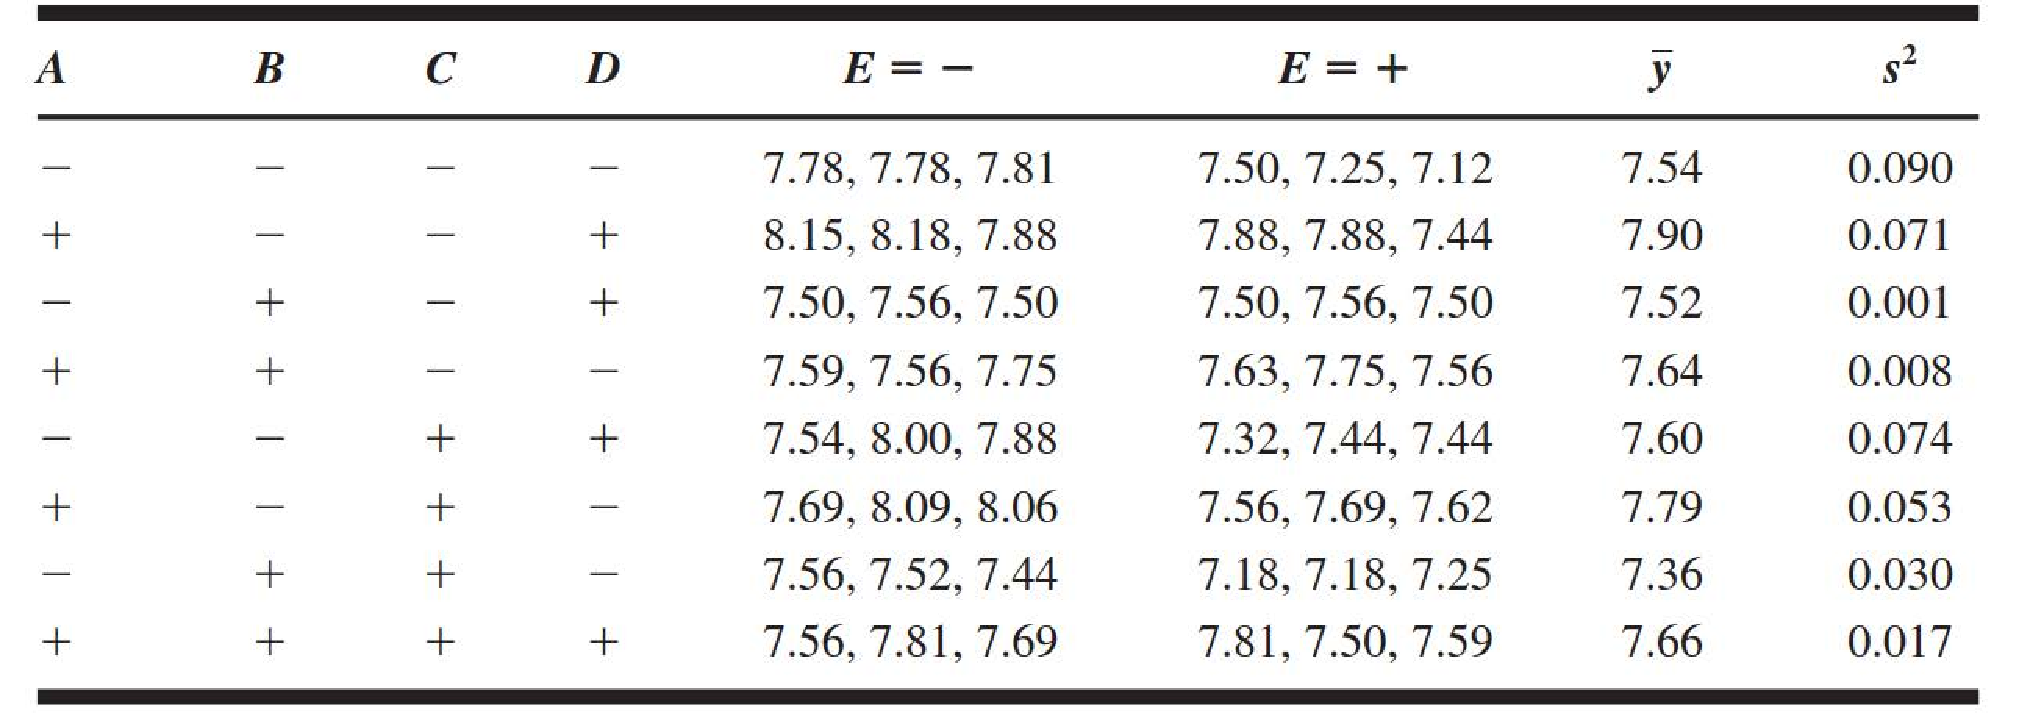
\includegraphics[width=\textwidth]{crossed}
      \label{subfig:crossed}}
    %\qquad                        % i) Ugly hack to get more horizontal space between figures
    %\hspace{0.05\textwidth}      % ii) Another ugly way to hack space
    % ~~                          % iii) Yet another...

    \subfigure[Ristikkäinen Taguchi-suunnitelma \parencite{byrne1987taguchi}.]{
      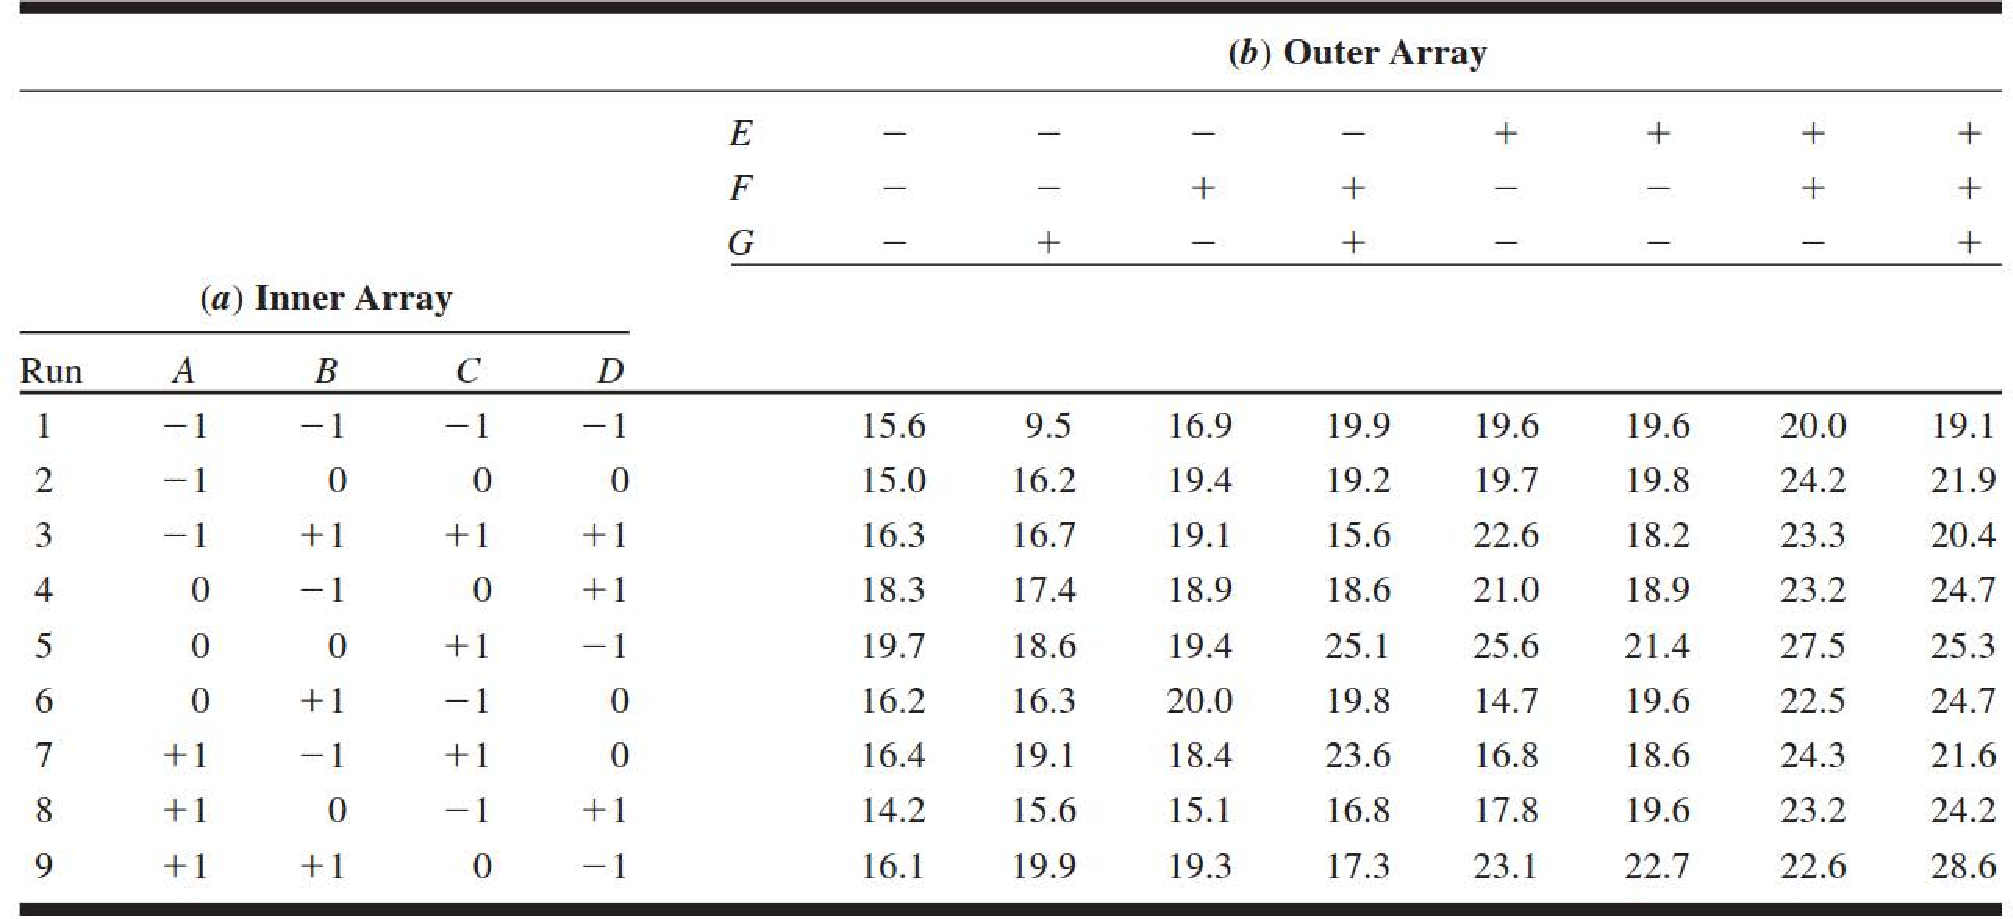
\includegraphics[width=\textwidth]{crossed2}
      \label{subfig:crossed2}}
    \caption[Ristikkäisiä suunnitelmia]{Ristikkäisiä Taguchi-suunnitelmia.}
    % Optional shorter caption in brackets is used in Table of Figures
    % (tof).

    \label{fig:prosessi}
  \end{center}
\end{figure*}




\textcite{shoemaker1991} huomauttavat että tällainen ristikkäinen
suunnitelma on pohjimmiltaan vain osittainen yhdistelykoe jolla
on tietty sulautumisrakenne. Kun ristikkäinen suunnitelma esitetään
näin, puhutaan \em yhdistetystä suunnitelmasta \em (eng. \em combined
array\em). Yhdistetyssä suunnitelmassa ei-hallittavia
tekijöitä ei siis eroteta omaksi ulkotaulukokseen, vaan niitä vaihdellaan yhdessä hallittavien
tekijöiden kanssa kuten normaalissa \(2^k\)-kokeessa.
Yhdistetyn suunnitelman etuna on suurempi joustavuus, sillä siinä sulautumisia
voidaan hallita tarpeen mukaan.
\textcite{Hijar-Rivera2009} esittävät tietokoneella tuotettuja ristikkäisiä
suunnitelmia Taguchin tarjoamien valmiiden suunnitelmien rinnalle.
Jokaiselle Taguchin suunnitelmalle voitiin tuottaa vähintään yksi koeajoiltaan samansuuruinen
mutta tehokkaampi suunnitelma.

Myös Taguchin menetelmä ristikkäisen suunnitelman datan analysointiin on
omintakeinen. Ei-hallittavia tekijöitä sisältävien kokeiden analysoinnissa
käytetään pääasiassa kahta menetelmää, vastemallianalyysia ja suoritemitta-analyysia
(engl. response model analysis ja performance measure analysis).
Suoritemitta-analyysi on Taguchin kehittämä menetelmä, jossa
tulokset joka hallittavien tekijätasojen yhdistelmästä yhdistetään matemaattisesti
"suoritemitaksi", jonka riippuvuutta hallittavista tekijöistä vuorostaan
analysoidaan. Käytetyin Taguchin kehittämistä suoritemitoista on
\em signaali-kohinasuhde, \em joka kuvaa vasteen keskiarvon suuruutta suhteessa
sen varianssiin. Hallittavien tekijöiden dispersiovaikutukset tunnistetaan
niiden vaikutuksesta signaali-kohinasuhteeseen, ja robustin suunnittelun
tavoitteena on maksimoida tämä suhde.
Suoritemitta-analyysin tarkoituksenmukaisuutta on kritisoitu paljon.
\textcite{Bursztyn} mukaan sen suurin heikkous on siinä että
kokeeseen sisällytettyjä ei-hallittavia tekijöitä ei
erityisesti hyödynnetä,
vaikka ne on varta vasten tunnistettu ja valittu koetta varten. Pohjimmiltaan
niiden data vain "luhistetaan" matemaattisesti jonka jälkeen analyysi
tehdään kuten yksinkertaisessa toistoon perustuvassa suunnitelmassa.
Toinen ongelmallinen seikka on vasteen keskiarvon ja sen varianssin
väkinäinen yhdistäminen.
\textcite{box1988,steinberg1994} ovat näyttäneet monia muitakin suoritemitta-analyysin
haittoja, mm. sen että se voi olla huomaamatta dispersiovaikutuksia.

Vastemallianalyysi on vähemmän kiistanalainen analysointimenetelmä.
Sovellettuna yhdistettyyn suunnitelmaan se on samankaltainen kuin
luvussa \ref{doe} esitetty tulosten mallintamisen
menetelmä. Esimerkiksi, jos on 2 hallittavaa tekijää, $x_1$ ja $x_2$, ja yksi
ei-hallittava tekijä, $z_1$, malli on

\begin{equation}
  \label{eq:vastemalli}
 y = \beta _0 + \beta _{1}x_1 + \beta _{2}x_2 + \beta _{12}x_{1}x_{2} + \gamma _{1}z_1 + \delta _{11}x_{1}z_{1} + \delta _{21}x_{2}z_1 + \varepsilon
\end{equation}

Keskiarvo ja varianssi voidaan mallintaa myös ristikkäisestä suunnitelmasta suoraan.
Arvot lasketaan joka sisätaulukon koeajoyhdistelmälle
samojen ei-hallittavien tekijöiden arvojen tasolla,
joten niissä esiintyvät erot johtuvat hallittavien tekijöiden eri tasoista. Voidaan
siis yhtä aikaa optimoida sekä vasteen keskiarvo että sen varianssi.




Taguchin menetelmien perusteista ja pätevyydestä on huomattavasti erimielisyyttä.
Yleisesti ottaen tilastotieteilijät, matemaatikot ja tutkijat sanovat menetelmän
olevan vanhentunut ja kritisoivat joustamattomuutta (koe pitää muokata
annettujen suunnitelmien mukaiseksi, kun taas tietokoneiden avulla suunnitelmat
voidaan luoda kokeen perusteella,
kokeen tekijän on tunnettava prosessi erittäin hyvin
jotta mahdollisia merkittäviä mutta ennalta tuntemattomia tekijöitä
ei jää huomiotta), tehottomuutta (pieni resoluutio suhteessa
koeajojen määrään) ja annettujen analysointityökalujen järkevyyttä
(signaali-kohinasuhde).
Yksi ongelma on myös se että hieman ulkopuolisena uudistajana Taguchi
usein turhaan uudelleennimesi jo olemassa olevia käsitteitä ja käytti
erikoisia merkintöjä, jotka ovat yhä käytössä näissä menetelmissä.
Esimerkiksi hallittavien ja ei-hallittavien tekijöiden nimeäminen
control- ja noise factoreiksi kun tilastotieteessä noise-sanalla (kohina)
on jo oma merkityksensä aiheuttaa tarpeetonta sekaannusta.
Sama pätee robust-sanaan.
Toisaalta Taguchi-menetelmiä
on teollisuudessa käytetty jo kauan (kuten esimerkiksi Six Sigma -strategiassa)
ja tulosten ja käyttäjien kokemusten perusteella se on usein
toiminut paremmin kuin tarjotut vaihtoehdot.
\textcite{Berube1998} huomauttavat että osa ongelmaa on se että
monet käytetyistä tulosten analysointimenetelmistä eivät ole
erityisesti käyttäneet hyväksi ristikkäisen suunnitelman ja ulkotaulukon
rakennetta.
\textcite[s.~554]{Montgomery2012} mukaan vastepintamenetelmä
(josta lisää luvussa \ref{vastep})
on luotettavampi ja tehokkaampi vaihtoehto robustien parametrien suunnitteluun.
\textcite{Sleeper2012} jättää Taguchi-menetelmät kokonaan
pois kirjastaan sanoen niiden käytön olevan vähentymässä ja tarjoaa myös tilalle
vastepintamenetelmää.

\textcite{Antony2006} antaa yleistason kuvan Taguchi-menetelmien ja
perinteisen koesuunnittelun eroista harjoittajan näkökulmasta. Taulukossa \ref{tab:vertailu}
hän vertailee Taguchi-menetelmää ja perinteistä koesuunnittelua, jolla hän
tässä tarkoittaa seulontakoe-vastepinta-menetelmää josta lisää luvussa \ref{vastep}.
Antony näyttää kallistuvan Taguchi-menetelmän kannalle teollisuuden
tarpeiden tapauksessa.

\begin{table}
  \small
  \begin{center}
    \caption{Robustien parametrien suunnittelumenetelmän valinnan kaavio \parencite{Antony2006}.}
    \label{tab:vertailu}
    \begin{tabular}{l | c c c c c c}
      % l = align to left (e.g. text), c=align to center, r=align to
      % right (e.g. numbers), Pipe | creates vertical line
      % Let's put 1 horinzontal line above the table, 2 after header rows,  and 1 below
      \hline
      \textbf{Ongelman luonne} & \textbf{Taguchi}& \textbf{Perinteinen}  \\
                         & \textbf{DOE}     & \textbf{DOE} \\
      \hline 
      \hline
      Kokeen tekijä uskoo tutkimuskohteessa olevan läsnä vahvoja vuorovaikutuksia & \times & \checkmark \\
      
      Nopea prosessin yleistuntemus ja vastaus johtoportaalle & \checkmark & \times   \\
      
      Prosessin optimiolosuhteiden määritys & \times & \checkmark \\
      
      Robusti suunnittelu kun ei-hallittavat tekijät on tunnistettu vaihtelun lähteiksi & \checkmark & \times \\
      
      Prosessin suorityskykymitan tavoitearvon ennakointi & \times & \checkmark \\
      
      Varianssin vähentäminen tietyn tavoitearvon läheisyydessä & \checkmark & \times \\
      
      Vasteen ja prosessiparametrien välisen suhteen matemaattinen mallintaminen & \times & \checkmark \\
      
      Parametrien ja toleranssien suunnittelu halutun varianssin saavuttamiseksi & \checkmark & \times \\
      \hline
    \end{tabular}
  \end{center}
\end{table}



\textcite[s.~300-301]{Hedayat2012} luettelevat
seuraavat ongelmat liittyen
Taguchi-menetelmiin:
\begin{itemize}
\item Signaali-kohinasuhde ei kerro kuinka hallittavat tekijät vaikuttavat
      vasteeseen. Vaikka vaikutusta havaittaisiin, ei silti voida tietää
      muuttaako se vasteen tasoa, varianssia vai molempia.
\item Mahdollisia tekijöitten välisiä vuorovaikutuksia (huom. ei siis yhteisvaikutuksia) ei oteta huomioon.
\item Vaikka ristikkäisyyden vuoksi koeajoja ja tuloksia on paljon, hallittavien tekijöiden
    tasoyhdistelmiä on kuitenkin suhteessa tähän vain pieni määrä. Siten hallittavien
    tekijöiden keskinäinen sulautuminen on aina sama, ja täten ko. resoluutio pieni.
\item Menetelmä ei kerro tarkalleen kuinka ei-hallittavat tekijät vaikuttavat vasteeseen.
      Syntyykö kohina vain joistain ei-hallittavista tekijöistä? Onko niitten ja
      hallittavien tekijöitten välillä vuorovaikutuksia? Signaali-kohinasuhdeanalyysi
      ei vastaa näihin kysymyksiin.
\end{itemize}

\textcite{nair1992} ovat koonneet kattavan paneelikeskustelun Taguchi-menetelmän
toimivuudesta. Yksi väittelyn ydinkohdista on ristikkäisten ja yhdistettyjen suunnitelmien
tehokkuudesta robustissa suunnittelussa.
Teoreettiset perustelut yhdistettyjen suunnitelmien toimivuudelle ovat
vakuuttavat mutta jotkut empiiriset kokeet viittaavaat siihen että
ristikkäiset suunnitelmat johtavat parempiin tuloksiin
\parencite{kunert2003experiment}.
\textcite[s.~558]{Montgomery2012} on sitä mieltä että yleensä ottaen yhdistetyt
suunnitelmat ovat paljon tehokkaampia.
Osa erimielisyyksistä liittyy siihen, missä määrin ns. vaikutusten
niukkuusperiaatetta pidetään perusteltuna \parencite{Li2006}.

\textcite{Bursztyn} vertailevat kattavassa tutkimuksessaan menetelmiä dispersiovaikutusten
seulomiseksi. He päätyvät siihen tulokseen että ei-hallittavien tekijöiden
sisällyttäminen kokeeseen lisää huomattavasti kokeen kykyä havaita
dispersiovaikutuksia verrattuna pelkästään kokeiden toistoon perustuvaan
kokeeseen. He huomasivat että tämä parannus saavutetaan vain
kun
tulosten analysointiin
käytetään vastemallianalyysia, \em ei silloin kun käytetään Taguchin kehittämää
suoritemitta-analyysia. \em
Lisäksi \textcite{Bursztyn} päätyivät siihen tulokseen että dispersiovaikutusten
havaitseminen kokeista joissa ei ole toistoa on hyvin riskialtista eikä
sen yrittäminen suotavaa.

\subsection{Vastepintamenetelmä}
\label{vastep}

Vastepintamenetelmä (engl. response surface methodology, RSM)
on kokoelma matemaattisia tekniikoita jotka soveltuvat erityisen hyvin tilanteisiin
joissa vaikuttaa monia tekijöitä ja tavoitteena on vasteen optimointi, kuten
robustien parametrien suunnittelussa. Nimi tulee menetelmässä piirrettävistä
kuvaajista joissa vaste usein esitetään kaksiulotteisena pintana kuten \todo{kuvassa n}.
Vastepintamenetelmän loppuvaiheen optimointiin kehitetyt koesuunnitelmat
keskittyvät tekijöiden ja vasteen välisen suhteen mallintamiseen
eivätkä ne sovellu merkittävien tekijöiden tunnistamiseen eli seulontaan kuten $2^k$-suunnitelmat
soveltuvat. Usein näitä suunnitelmia käytetäänkin peräkkäin jolloin 
$2^k$-seulontakokeessa tunnistettuja tekijöitä optimoidaan tarkemmilla vastepintasuunnitelmilla.
\textcite{ehandbook} mukaan vastepintasuunnitelmiin on paras siirtyä vasta
sitten kun seulontakokeella on vähennetty tutkittavien tekijöiden määrää
neljään tai vähempään.

Usein tekijöiden seulonnan jälkeen prosessin senhetkisten tekijätasojen oletetaan
vielä olevan kaukana optimista, joten on suotavaa ensin siirtyä nopeasti optimialueen
läheisyyteen, jonka jälkeen vasta mallinnetaan vastepinta ja tarkemmat tekijöiden
optimitasot. Ensimmäinen tai ensimmäiset kokeet voidaan tehdä $2^k$-suunnitelmilla
ja  sovittamalla tulokset ensimmäisen kertaluvun malliin \ref{eq:1krtluku}.
Tämän jälkeen kohti optimialuetta siirrytään \em jyrkimmän nousun \em
(tai \em jyrkimmän laskun \em) menetelmällä. Jyrkimmän nousun suunta on se
suunta, missä vaste $y$ nousee nopeimmin. Ensimmäisen kertaluvun mallissa,
jossa ei ole kaarevuutta, tämä suunta on kohtisuora vastepintaa kohden, kuten
nähdään kuvasta \todo{kuva jossa steepest ascent}. Kokeen tekijä päättää
kuinka isoja askeleita jyrkimmän nousun suuntaan otetaan. Uusia kokeita suoritetaan
aina askelten välissä, ja jos vasteessa ei enää havaita nousua, voidaan sovittaa
uusi ensimmäisen kertaluvun malli, jonka jälkeen jatketaan samaan tapaan.
Lopulta päädytään lähelle optimialuetta, mistä yleensä kertoo ensimmäisen kertaluvun mallin
huonompi sopivuus tuloksiin.

Optimialueen läheisyydessä toteutetaan vastepintasuunnitelma, josta voidaan
tarkasti arvioida vastepinnan muotoa ja siten myös tekijöiden optimitasoja.
Yleisimmin käytetyt suunnitelmat ovat Box-Behnken- ja keskiökomposiittisuunnitelmat
(engl. Central composite design, CCD). Molemmissa käytetään vähintään kolmea
tekijätasoa kaarevuudeen mallintamiseksi. Joissain CCD-suunnitelmissa vaaditaan
jopa viisi tekijätasoa. Taulukossa \ref{vpsuunnitelmat} nähdään näitten suunnitelmien vaatimat
koeajojen määrät eri tekijöiden määrällä.

\begin{table}[]
\centering
\caption{CCD- ja Box-Behnken-suunnitelmien vaatimat koeajojen määrät eri tekijöiden määrällä \parencite{ehandbook}}
\label{vpsuunnitelmat}
\begin{tabular}{ccc}
\hline
\textbf{Tekijöiden määrä} & \textbf{CCD-suunnitelma}                 & \textbf{Box-Behnken} \\ \hline
2                         & 13                                       & -                    \\
3                         & 20                                       & 15                   \\
4                         & 30                                       & 27                   \\
5                         & 33 (osittainen) tai 52 (täydellinen koe) & 46                   \\
6                         & 54 (osittainen) tai 91 (täydellinen koe) & 54                  
\end{tabular}
\end{table}

Jotta vastepintamenetelmällä saadaan mallinnettua vasteen varianssia, on käytettävä
passiivista robustien parametrien suunnittelua, eli
joka koeajosta on tehtävä useita toistoja. Toistoista lasketaan joka pisteelle vasteen
varianssi, joka pyritään tässä tapauksessa minimoimaan. Toistojen vuoksi
kokeiden määrä saattaa nousta kokeesta riippuen hyvin korkeaksi.


\subsection{Muut menetelmät}

\textcite{frey2008adaptive} ovat tutkineet adaptive OFAT (mukautuva OFAT) -menetelmän
toimivuutta robustissa suunnittelussa. Menetelmä on kuten kappaleessa \ref{doe} mainittu
aOFAT, erotuksena se että joka hallittavan tekijän tason vaihdon
jälkeen ajetaan ei-hallittaville tekijöille resoluutio III -tasoinen
yhdistelykoe. Johtopäätöksenä he esittävät että OFAT on tässäkin tilanteessa
turhaan ylenkatsottu menetelmä.

Kun kokeen virhe on pieni
tai yhteisvaikutukset suuria, on
tämänkaltainen aOFAT parempi kuin Taguchi-tyyliset ristikkäiset suunnitelmat.
Kun virhe kasvaa, tietyssä pisteessä ristikkäiset suunnitelmat osoittatuvat
kuitenkin paremmiksi.


Minitab ja useimmat muut koesuunnitteluohjelmistot tarjoavat työkalut
Taguchi- ja vastepintasuunnitelmien tekoon ja tulosten analysointiin.
Aina ne eivät kuitenkaan tarjoa dispersiovaikutusten ja vasteen varianssin
analysointiin tarvittavia valmiita suunnitelmia, ja kokeentekijän
on itse suunniteltava passiivisessa robustien parametrien suunnittelussa
tarvittavat toistokokeet ja laskettava varianssi.



%-------------------------------------------------------------------------------
\chapter{Mittajärjestelmäanalyysi}
\label{ch:grr}
%-------------------------------------------------------------------------------


Missä tahansa mittauksia sisältävässä tapahtumassa osa mitatuista
eroista johtuu varsinaisesta mitattavien kohteiden eroista ja osa itse mittausprosessista
tai mittalaitteista. \em Mittajärjestelmäanalyysin \em tarkoituksena
on näiden osien suhteen selvittäminen ja tulosten vaihtelun syiden erittely.
Tulosten perusteella voidaan päätellä onko mittausjärjestelmä käyttökelpoinen.



Monet mittajärjestelmäanalyysit toteutetaan niin että kohde mitataan
mittalaitteella useita kertoja käyttäjän, mittausmenetelmän tai jonkin muun
tekijän vaihtuessa. Havaittu vaihtelu jaetaan kahteen osaan, toistettavuuteen
ja toisinnettavuuteen (engl. repeatability ja reproducibility). Toistettavuus
kuvaa mittalaitteesta aiheutuvaa vaihtelua kun samaa
kohdetta mitataan käyttäjän, menetelmän jne. pysyessä samana. Toisinnettavuus
on eri käyttäjistä, menetelmistä jne. aiheutuvaa vaihtelua.
Tuloksia tutkitaan tilastollisella \em varianssianalyysilla \em (ANOVA, analysis of variance).
Tämänkaltaisia mittajärjestelmäanalyyseja kutsutaan GR\&R-analyyseiksi
(gauge tai gage repeatability and reproducibility).
Taulukossa \ref{table:grr} on esitetty GR\&R-analyyseissa usein tutkittuja
suureita. Ko. suureiden avulla arvioidaan mittajärjestelmän käyttökelpoisuutta.
Jos kokeessa on esimerkiksi ollut mukana useita käyttäjiä, voidaan myös
analysoida käyttäjien, kohteen ja käyttäjä-kohde vuorovaikutuksen osuutta
varianssista.


% Please add the following required packages to your document preamble:
% \usepackage{booktabs}
\begin{table}[]
\centering
\caption{GR\&R-analyysin muuttujia \parencite{Burdick2003}.}
\label{table:grr}
\begin{tabular}{@{}ll@{}}
\toprule
Suure                           & Määritelmä                                              \\ \midrule
$\gamma _P$                         & Kohteen varianssi                                       \\
$\gamma _M$                         & Mittajärjestelmän varianssi                             \\
$\gamma _T = \gamma _P + \gamma _M$ & Vasteen kokonaisvarianssi                               \\
$\rho _P = \gamma _P / \gamma _T$   & Kohteen varianssin osuus kokonaisvarianssista           \\
$\rho _M = \gamma _M / \gamma _T$   & Mittajärjestelmän varianssin osuus kokonaisvarianssista
\end{tabular}
\end{table}




Analyyseissa on tärkeää tietää onko muuttuja eli
vaihtelun lähde (tyypillisesti käyttäjä tai näytekappale) satunnainen vai
vakio (engl. random factor ja fixed factor). Muuttuja on satunnainen
jos kokeessa esiintyvät muuttujan arvot ovat vain otos isommasta
tutkittavasta perusjoukosta ja vakio jos kokeessa
käytetyt muuttujan arvot ovat ainoat joista ollaan kiinnostuneita.
Näytekappale on lähes aina satunnainen muuttuja sillä kokeeseen
valitut kappaleet ovat satunnainen otos kaikista mahdollisista kappaleista.
Muuttujan käyttäjä asema sen sijaan ei aina ole selvä. Jos esimerkiksi kokeessa
ollaan kiinnostuneita vain tietyistä työntekijöistä ja kaikki
nämä käyttäjät otetaan kokeeseen mukaan, on muuttuja vakio. Jos sen
sijaan halutaan yleistää tulokset kaikkiin mahdollisiin käyttäjiin on muuttujaa
käsiteltävä satunnaisena. Tulosten matemaattinen analyysi on erilainen riippuen
siitä onko muuttuja vakio vai satunnainen, sillä satunnaisuus tuo kokeeseen
ylimääräisiä vaihtelun lähteitä.


Yksinkertaisin analyysi on ns. tyypin 1 mittajärjestelmäanalyysi, jossa
mitataan ainoastaan mittalaitteen toistettavuutta. Tällöin sama käyttäjä
mittaa samaa osaa useita kertoja. Yleensä suositellaan tekemään
vähintään 20 mittausta tällä tavalla. Tuloksista voidaan arvioida mittaustuloksen
vaihtelua ja keskiarvon mahdollista muuttumista ajan suhteen.

Syystä tai toisesta teollisuuteen on vakiintunut tapa tehdä GR\&R-analyysi
10:llä näytekappaleella, 3:lla käyttäjällä ja 2 tai 3:lla mittaustoistolla.
Tällöin koe on $10 \times 3 \times 2$ tai $10 \times 3 \times 3$ -koe.
Kuten nähdään, $10 \times 3 \times 2$ -koe vaatii $10 \times 3 \times 2 = 60$
yksittäistä mittausta. Kuten \textcite{kitska2014} neuvoo, ei kuitenkaan ole mieltä
valita vakiintunutta suunnitelmaa vain tavan vuoksi. Gage R\&R toimii
parhaiten kun suunnitelma tehdään harkiten tilanteeseen sopivaksi.
Näytekappaleita ja käyttäjiä on syytä olla tarpeeksi monia ja monenlaisia
jotta ne kuvaavat todellista tilannetta mahdollisimman hyvin.
Toisinnettuja kokeita on oltava tarpeeksi monta jotta varianssi voidaan
arvioida tarkasti. On myös harkittava muiden muuttujien kuin vain näytekappaleiden
ja käyttäjien sisällyttämistä kokeeseen.

Tyypillisesti mittajärjestelmäanalyysissa tutkitaan vain kahta muuttujaa -
käyttäjää ja näytekappaletta. Samassa analyysissa voidaan kuitenkin
tutkia useampiakin muuttujia, esimerkiksi eri mittalaitteita tai laboratorioita. Kun
tyypilliseen GR\&R-analyysiin lisätään muuttujia, puhutaan
\em laajennetusta \em GR\&R-analyysista. Jos esimerkiksi lisätään
tyypilliseen GR\&R-analyysiin 3 eri mittalaitetta, voi mittausten määräksi
tulla $10 \times 3 \times 2 \times 3 = 180$. Koska mittausten määrä
kasvaa näin nopeasti, usein vähennetään näytekappaleiden määrää
10:stä esimerkiksi 5:een.



Usein mittaus kuitenkin vahingoittaa kohdetta tai näytettä jollain tavalla.
Esimerkiksi vetolujuutta mitattaessa näytekappale tuhoutuu. Tällöin
kokeen kaikki käyttäjät eivät voi mitata samaa kappaletta, jolloin toistettavuutta
ei voida määrittää tavalliseen tapaan. \textcite{mitchell1997,bergeret2002improving}
ovat kuitenkin esittäneet menetelmiä mittajärjestelmäanalyysin tekemiseen
destruktiiviselle mittausjärjestelmälle. Kattavan katsauksen näihin ja
muihin vastaaviin menetelmiin antavat \textcite{Mast2005}.
\textcite{Gorman2002} esittämässä menetelmässä tarvitaan erä kappaleita
jotka ovat tarpeeksi samanlaisia jotta niitä voidaan ajatella samana kappaleena,
so. homogeeninen erä. Toistettavuus arvioidaan erän sisäisestä vaihtelusta.

Myös tyypin 1 mittajärjestelmäanalyysi voidaan tehdä destruktiiviselle
mittaukselle. Tällöin kappaleet yksinkertaisesti oletetaan homogeenisiksi
ja analyysi tehdään kuin käytettäisi yhtä ainoaa näytekappaletta.
On siis kriittistä kuinka perusteltu oletus homogeenisuudesta on.

Mittajärjestelmäanalyysi voidaan suorittaa joko ristiöitynä tai hierarkkisena
(engl. crossed tai nested). Ristiöidyssä kokeessa joka käyttäjä mittaa joka
kappaleen, eli mittaukset tehdään ristiin. Hierarkkisessa suunnitelmassa
joka käyttäjällä on omat mitattavat kappaleensa ja siis esimerkiksi käyttäjä
A ei mittaa käyttäjän B mittaamia kappaleita. Kuvassa \todo{lisää kuva jossa crossed ja nested}
nähdään näiden suunnitelmien erot. Destruktiivinen mittausjärjestelmä
vaatii lähes aina hierarkkisen mittajärjestelmäanalyysin. Jos käytettävissä on
suuri näytekappale-erä joka voidaan varmuudella olettaa homogeeniseksi,
voidaan destruktiivisen mittausjärjestelmän analyysi toteuttaa ristiöitynäkin.
Tulosten varianssianalyysi muuttuu merkittävästi sen mukaan onko
käytetty ristiöityä vai hierarkkista suunnitelmaa.



\textcite{Burdick2003} antavat suosituksia onnistuneen mittajärjestelmäanalyysin
suorittamiseksi. Yksi on mahdollisimman monen erilaisen näytekappaleen
käyttö jotta ne edustaisivat mahdollisimman hyvin mittajärjestelmän
todellisuudessa kohtaamaa ainesta.
Tällöin voidaan myös helpommin havaita
mitattavan ominaisuuden lukemasta riippuva vaihtelu. Toinen on näytekappaleiden
ja käyttäjien määrän valinta. Valmiita suosituksia tähän he eivät anna mutta
kertovat että \textcite{burdick1997confidence} ovat
simulaatioilla osoittaneet ainakin käyttäjien määrän lisäämisen kolmesta
kuuteen parantavan luottamusväliä merkittävästi.







Mittajärjestelmäanalyysien tekoon on useita ohjelmistoja, esimerkiksi edellä mainittu
Minitab. Kuten koesuunnittelussakin, asiantunteva kokeentekijä voi myös
suunnitella kokeen ja analysoida tulokset itse, ja usein hyödyllisintä tulosten
tulkinnan kannalta on havainnollisten kuvien ja kuvaajien piirtäminen.




%-------------------------------------------------------------------------------
\chapter{Abrasiivinen kuluminen ja kumipyöräabraasiokoe}
\label{ch:kumip}
%-------------------------------------------------------------------------------

\todo

Kun kova pinta liukuu pehmeämpää pintaa vasten ja kovan pinnan
karheat huiput uurtavat pehmeämpää pintaa, on kyse kahden kappaleen abrasiivisesta kulumisesta
(engl. two-body abrasive wear). Jos kahden pinnan välissä on kovempia kappaleita
jotka uurtavat molempia pintoja kutsutaan tätä kolmen kappaleen
abrasiiviseksi kulumiseksi (engl. three-body abrasive wear).

Abrasiivisen kulumisen kulumisjälkenä syntyy tunnusomaisia
pitkiä samansuuntaisia uurteita, joitten pituus ja syvyys vaihtelevat
kevyistä naarmuista syviin uriin. \textcite[s.~179]{williamsengineering}
mukaan jopa 50 prosenttia teollisuuden kulumisongelmista
aiheutuu abrasiivisesta kulumisesta. Usein syynä on yleisesti
esiintyvien kvartsikappaleiden eli hiekan tunkeutuminen koneistoihin.

Abrasiivinen kuluminen voi tapahtua eri mekanismeilla:

\begin{itemize}
\item Kyntämällä
\item Leikkaamalla
\item Hauraasti murtumalla \parencite[s.~109]{kivioja1997}
\end{itemize}


Materiaalin kolmen kappaleen abrasiivisen kulumisen vastustuskyvyn määrittämiseen
on olemassa standardisoitu koe G65-04 \parencite{Standard2010},
kumipyöräabraasiokoe.
Kuvan \todo{lisää kumipyöräkuva} mukaisella laitteistolla koekappaleeseen
kulutetaan kulumisjälki ja kappaleen massan muutos mitataan. Abrasiivina
käytetään standardin AFS 50/70 \parencite{foundrysand} mukaista Ottawa-irtohiekkaa.
Abrasiivinen kuluminen tapahtuu kun koekappaletta painetaan pyörivää
kumipyörää vasten tietyn ajanjakson ajan ja samalla annetaan abrasiivin virrata pyörän ja kappaleen
välistä.

Mitä vähemmän kappaleesta irtoaa materiaalia kokeen aikana, sitä
vastustuskykyisempi materiaali on abrasiiviselle kulumiselle.
Tulos ilmoitetaan tilavuushäviönä materiaalien vaihtelevien tiheyksien
vuoksi. Tilavuushävion laskemiseksi massahäviöstä on tunnettava
materiaalin tiheys. Standardi kuitenkin sanoo että massahäviöitä
voidaan käyttää laboratorioiden sisäisesti samantiheyksisten
materiaalien vertailuun.

\textcite{Stevenson1996} ovat esittäneet parannusehdotuksia
standardin mukaiseen abraasiokokeeseen. Ehdotetussa parannellussa
koelaitteessa (kuvassa \todo{kuva}) koekappale on vaakatasossa kiinnitettynä
ikeeseen siten että se voi liikkua vapaammin kuin standardin mukaisessa laitteessa.
Rakenne mahdollistaa koekappaleen ja kumipyörän välistä kulkevan abrasiivin
määrän ja kappaleeseen kohdistuvan reaktiovoiman määrittämisen.
Tällöin voidaan mitata myös kokeen aikaisia kitkavoimia.
He myös havaitsivat että virtaava hiekka kuljetti pois
suurimman osan kitkan synnyttämästä lämmöstä ja että täten hiekan virtauksen
pienentäminen johti suurempiin lämpötilan nousuihin.

\textcite{avery1981analysis,borik1970rubber} ovat osoittaneet kulumisnopeuden
kasvavan kumipyörän kumin kovuuden kasvaessa. \textcite{Stevenson1996}
havaitsivat että kokeen aikana syntyvä lämpö voi alentaa kumin kovuutta ja
että vaikutus oli erilainen klooributyylikumille ja polyuretaanille, polyuretaanin
kovuus laski enemmän. Tästä syystä he suosittelevat suuria hiekan virtausmääriä,
sillä tällä tavalla kitkan kokeessa synnyttämä lämpö ohjautuu tehokkaammin pois.

\textcite{merkle2008} on esittänyt kumipyöräabraasiokokeen
käytössä ilmenneitä ongelmia. Vaikeimmaksi asiaksi hallita
osoittautui kumipyörien vaihtelevat kovuudet. Myyjän toimittamissa
kumipyörissä esiintyi merkittävää vaihtelua jota vuosia kestänyt
varastointi lisäsi. Vaihtelun minimointiin Merkle antaa ratkaisuksi
ainoastaan useiden kumipyörien tilaamisen, jolloin kovuusmittarilla
saadaan seulottua kelpoisat suuresta joukosta. Muita vaihtelua aiheuttaneita
tekijöitä olivat hiekan virtausmäärän satunnainen vaihtelu ja
hiekan kasautuminen kappaleen pidikkeen ja kappaleen väliseen
rakoon.





%-------------------------------------------------------------------------------
\chapter{Kokeet ja tulokset}
\label{ch:kokeet}
%-------------------------------------------------------------------------------

\todo

Teollisuusprojekti syntyi tarpeesta selvittää syitä
kumipyöräabraasiotestin tulosten hajontaan. Erityisesti
haluttiin selvittää onko suuresti odotetusta poikkeaviin
testituloksiin syy todellakin pinnoitteessa vai olivatko
ne mahdollisesti seurausta virheellisestä testauslaitteistosta
tai -menetelmästä. Toisin sanoen haluttiin selvittää
kumipyöräabraasiokokeen luotettavuutta. Tutkimuksen tekemiseen
käytettiin koesuunnittelun menetelmiä jotka
toteutettiin Minitab–ohjelmistolla. Projektissa käytettäväksi
valmisteltiin yksi suuri erä ruiskupinnoitettuja karbidipintaisia näytekappaleita
sekä kokoelma kappaleita erilaisilla pinnoitteilla.

Kumipyöräabraasiokoe on tässä projektissa mallinnettu prosessiksi johon kuuluu
näytteen valmistelu, abraasiotestin toteuttaminen ja massahäviön
mittaaminen. Prosessissa on sekä hallittavia parametreja, tässä mm.
näytekappaletta kumipyörää vasten painava
voima ja pyörimisaika kuten myös ei-hallittavia parametrejä, tässä mm.
ilmankosteus, pyörän pinnan tasaisuus ja kumipyörän kovuus.
Koesuunnittelun hallittavat ja ei-hallittavat
tekijät vastaavat näitä hallittavia ja ei-hallittavia parametreja joten
tässä luvussa niitä on kutsuttu parametreiksi.

Kokeessa vaste on koekappaleen massahäviö. Millekään tietylle tasolle
vastetta ei ole haluttu säätää, sillä luotettavia referenssimateriaalien
arvoja ei ole ollut saatavilla ja koe ei muutenkaan ole ollut täysin
standardin mukainen. Tuloksia on käytetty puhtaasti laboratorion
sisäisesti eri materiaalien vertailuun. Projektissa tutkimuksen
kohteena onkin ollut vasteen varianssi. Koe on destruktiivinen,
mikä on pitänyt ottaa huomioon useissa suoritetuissa
mittajärjestelmäanalyyseissa.



\section{Suunnitelma}

Muodostui seuraava suunnitelma: ensin suoritetaan yksinkertainen
tyypin 1 mittajärjestelmäanalyysi jolla tutkitaan
prosessin toistettavuutta. Sen
jälkeen yleisellä mittajärjestelmäanalyysilla (Gage R\&R) tutkitaan
todennäköisimmäksi hajonnan aiheuttajaksi jo aiemmin arvellun kumipyörän
epäsäännöllisyyden osuutta kokonaishajonnasta 3:lla erilaisella tätä
projektia varten valmistetulla kumipyörällä. Lopulta suoritetaan
robustien parametrien suunnittelu, jolla etsitään ne
hallittavien parametrien arvot (ajoaika, hiekan virtausmäärä jne.)
joilla koetulosten vaihtelu on pienintä. Alustavasti menetelmäksi valittiin
Taguchi–koe. Jätettiin myös avoimeksi mahdollisuus tehdä muita
kokeita sen mukaan mikä vaikuttaisi olevan projektin kannalta
hyödyllistä. Mahdollisista koetulokseen vaikuttavista syistä koottiin
kuvan \ref{fig:ruoto1} kalanruotokaavio.

\begin{figure}
  \begin{center}
    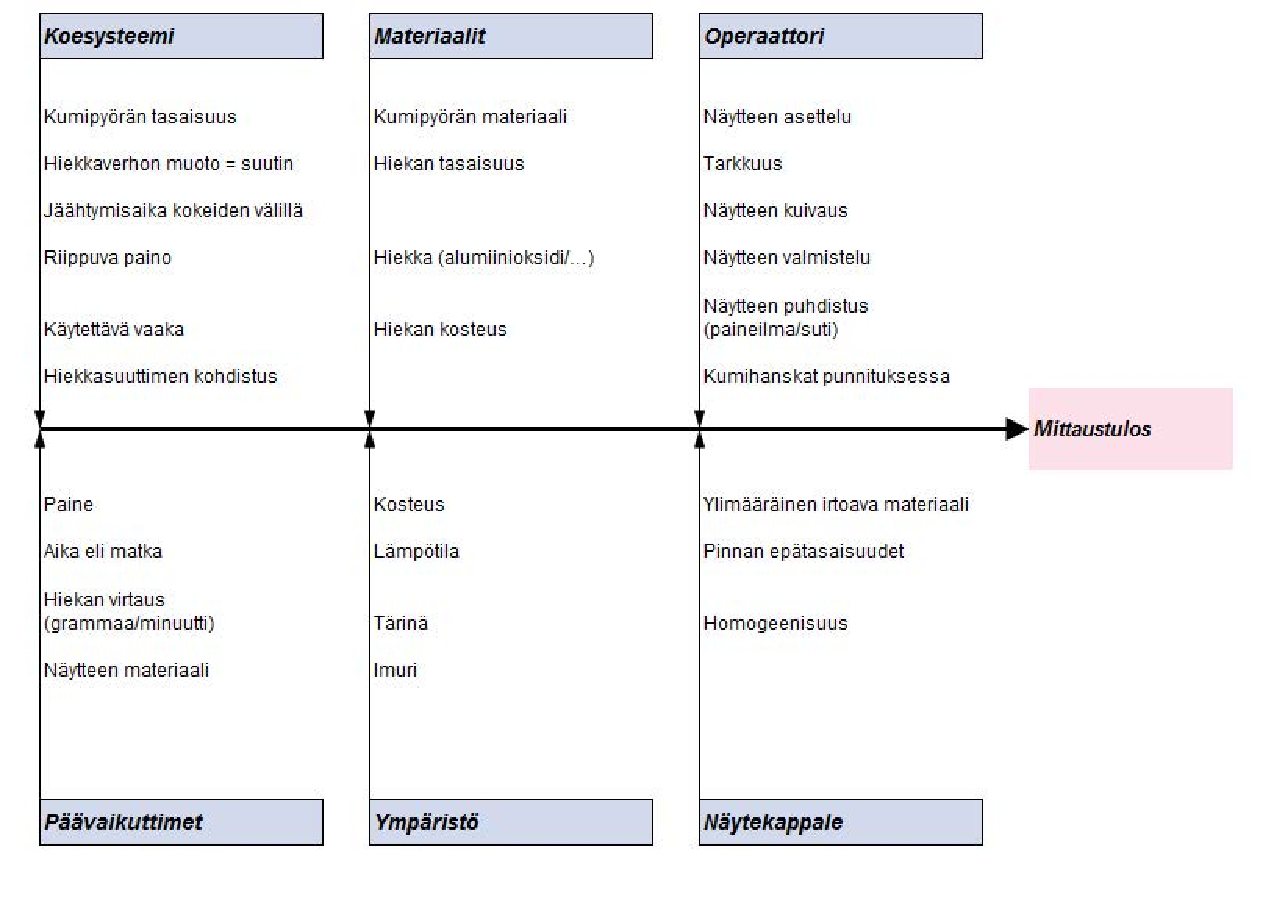
\includegraphics[width=1.0\textwidth]{Capture7}
  \end{center}
  \caption[Kalanruotokaavio abraasiokokeesta]{Arvio kokeessa vaikuttavista tekijöistä.}
  % Optional shorter caption in brackets is used in Table of Figures
  % (tof).
  \label{fig:ruoto1}
\end{figure}

\section{Tyypin 1 Mittajärjestelmäanalyysi}

Tyypin 1 mittajärjestelmäanalyysi toteutettiin valmistelemalla 10 näytekappaletta ja ajamalla jokaiseen satunnaisessa järjestyksessä 1 kulumisjälki, jonka jälkeen massahäviö mitattiin ja ajettiin samoihin näytteisiin toinen kulumisjälki, jälleen satunnaisessa järjestyksessä. Kumipyöränä käytettiin tällöin
normaalissa käytössä jo jonkin aikaa ollutta kumipyörää.
Kuva \ref{fig:t1grr} näyttää tulokset kokeiden ajojärjestyksessä, mittaustulokset y-akselilla on ilmoitettu milligrammoissa.

\begin{figure}
  \begin{center}
    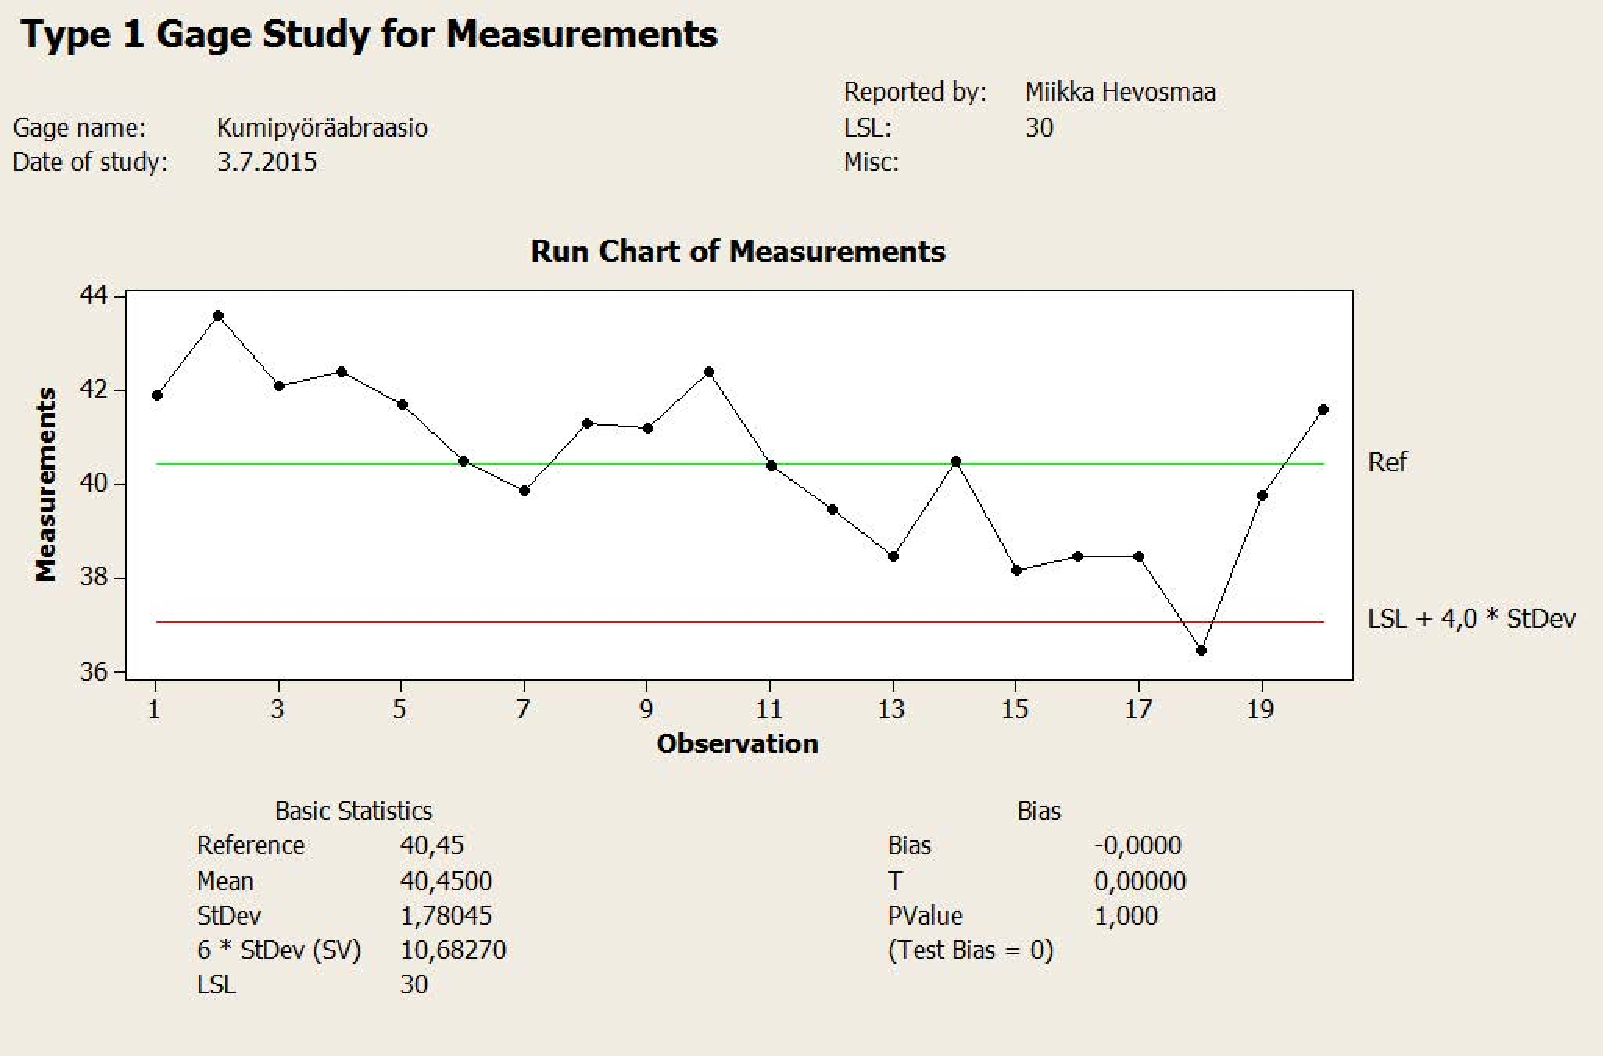
\includegraphics[width=1.0\textwidth]{t1grr}
  \end{center}
  \caption[Tulokset tyypin 1 mittajärjestelmäanalyysista]{Tulokset tyypin 1 mittajärjestelmäanalyysista.}
  % Optional shorter caption in brackets is used in Table of Figures
  % (tof).
  \label{fig:t1grr}
\end{figure}

Voidaan havaita hienoinen laskeva suuntaus mutta ainoastaan yksi koetulos on ohjelmiston laskeman (tilastollisesti merkittävän) punaisella merkityn alarajan alapuolella. Suuntaus voi hyvin olla kohinan tai pinnoitteen epähomogeenisuuden tuottama harha.
Koemäärä osoittautui myös liian pieneksi johtopäätösten tekemiseen.

Kuva \ref{fig:t1grr2} näyttää joka koekappaleen 2 testitulosta rinnakkain.
Epätavallista on että lähes jokaisen näytekappaleen massahäviö
laski toisella koekerralla. Syytä on vaikea arvella, mutta eräs
mahdollisuus on näytteiden keskeneräiseksi jäänyt kuivaaminen,
jonka johdosta nestettä haihtuisi vielä koetta edeltävän punnituksen
ja kokeen jälkeisen punnituksen välillä.

\begin{figure}
  \begin{center}
    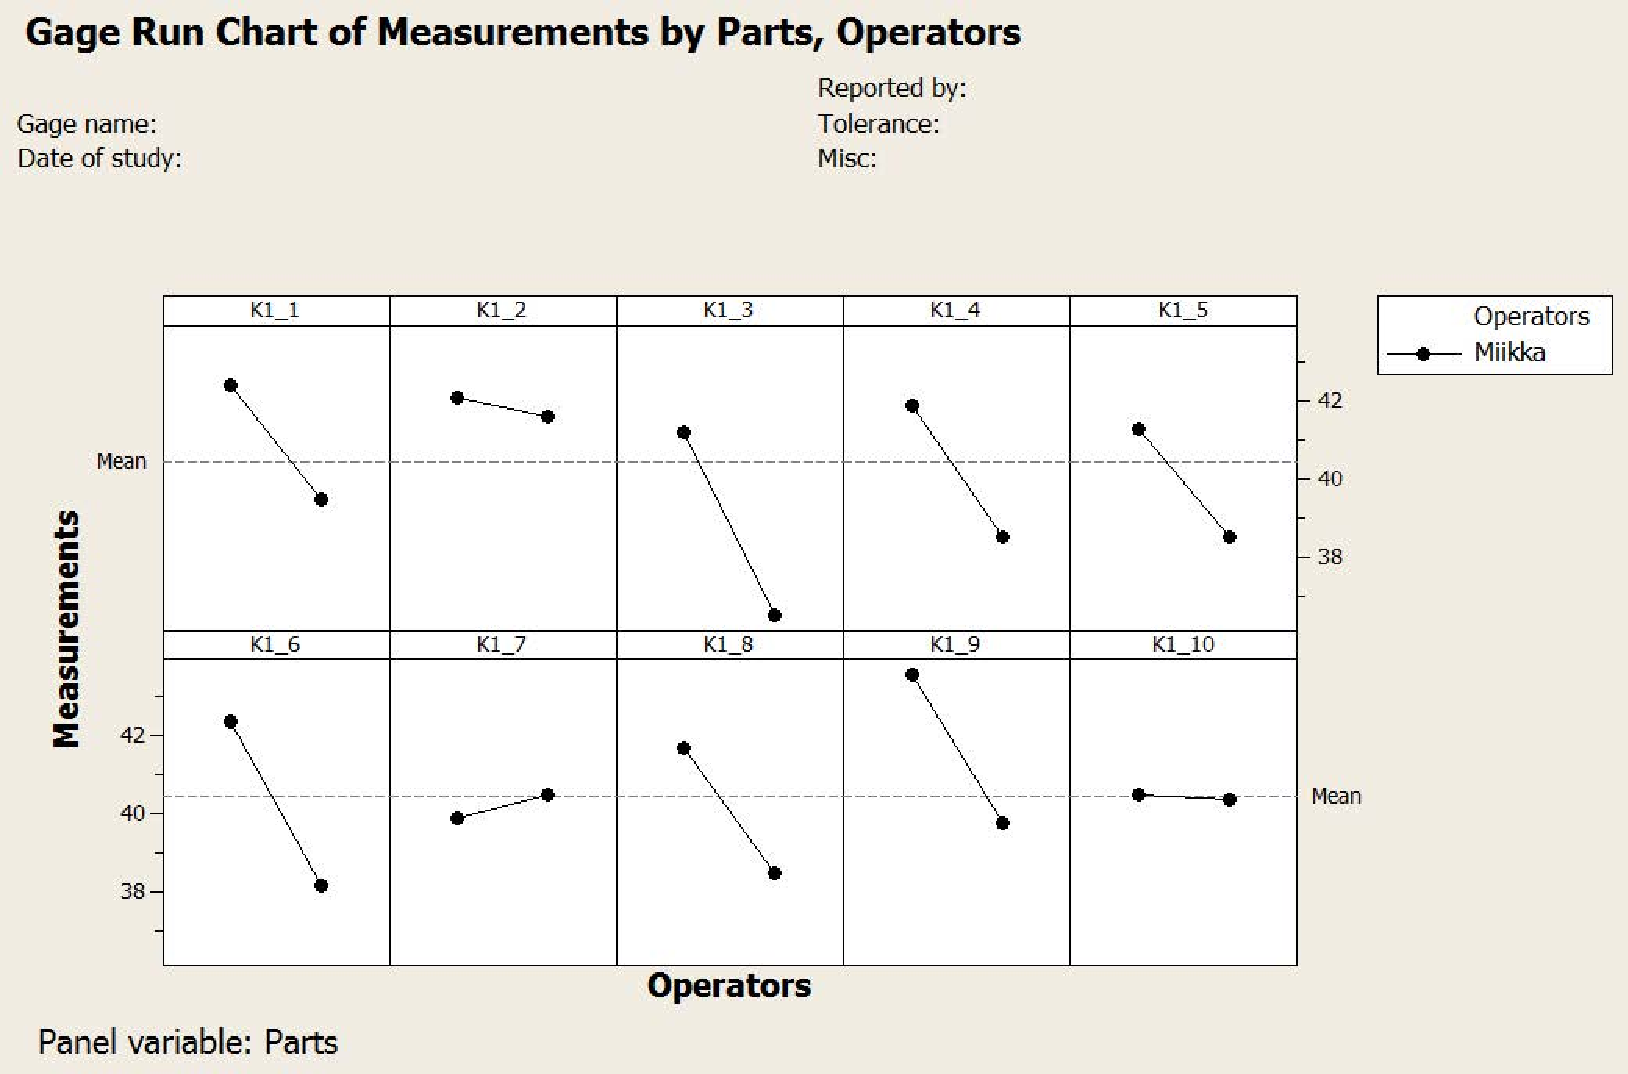
\includegraphics[width=1.0\textwidth]{t1grr2}
  \end{center}
  \caption[Rinnakkaiset tulokset tyypin 1 mittajärjestelmäanalyysista]{Tulokset tyypin 1 mittajärjestelmäanalyysista, saman koekappaleen tulokset rinnakkain.}
  % Optional shorter caption in brackets is used in Table of Figures
  % (tof).
  \label{fig:t1grr2}
\end{figure}


Koska koemäärä vaikutti riittämättömältä koetta jatkettiin valmistelemalla 6 näytekappaletta lisää ja ajamalla niihin kulumisjälki satunnaisessa järjestyksessä, mittaamalla massahäviöt ja ajamalla toinen kulumisjälki satunnaisessa järjestyksessä.
Kuva \ref{fig:t1grrjt} näyttää tuloksen kun uudet tulokset lisättiin kuvaan \ref{fig:t1grr}.
Hajonta vaikuttaa kaoottisemmalta ja laskeva suuntaus ei ole enää niin selvä. Näytteen ensimmäisen ja toisen mittaustuloksen vertailukuvaajaan lisättynä
tulos on kuvassa \ref{fig:t1grrjt2} (uudet näytteet merkittiin B-kirjaimella). 3:ssa uusista näytteistä massahäviö laski mutta 3:ssa myös nousi.
Aiempi ilmiö oli luultavasti sattumaa tai aiheutui tuntemattomasta virheestä koeprosessissa. Kaiken kaikkiaan tyypin 1 mittajärjestelmäanalyysi ei osoittanut testin olevan epästabiili, so. ajan suhteen muuttuva. Toisaalta on huomattava että 32 testiajoa n. 2 päivän aikana ei todennäköisesti ole riittävä määrä kokeita tai aikaa luotettavien tulosten saamiseksi.

\begin{figure}
  \begin{center}
    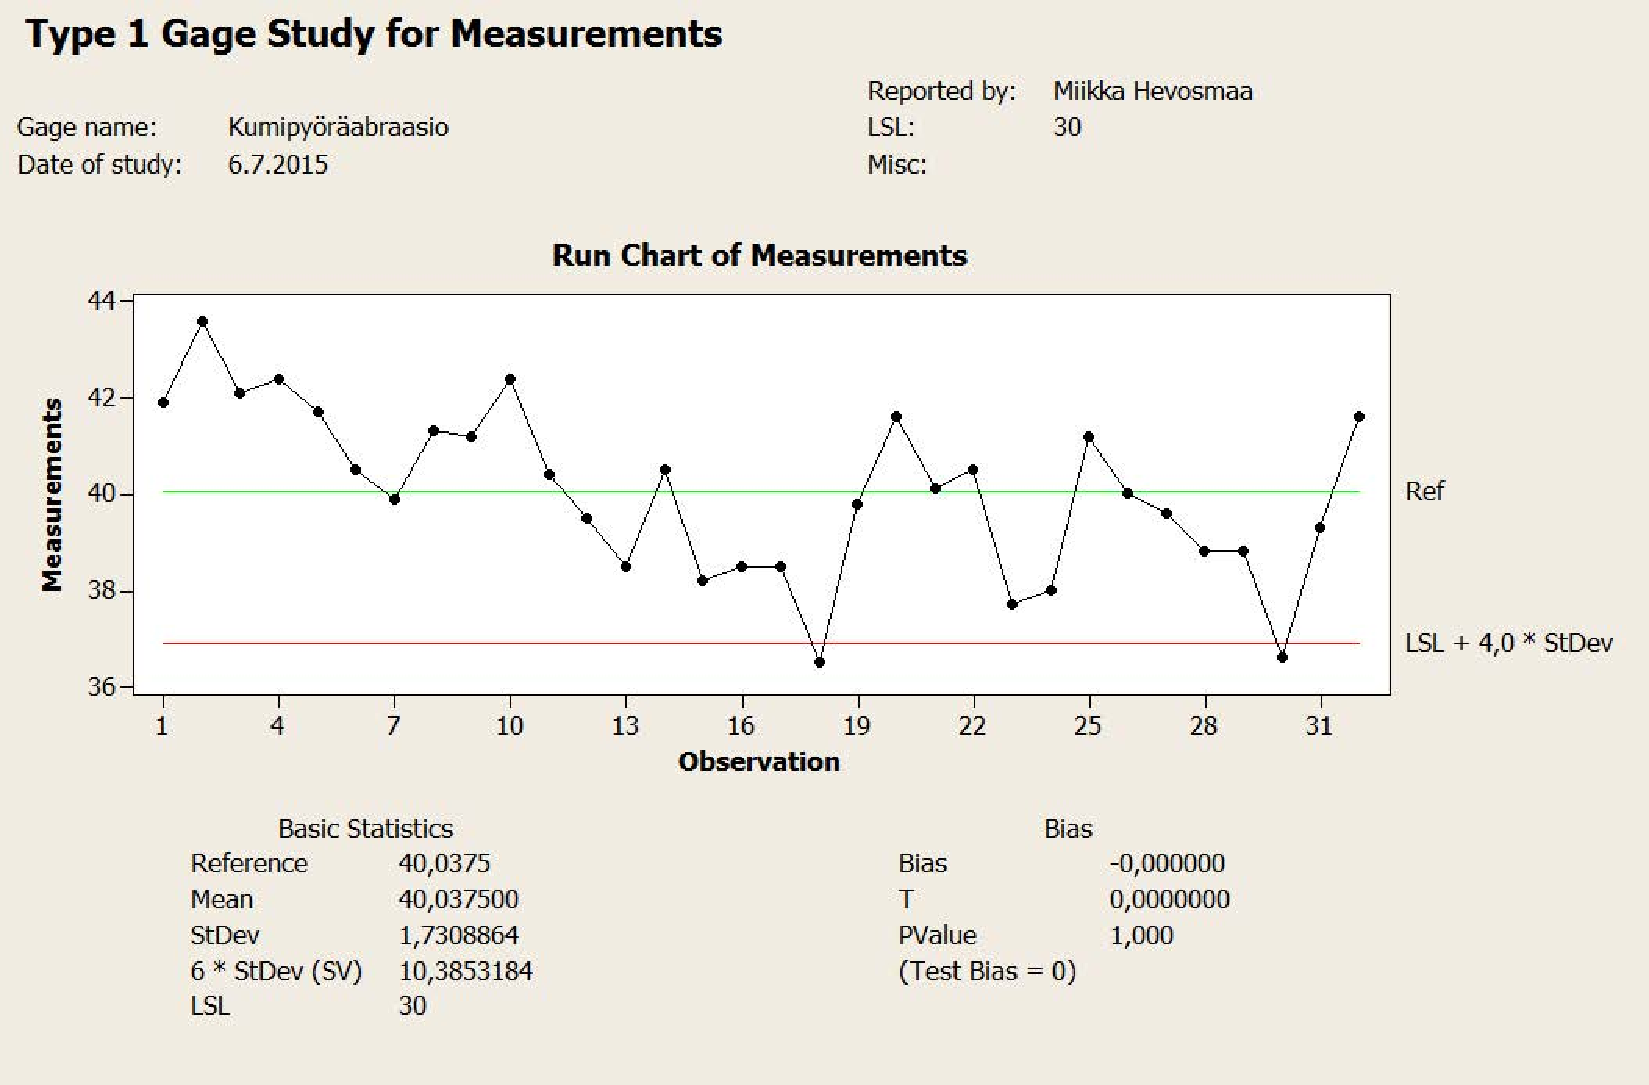
\includegraphics[width=1.0\textwidth]{t1grrjt}
  \end{center}
  \caption[Jatketun tyypin 1 mittajärjestelmäanalyysin tulokset]{Jatketun tyypin 1 mittajärjestelmäanalyysin tulokset.}
  % Optional shorter caption in brackets is used in Table of Figures
  % (tof).
  \label{fig:t1grrjt}
\end{figure}

\begin{figure}
  \begin{center}
    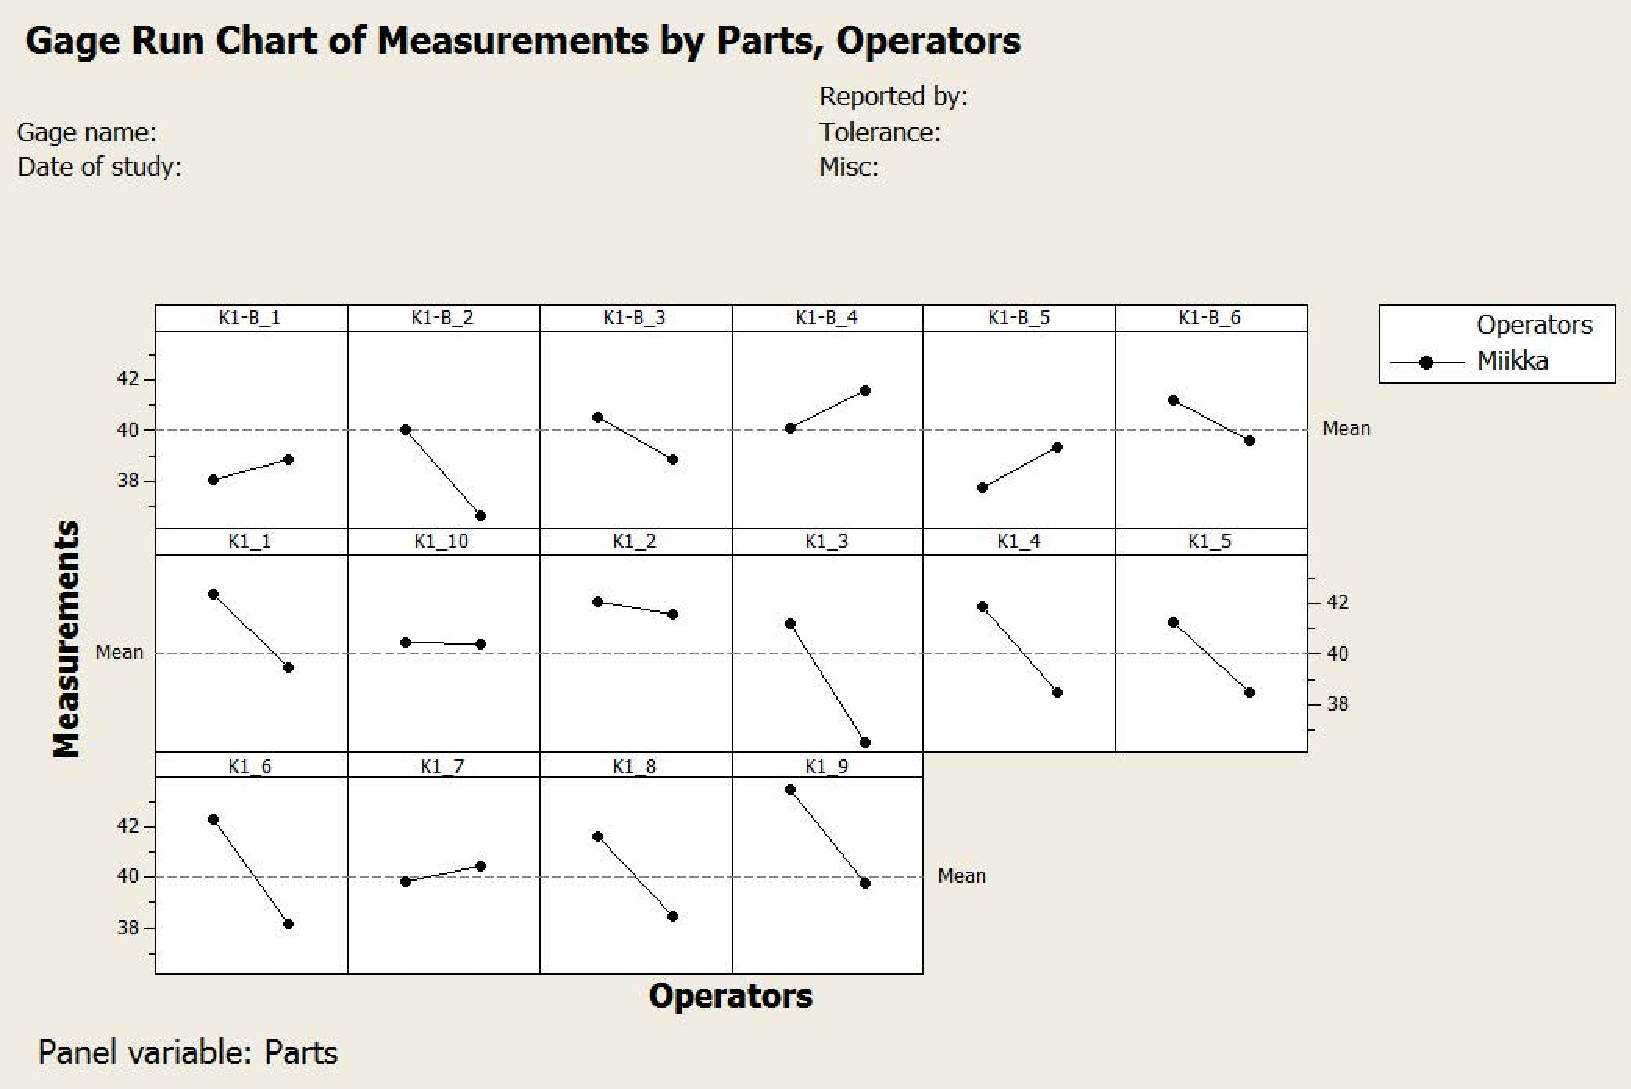
\includegraphics[width=1.0\textwidth]{t1grrjt2}
  \end{center}
  \caption[Jatketun tyypin 1 mittajärjestelmäanalyysin tulokset rinnakkain]{Jatketun tyypin 1 mittajärjestelmäanalyysin tulokset, saman koekappaleen tulokset rinnakkain. Uudet näytteet on merkitty B-kirjaimella.}
  % Optional shorter caption in brackets is used in Table of Figures
  % (tof).
  \label{fig:t1grrjt2}
\end{figure}

\section{Yleinen mittajärjestelmäanalyysi}

Mittajärjestelmäanalyysiin valitaan koekappaleita mahdollisimman kattavasti koko siitä valikoimasta joita mittajärjestelmä normaalissa käytössä kohtaisi, tarkoituksena vertailla tätä koekappaleiden odotettua hajontaa muihin hajontalähteisiin ja saada selville käyttäytyykö järjestelmä eri tavalla eri mittaustulosalueilla. Koekappaleita valmistettiin 12:sta eri pinnoitteesta jotka
numeroitiin 1 \ldots 12.
Eri käyttäjien sijasta käytettiin 3:a erilaista abraasiotestin kumipyörää koska tämän
uskottiin olevan merkittävästi todennäköisempi vaihtelun lähde kuin käyttäjän. Pyörät
valittiin seuraavasti:

\begin{description}
  \item[P1] Kumipyörä 1, normaalissa käytössä ollut kohtalaisesti kulunut kumipyörä
  \item[P2] Kumipyörä 2, sileä ja kulumaton kumipyörä
  \item[P3] Kumipyörä 3, keinotekoisesti hiomakoneella kulutettu kumipyörä, ”pompottava”
\end{description}

Koe tehtiin Minitab–ohjelman ohjeiden mukaan, hierarkkisena (nested) sillä kulumiskestävyyskoe on destruktiivinen eikä täsmälleen samaa näytekappaleen aluetta voi testata eri käyttäjillä/kumipyörillä. Onkin muistettava että kokeen taustalla on oletus pinnoitteiden homogeenisuudesta mikä ei välttämättä ole totuudenmukaista.

Joka pinnoitteesta valmisteltiin 3 näytekappaletta, joihin jokaiseen ajettiin 2 kulumisjälkeä. Aluksi laitteeseen asetettiin kumipyörä P1, jolla suoritettiin 1 koeajo jokaiseen eri pinnoitteeseen satunnaisessa järjestyksessä. Seuraavaksi asetettiin paikalleen kumipyörä P2 ja sama toistettiin uudelle joukolle näytekappaleita. Sama toistettiin jälleen pyörälle P3. Tämän jälkeen asetettiin paikalleen pyörä P1 uudelleen ja suoritettiin koeajo samoihin näytteisiin kuin oli suoritettu samalle pyörälle P1 aiemmin, jälleen satunnaisessa järjestyksessä. Näin tehtiin myös pyörälle P2 ja lopuksi pyörälle P3.

Minitabin varianssianalyysi tutkimuksesta on kuvassa \ref{fig:minitabgrr}.
\%Contribution (of VarComp) –kohdasta nähdään että pinnoitteiden erilaisuudesta johtuva varianssi on paljon suurempi kuin muista lähteistä aiheutuva (99,35 \% vs. 0,65 \%), joten koe kykenee ainakin erottamaan eri pinnoitteet toisistaan kumipyörien epäsäännöllisyydestä huolimatta. Projektin tavoitteiden kannalta kiinnostavampia ovat ehkä kuitenkin lukuisat kuvaajat joita tuloksista saadaan: Kuvassa \ref{subfig:ygrr1} nähdään kaikki koetulokset samassa graafissa, samaan näytekappaleeseen tehdyt eri koeajot ovat päällekkäin palloina ja yksiköt ovat milligrammoja.
Nähdään ainakin että mittaukset samalla pyörällä samalle pinnoitteelle ovat kohtuullisen lähellä toisiaan ja lähes kaikissa tapauksissa pystytään tunnistamaan samaksi pinnoitteeksi.

\begin{figure}
  \begin{center}
    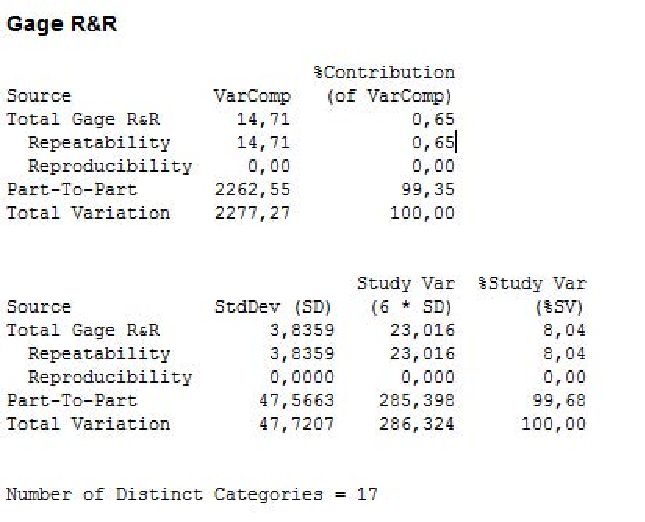
\includegraphics{minitabgrr}
  \end{center}
  \caption[Yleinen mittajärjestelmävarianssianalyysi]{Varianssianalyysi yleisen mittajärjestelmäanalyysin tuloksista.}
  % Optional shorter caption in brackets is used in Table of Figures
  % (tof).
  \label{fig:minitabgrr}
\end{figure}


Xbar–kuvaaja \ref{subfig:ygrrxbar} näyttää samaan kappaleeseen tehtyjen koeajojen keskiarvon joka pinnoitteelle ja kumipyörälle.
Voidaan jo nähdä että P1:n ja P2:n käyrien muodot ovat melko samanlaiset, ja P3:ssa referenssimateriaalin tulos on täysin erilainen. Kuvassa lähellä toisiaan olevat keskiarvo- ja ylä- ja alaraja-arvolinjat kertovat että koekappaleiden valinnat olivat onnistuneet sillä hajontaa oli paljon ja kaikki eivät asettuneet samoihin rajoihin.


Havainnollisin kuvaaja on R-chart –käyrä, kuva \ref{subfig:ygrrrchart}. Käyrä näyttää eron samaan koekappaleeseen tehdyn kahden eri kokeen välillä. Jos pinnoitteet oletetaan homogeenisiksi, on paras kumipyörä sellainen, joka tuottaa mahdollisimman pienen eron koeajoihin.
Kuvasta nähdään että johdonmukaisimpia tuloksia antaa sileä, uusi kumipyörä nro 2. Eniten vaihtelevat epätasaisen kumipyörä 3:n tulokset. Voidaan todeta että epätasainen, ”pompottava” kumipyörä voi aiheuttaa yli 10 milligramman eroja saman pinnoitteen koetuloksille.


\begin{figure*}
  \begin{center}
    \subfigure[Yleisen mittajärjestelmäanalyysin tulokset samassa graafissa.]{
      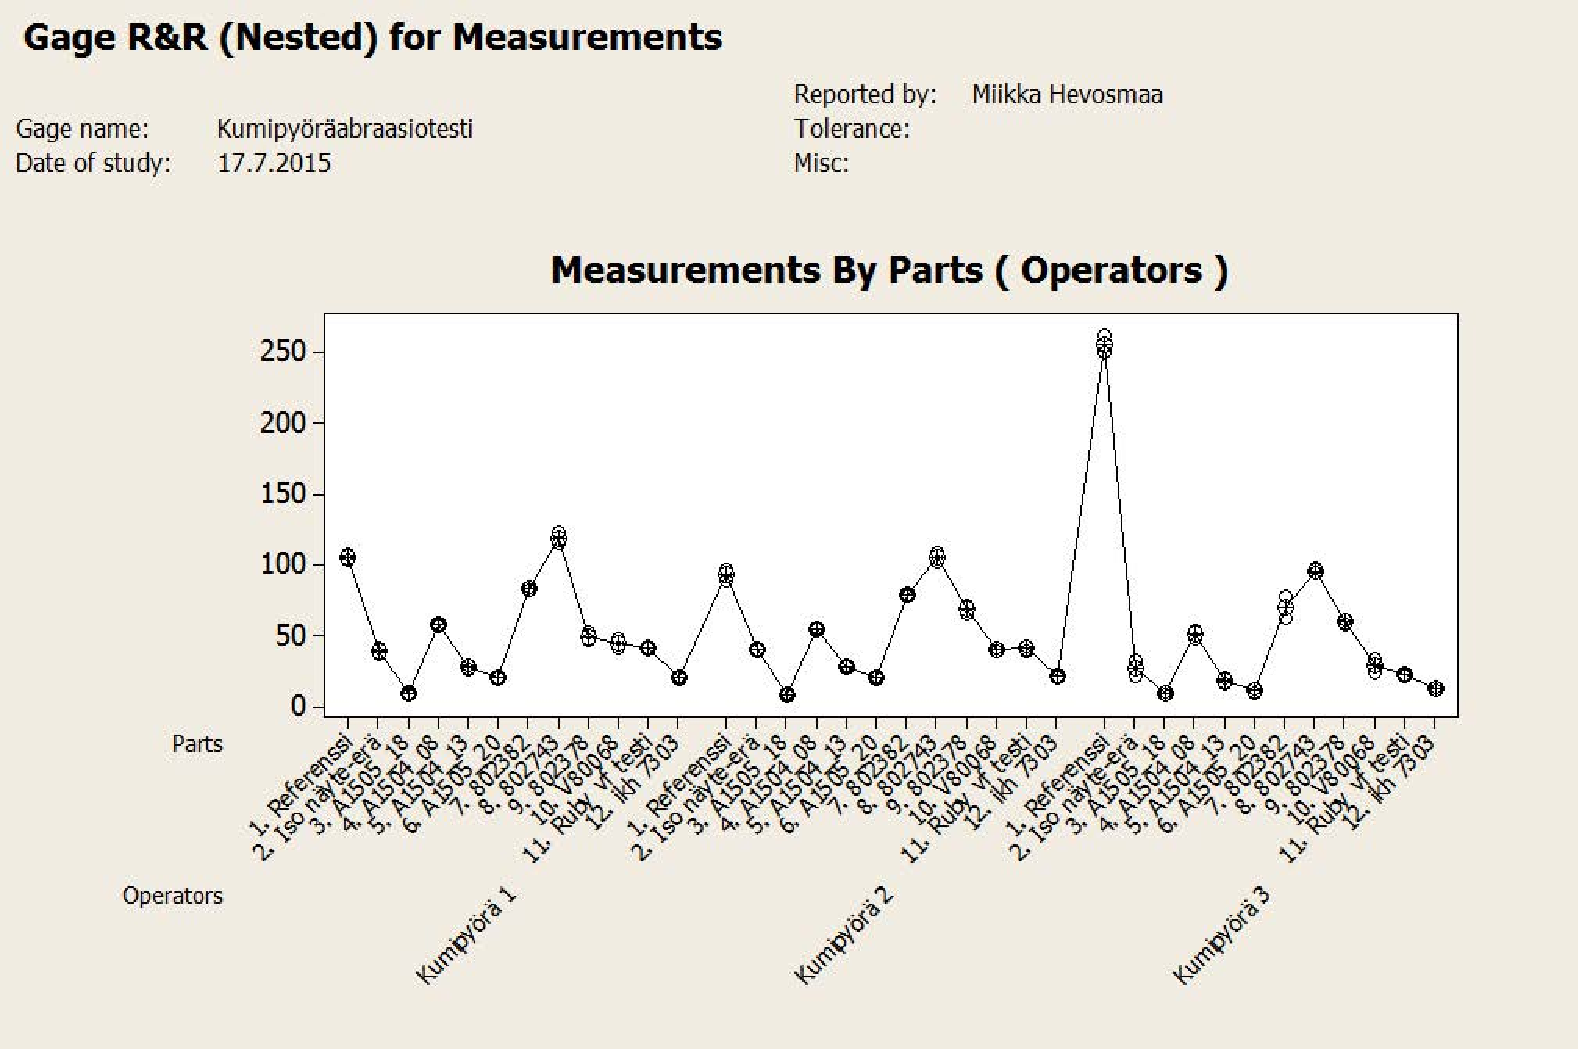
\includegraphics[width=\textwidth]{ygrr1}
      \label{subfig:ygrr1}}
    %\qquad                        % i) Ugly hack to get more horizontal space between figures
    %\hspace{0.05\textwidth}      % ii) Another ugly way to hack space
    % ~~                          % iii) Yet another...

    \subfigure[Yleisen mittajärjestelmäanalyysin Xbar-kuvaaja.]{
      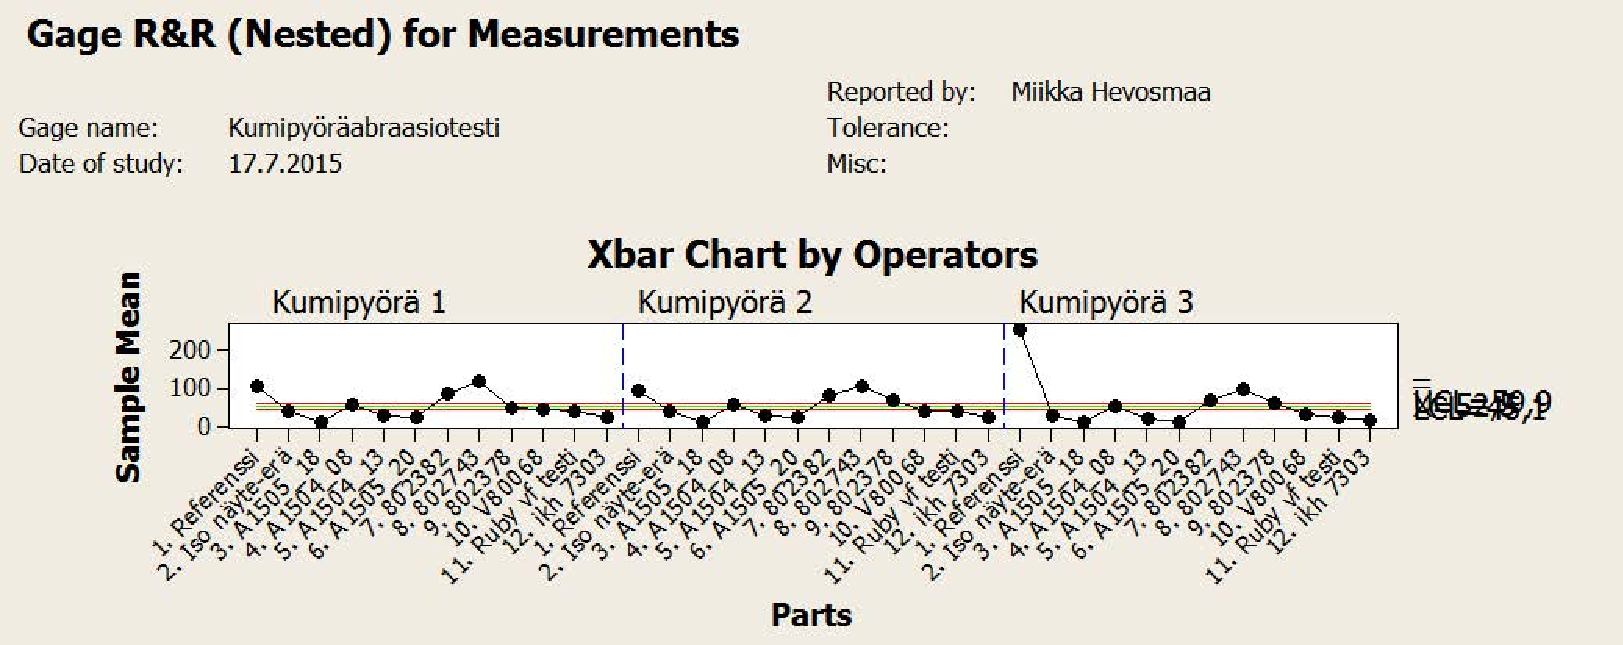
\includegraphics[width=\textwidth]{ygrrxbar}
      \label{subfig:ygrrxbar}}

    \subfigure[Yleisen mittajärjestelmäanalyysin R-chart -kuvaaja.]{
      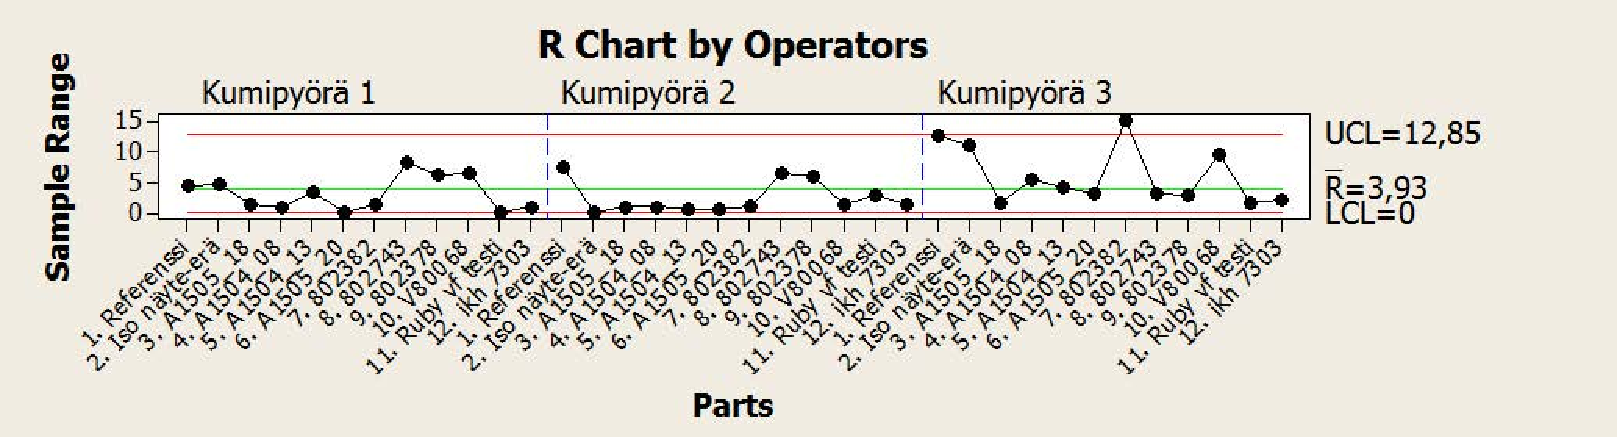
\includegraphics[width=\textwidth]{ygrrrchart}
      \label{subfig:ygrrrchart}}
    \caption[Yleisen mittajärjestelmäanalyysin tulokset]{Yleisen mittajärjestelmäanalyysin tulokset.}
    % Optional shorter caption in brackets is used in Table of Figures
    % (tof).

    \label{fig:ygrr}
  \end{center}
\end{figure*}



Kuva \ref{fig:ygrr2} näyttää saman kappaleen ensimmäisen ja toisen koeajon rinnakkain, sekä saman pinnoitteen tulokset eri kumipyörillä rinnakkain.
Vaikka yleensä tulokset osuvat lähimain samalle alueelle eri kumipyörilläkin, ainakin yksi materiaali reagoi täysin eri tavalla kumipyörä nro 3:lle: teräksinen referenssimateriaali. Tämä kertoo että ainakin jotkin materiaalit voivat olla herkempiä pyörän epätasaisuudelle kuin toiset. Luonnollisesti ei ole toivottavaa että referenssimateriaali, jolla koelaitteiston toimintaa seurataan, reagoi eri parametreihin eri tavalla kuin varsinaisesti testattavat pinnoitteet. Toisaalta herkempi referenssimateriaali voi olla hyvä indikaattori joka varoittaa kuluneesta kumipyörästä ajoissa.

\begin{figure}
  \begin{center}
    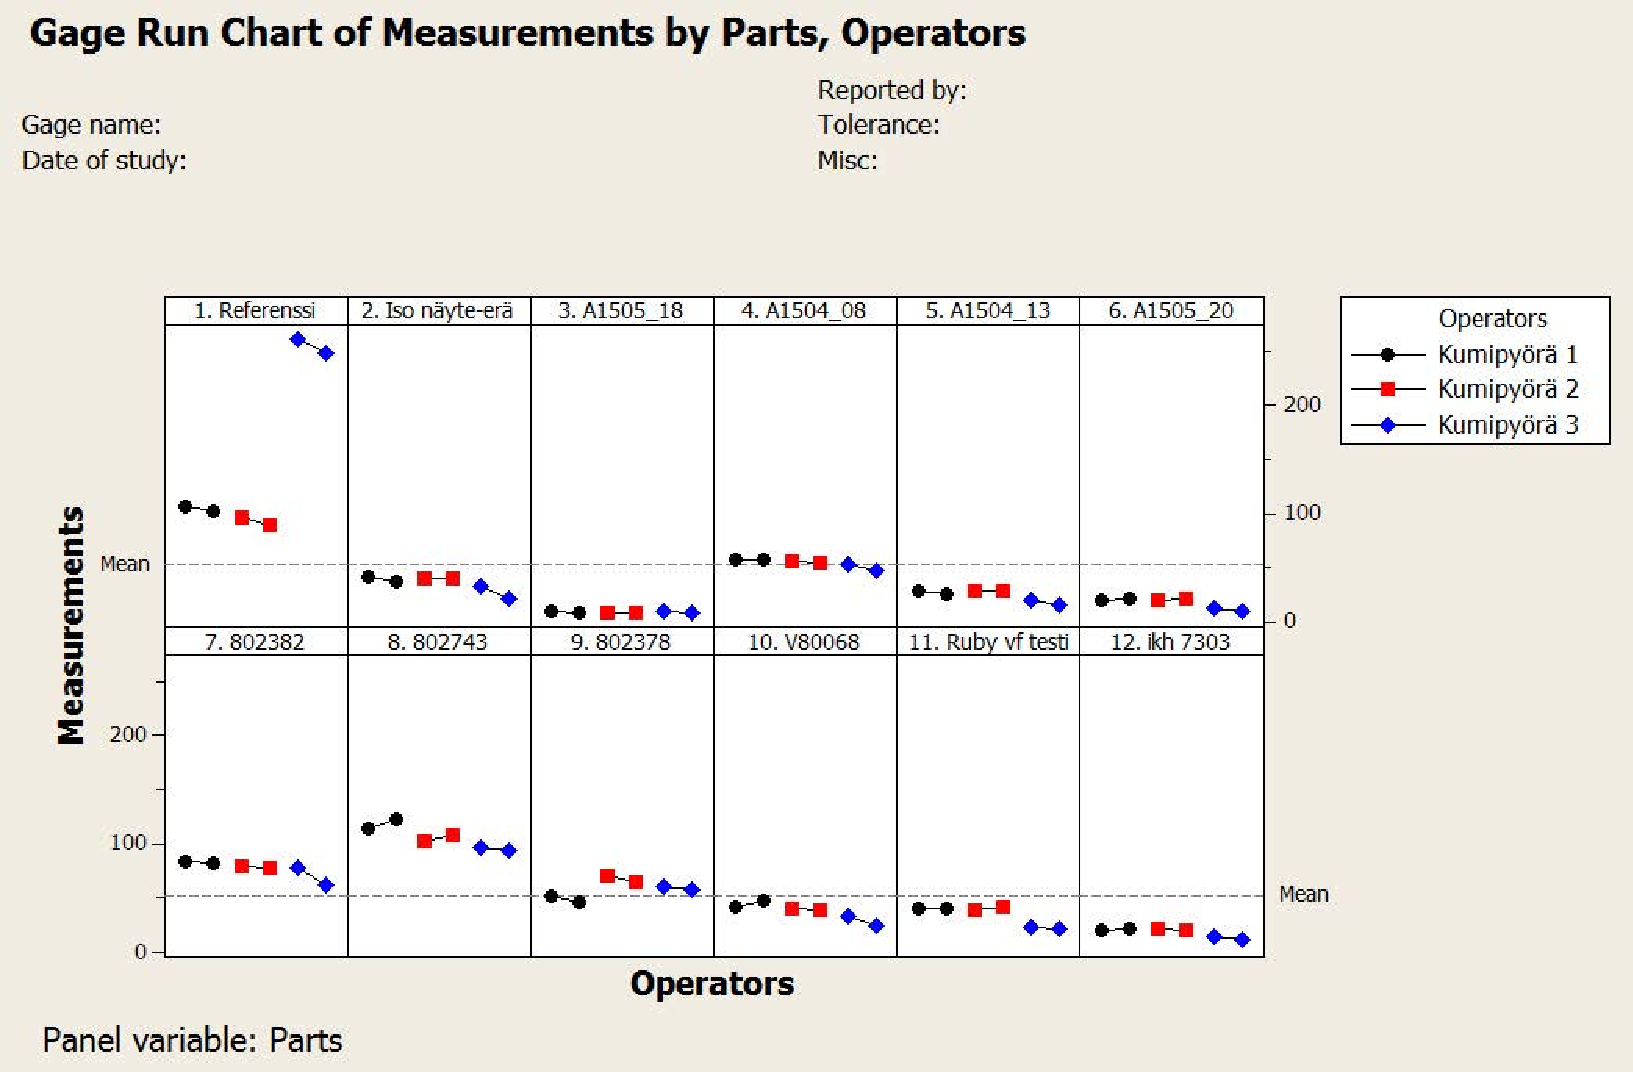
\includegraphics[width=1.0\textwidth]{ygrr2}
  \end{center}
  \caption[Yleinen mittajärjestelmäanalyysi: Rinnakkaiset tulokset]{Tulokset yleisestä mittajärjestelmäanalyysista, saman koekappaleen tulokset rinnakkain.}
  % Optional shorter caption in brackets is used in Table of Figures
  % (tof).
  \label{fig:ygrr2}
\end{figure}






Kaiken kaikkiaan mittajärjestelmäanalyysi paljasti että kumipyörän epätasaisuudella on havaittava vaikutus mittaustuloksiin, tosin verrattuna eri pinnoitteiden välisiin eroihin tämä vaikutus ei ole suuri, paitsi referenssimateriaalin tapauksessa. Kulunut pyörä antaa vaihtelevampia tuloksia samalle materiaalille.

\section{Muut varianssianalyysit}

Kumipyörän epätasaisuuden osoittauduttua suhteellisen pieneksi osaksi hajontaa tutkittiin muita mahdollisia syitä vaihteleville tuloksille.
Päädyttiin siihen johtopäätökseen että vaihteleviin tuloksiin luultavimmin vaikuttavat näytteen kunnollinen kuivaus, kumipyörän kovuuden vaihtelu, hiekan virtausmäärän vaihtelu ja hiekan kasaantuminen ja epätasainen virtaus näytekappaleen päältä. Näytteiden kuivaus vaikutti epätodennäköiseltä syyltä sillä kuivumiseen annettiin aina reilusti aikaa, ainakin seuraavaan päivään asti, ja kuivausmenetelmää oli käyttänyt kokenut operaattori, joka ei ollut maininnut kuivauksessa olleen mitään vaikeuksia. Hiekan virtausmäärä vaikutti vakiolta aina ennen laitteen käyttämistä tehdyssä mittauksessa, lähes aina ~60 g/min. Kumipyörän kovuuden vaihtelun mittaaminen osoittautui vaikeaksi, käsin käytettävän Shore –durometrin mittaustulokset olivat vaihtelevia ja vaikeita toistaa.

Hiekan oli havaittu kasautuvan epäsäännölliseen muotoon näytekappaleen päälle ja vasta siitä laskeutuvan
kumipyörän ja näytteen väliseen rakoon. Vaikutti järkeenkäyvältä että tällainen epätasainen virtaus vaikuttaisi koetulosten hajontaan. Standardissa G65 \parencite{Standard2010}
ja muissa kumipyöräabraasiolaitteen kaaviokuvissa hiekkaverho putosi aina suoraan pyörän ja kappaleen väliseen rakoon. Vaikutusta olisi myös helppo tutkia, oli vain valmistettava näytekappaleita jotka olivat niin korkeita että niiden yläreuna olisi korkeammalla kuin hiekkasuuttimen pää, jolloin hiekka ei pääsisi kasaantumaan reunan päälle.
Valittiin 8 kpl hyväpintaisia 100 x 50 mm koekappaleita, joista 4 leikattiin 50 x 50 mm muotoisiksi
kuten kuvassa \ref{fig:kappaleet}.
100 x 50 mm kappaleista hiottiin kulmat pois, koska muuten ne ottivat kiinni hiekkasuuttimen päähän kokeen aikana.

\begin{figure}
  \begin{center}
    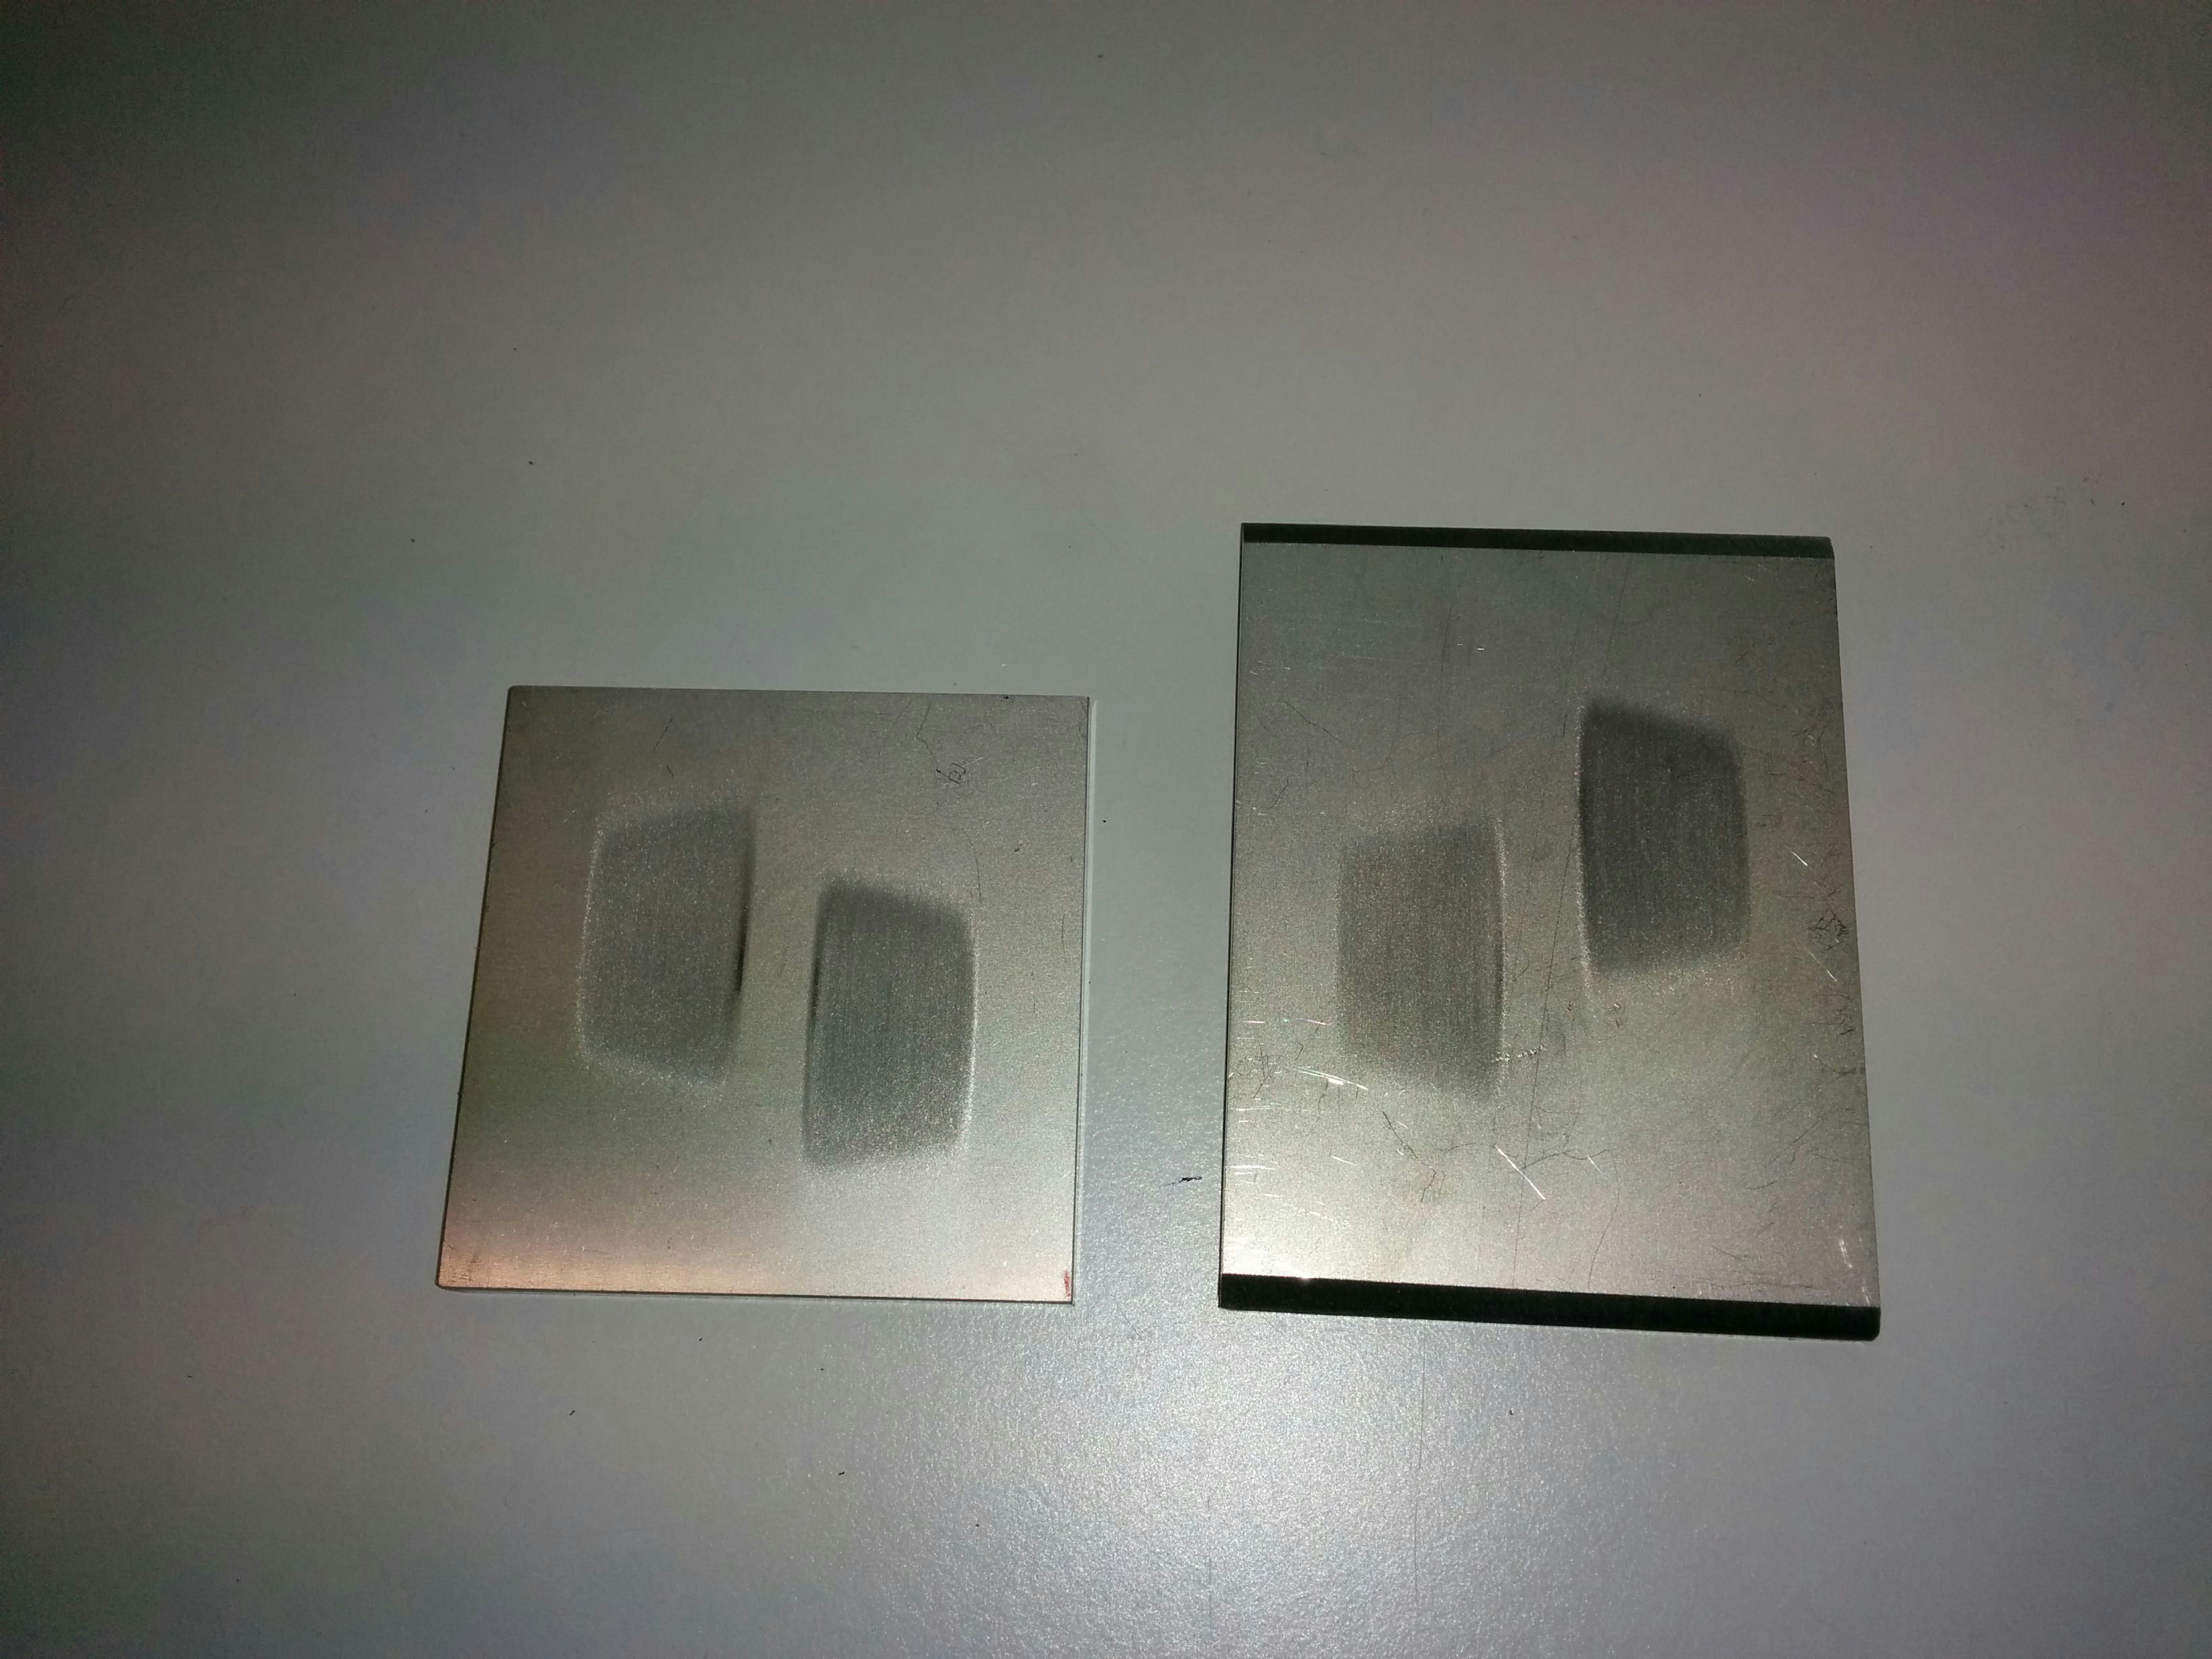
\includegraphics[width=0.7\textwidth]{kappaleet}
  \end{center}
  \caption[Virtauskokeen koekappaleita]{Hiekan epätasaisen virtauksen tutkimiseen valmistettuja koekappaleita.}
  % Optional shorter caption in brackets is used in Table of Figures
  % (tof).
  \label{fig:kappaleet}
\end{figure}

Varianssianalyysi suoritettiin hierarkkisena Gage R\&R:nä, kuten aiempikin mittajärjestelmäanalyysi. Ensin jokaiseen neliönmuotoiseen kappaleeseen ajettiin koe satunnaisessa järjestyksessä, sitten jokaiseen suorakulmion muotoiseen, sen jälkeen toinen koeajo samoihin neliökappaleisiin, ja sama suorakulmioihin. Kokeissa käytettiin edellisessä kokeessa luotettavimmaksi osoittautunutta kumipyörä P2:ta. Minitab tuotti
kuvan \ref{subfig:virtausxbar} mukaisen Xbar –kuvaajan ja kuvan \ref{subfig:virtausrchart} mukaisen R-chart-kuvaajan.
Kuvasta nähdään että suorakulmion muotoisilla näytteillä, joissa hiekan virtaus on hallitumpaa, saman kappaleen eri mittausten välillä on vähemmän eroa. Yksiköt ovat jälleen milligrammoja.
Koeajojen rinnakkainen vertaus on kuvassa \ref{subfig:virtausrinnakkaiset}
Odottamattomasti jokaisen 50 x 50 mm –näytteen massahäviö laski toisella koeajolla mutta vastaavaa ilmiötä ei esiintynyt 100 x 50 mm –näytteillä.

\begin{figure*}
  \begin{center}
    \subfigure[Hiekan epätasaisen virtauksen kokeen Xbar-kuvaaja.]{
      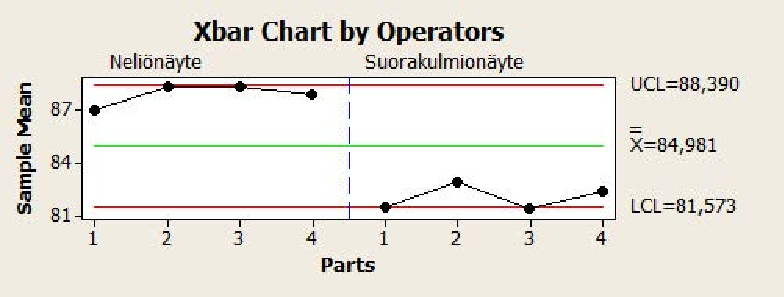
\includegraphics[width=\textwidth]{virtausxbar}
      \label{subfig:virtausxbar}}
    %\qquad                        % i) Ugly hack to get more horizontal space between figures
    %\hspace{0.05\textwidth}      % ii) Another ugly way to hack space
    % ~~                          % iii) Yet another...

    \subfigure[Hiekan epätasaisen virtauksen kokeen R-chart-kuvaaja]{
      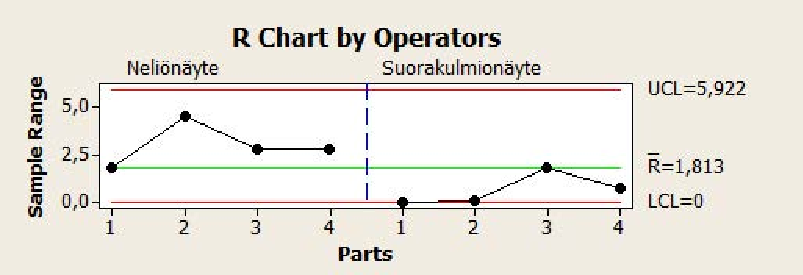
\includegraphics[width=\textwidth]{virtausrchart}
      \label{subfig:virtausrchart}}

    \subfigure[Hiekan epätasaisen virtauksen kokeen tulokset, saman koekappaleen tulokset esitettynä rinnakkain]{
      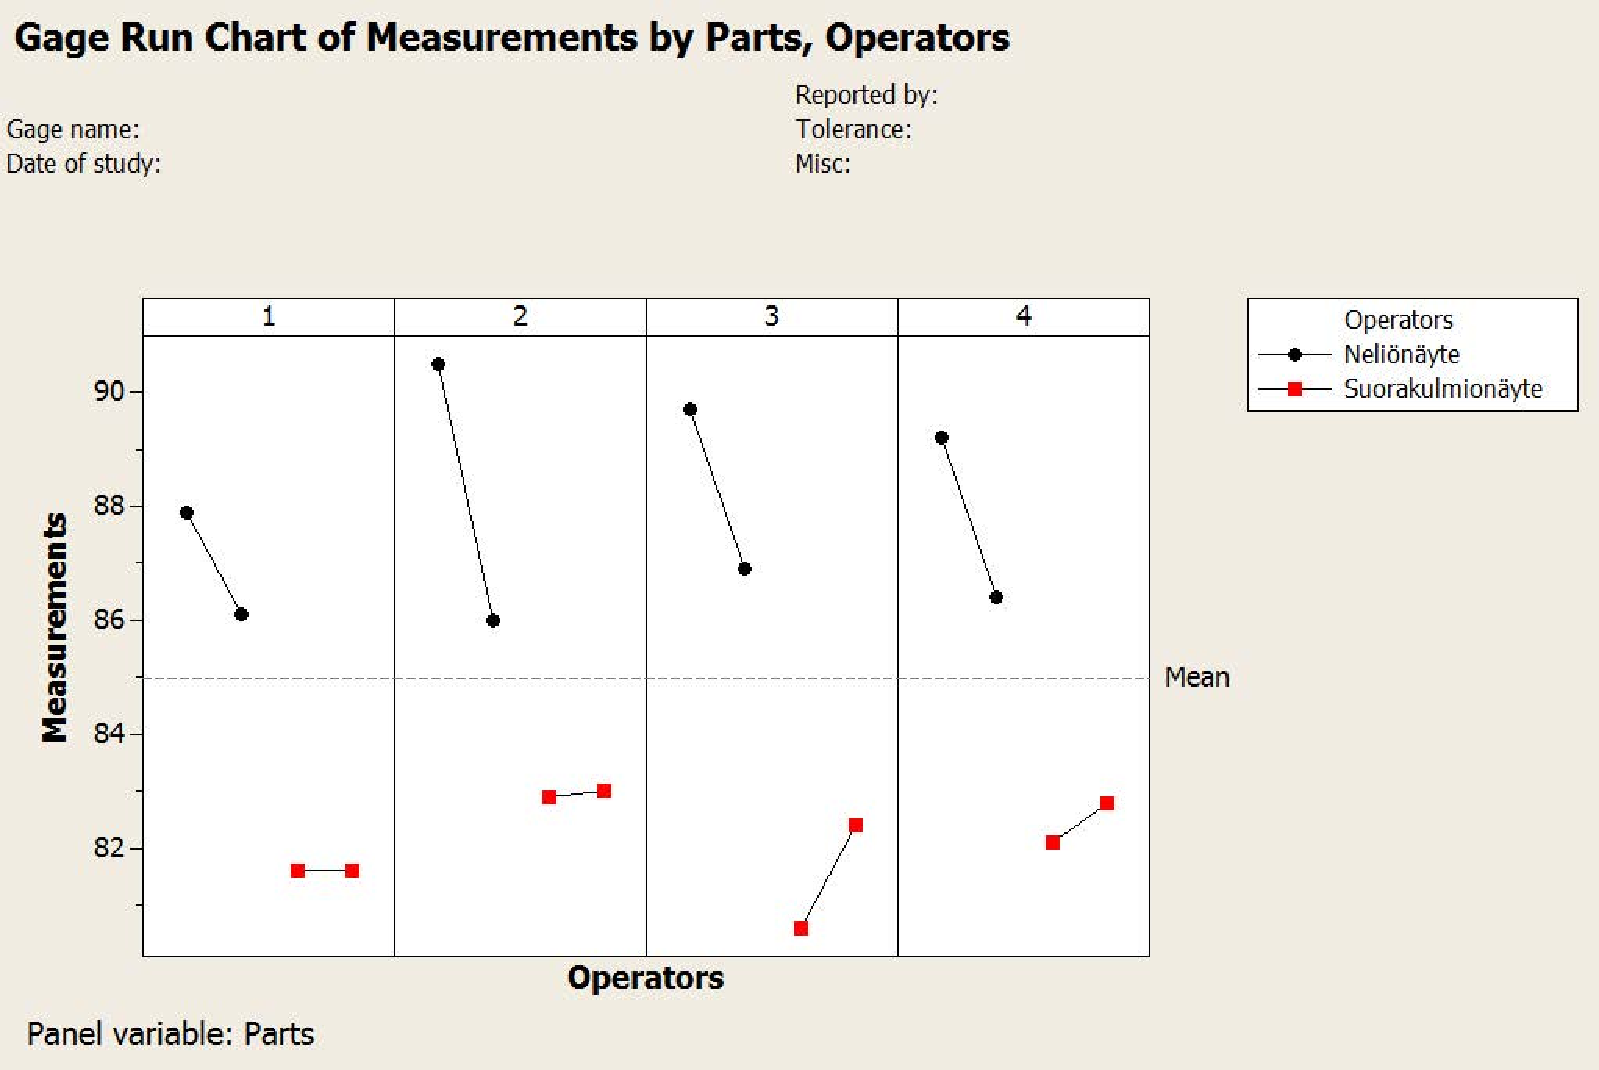
\includegraphics[width=\textwidth]{virtausrinnakkaiset}
      \label{subfig:virtausrinnakkaiset}}
    \caption[Virtauskokeen tulokset]{Hiekan epätasaisen virtauksen tutkimuksen tulokset.}
    % Optional shorter caption in brackets is used in Table of Figures
    % (tof).

    \label{fig:virtauskoe}
  \end{center}
\end{figure*}


Näitten tulosten ansiosta päätettiin toistaa sama hiekan virtauksen varianssianalyysi suuren projektia varten tehdyn näyte-erän karbidipinnoitteille. Tästä erästä leikattiin pieni ”kansi”, joka asetettiin näytteen päälle näytteenpidikkeeseen, kuten kuvassa \ref{fig:kappaleet2}
Kuvassa \ref{fig:kpllaitteessa} näkyvä pieni pahvinpala piti kannen tiukasti paikoillaan kokeen aikana.
Muuten koe suoritettiin samoin kuin edellinen teräskappaleilla tehty koe,
eli hierarkkisena Gage R\&R:nä.
Syntynyt Xbar –kuvaaja on kuvassa \ref{subfig:virtaus2xbar}, R-chart kuvassa \ref{subfig:virtaus2rchart} ja rinnakkaistarkastelu
kuvassa \ref{subfig:virtaus2rinnakkaiset}.

\begin{figure}
  \begin{center}
    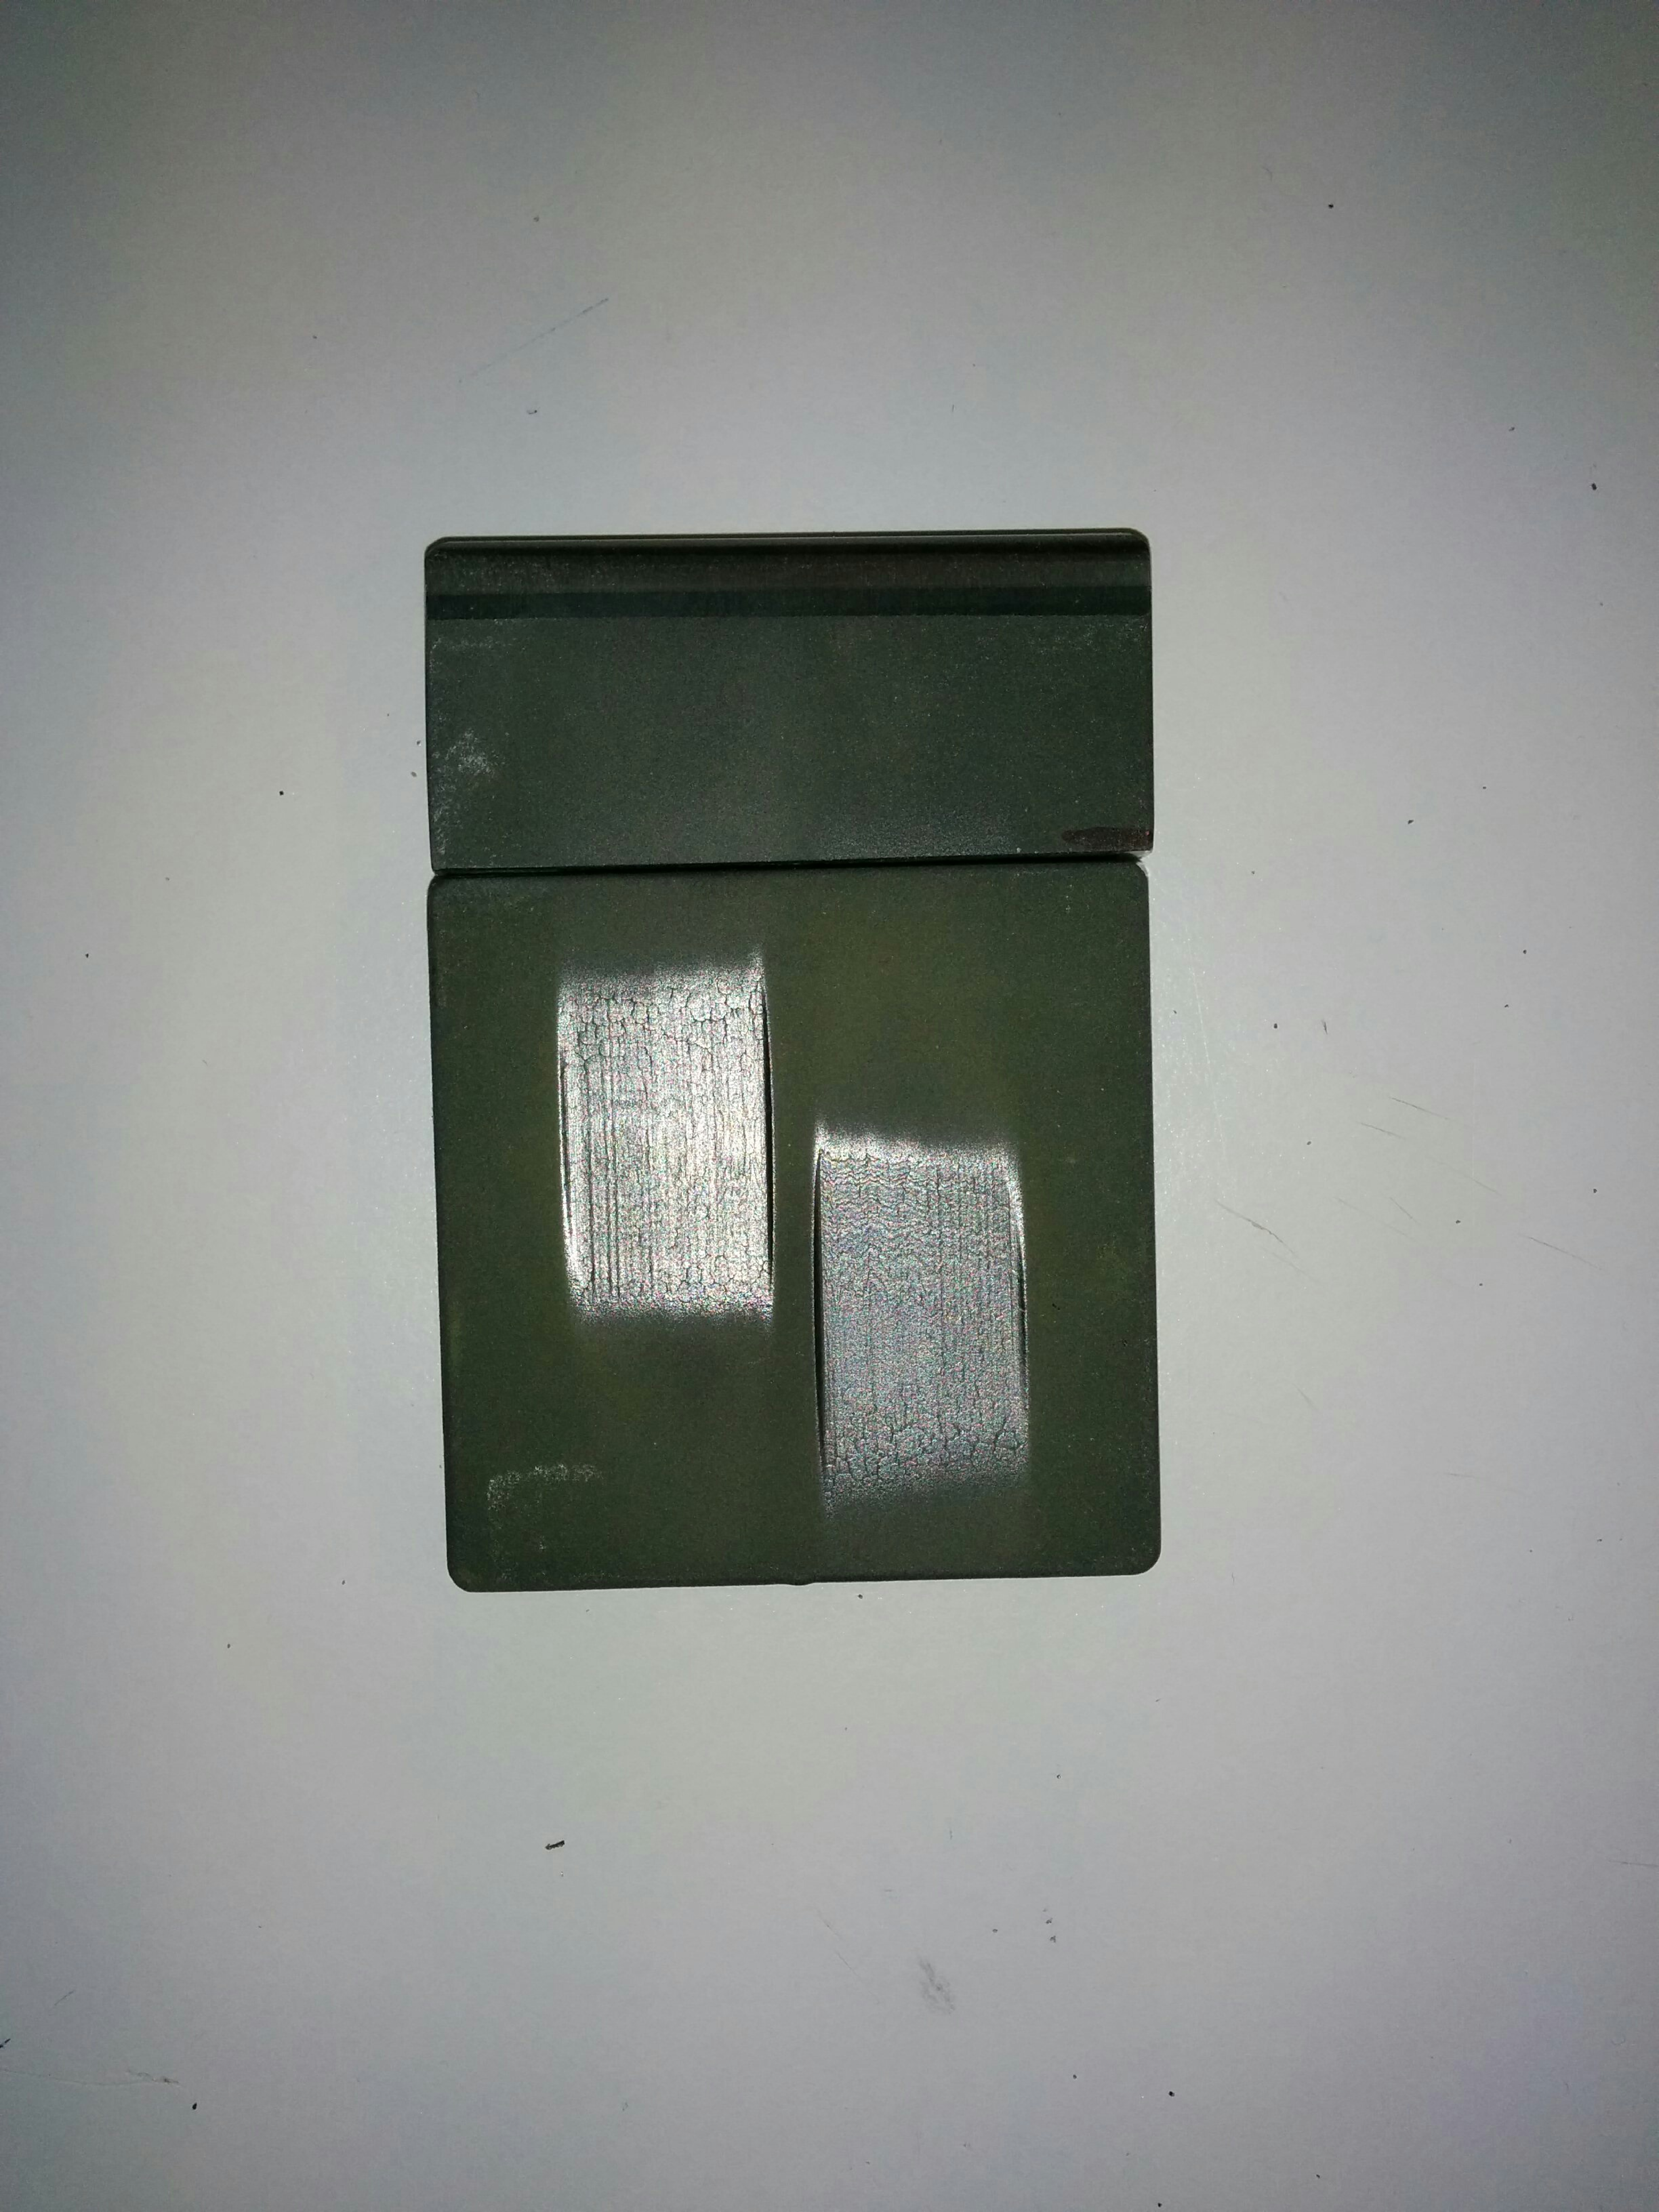
\includegraphics[width=0.7\textwidth]{kappaleet2}
  \end{center}
  \caption[Toisen virtauskokeen koekappaleita]{Hiekan epätasaisen virtauksen tutkimiseen valmistettuja karbidipinnoitteisia koekappaleita.}
  % Optional shorter caption in brackets is used in Table of Figures
  % (tof).
  \label{fig:kappaleet2}
\end{figure}

\begin{figure}
  \begin{center}
    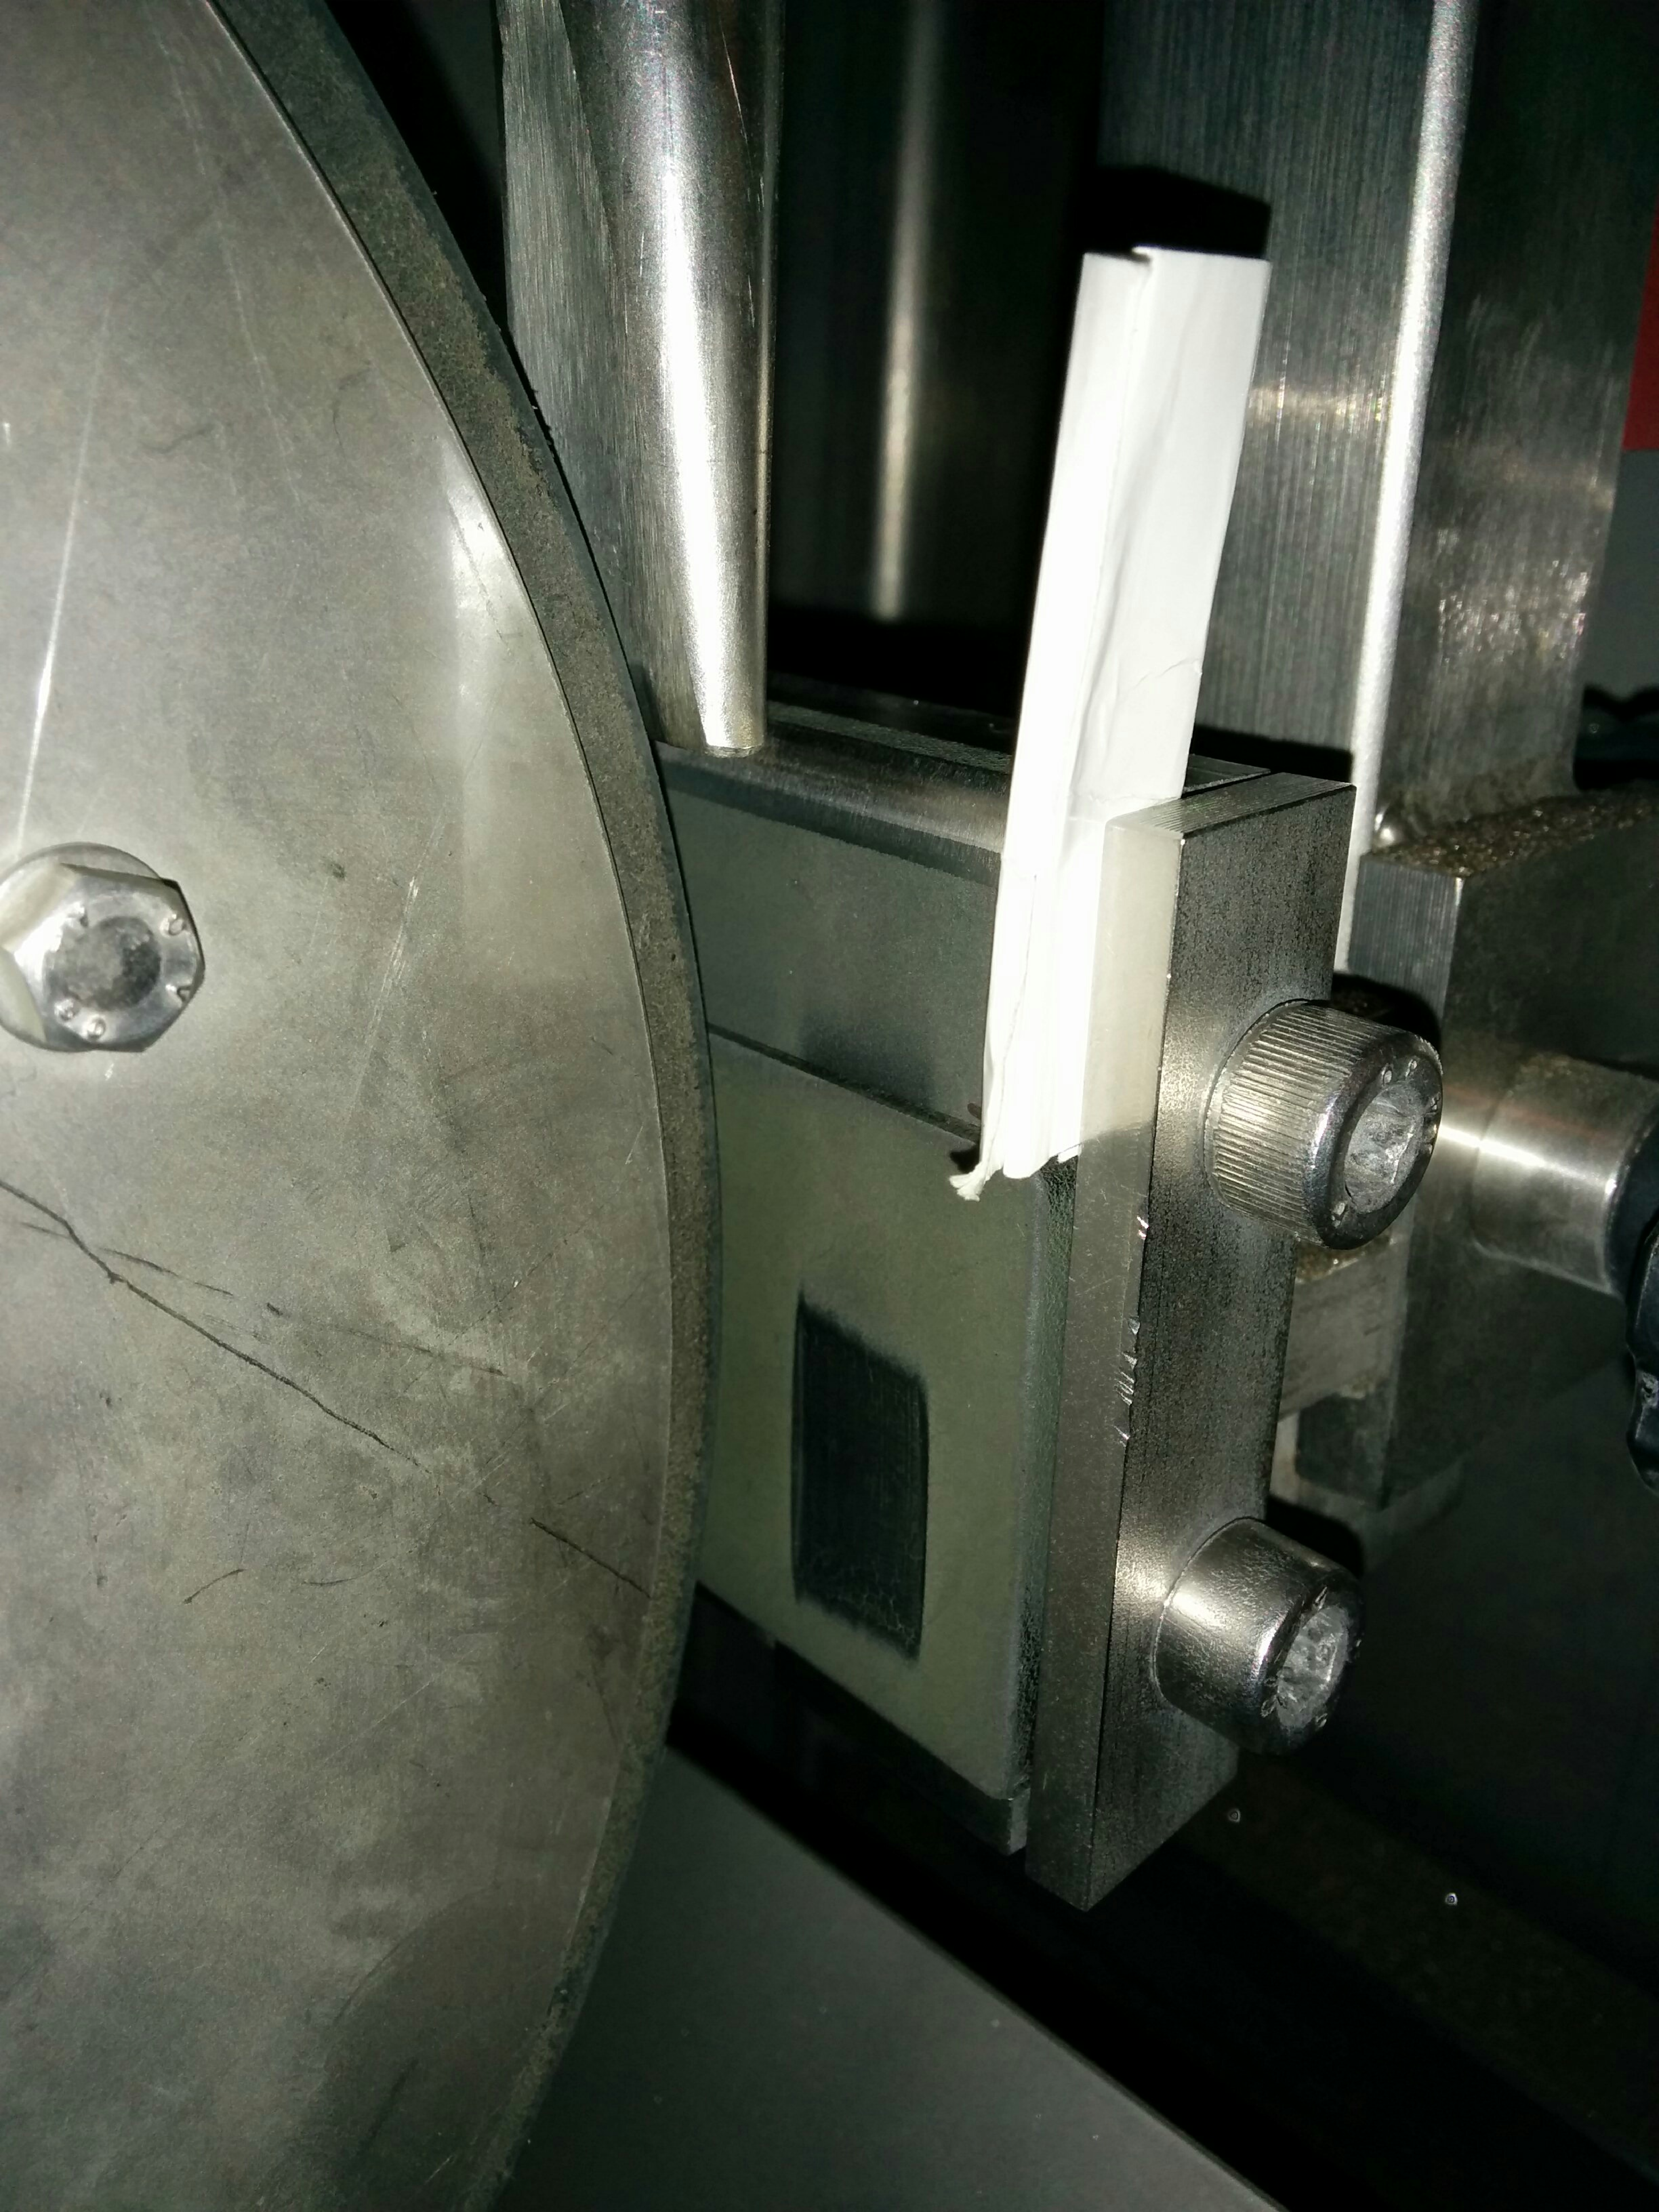
\includegraphics[width=0.7\textwidth]{kpllaitteessa}
  \end{center}
  \caption[Toisen virtauskokeen koejärjestely]{Toisen virtauskokeen koekappale, koekappaleen "kansi" ja "kantta" paikallaan pitävä pahvinpala koelaitteessa.}
  % Optional shorter caption in brackets is used in Table of Figures
  % (tof).
  \label{fig:kpllaitteessa}
\end{figure}

\begin{figure*}
  \begin{center}
    \subfigure[Toisen epätasaisen virtauksen kokeen Xbar-kuvaaja.]{
      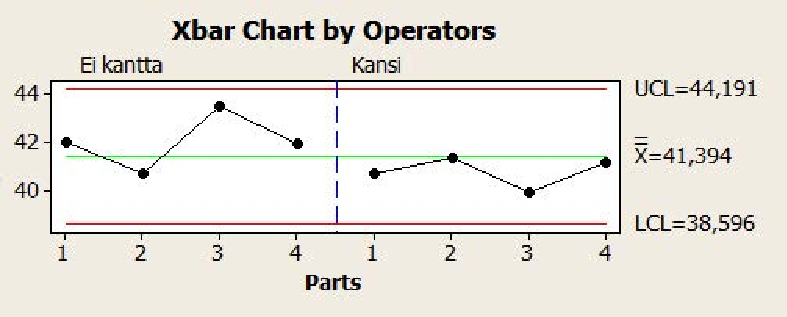
\includegraphics[width=\textwidth]{virtaus2xbar}
      \label{subfig:virtaus2xbar}}
    %\qquad                        % i) Ugly hack to get more horizontal space between figures
    %\hspace{0.05\textwidth}      % ii) Another ugly way to hack space
    % ~~                          % iii) Yet another...

    \subfigure[Toisen epätasaisen virtauksen kokeen R-chart-kuvaaja.]{
      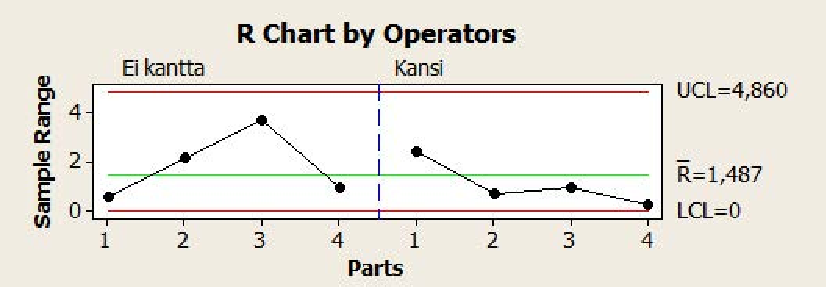
\includegraphics[width=\textwidth]{virtaus2rchart}
      \label{subfig:virtaus2rchart}}

    \subfigure[Toisen epätasaisen virtauksen kokeen tulokset, saman koekappaleen tulokset esitettynä rinnakkain.]{
      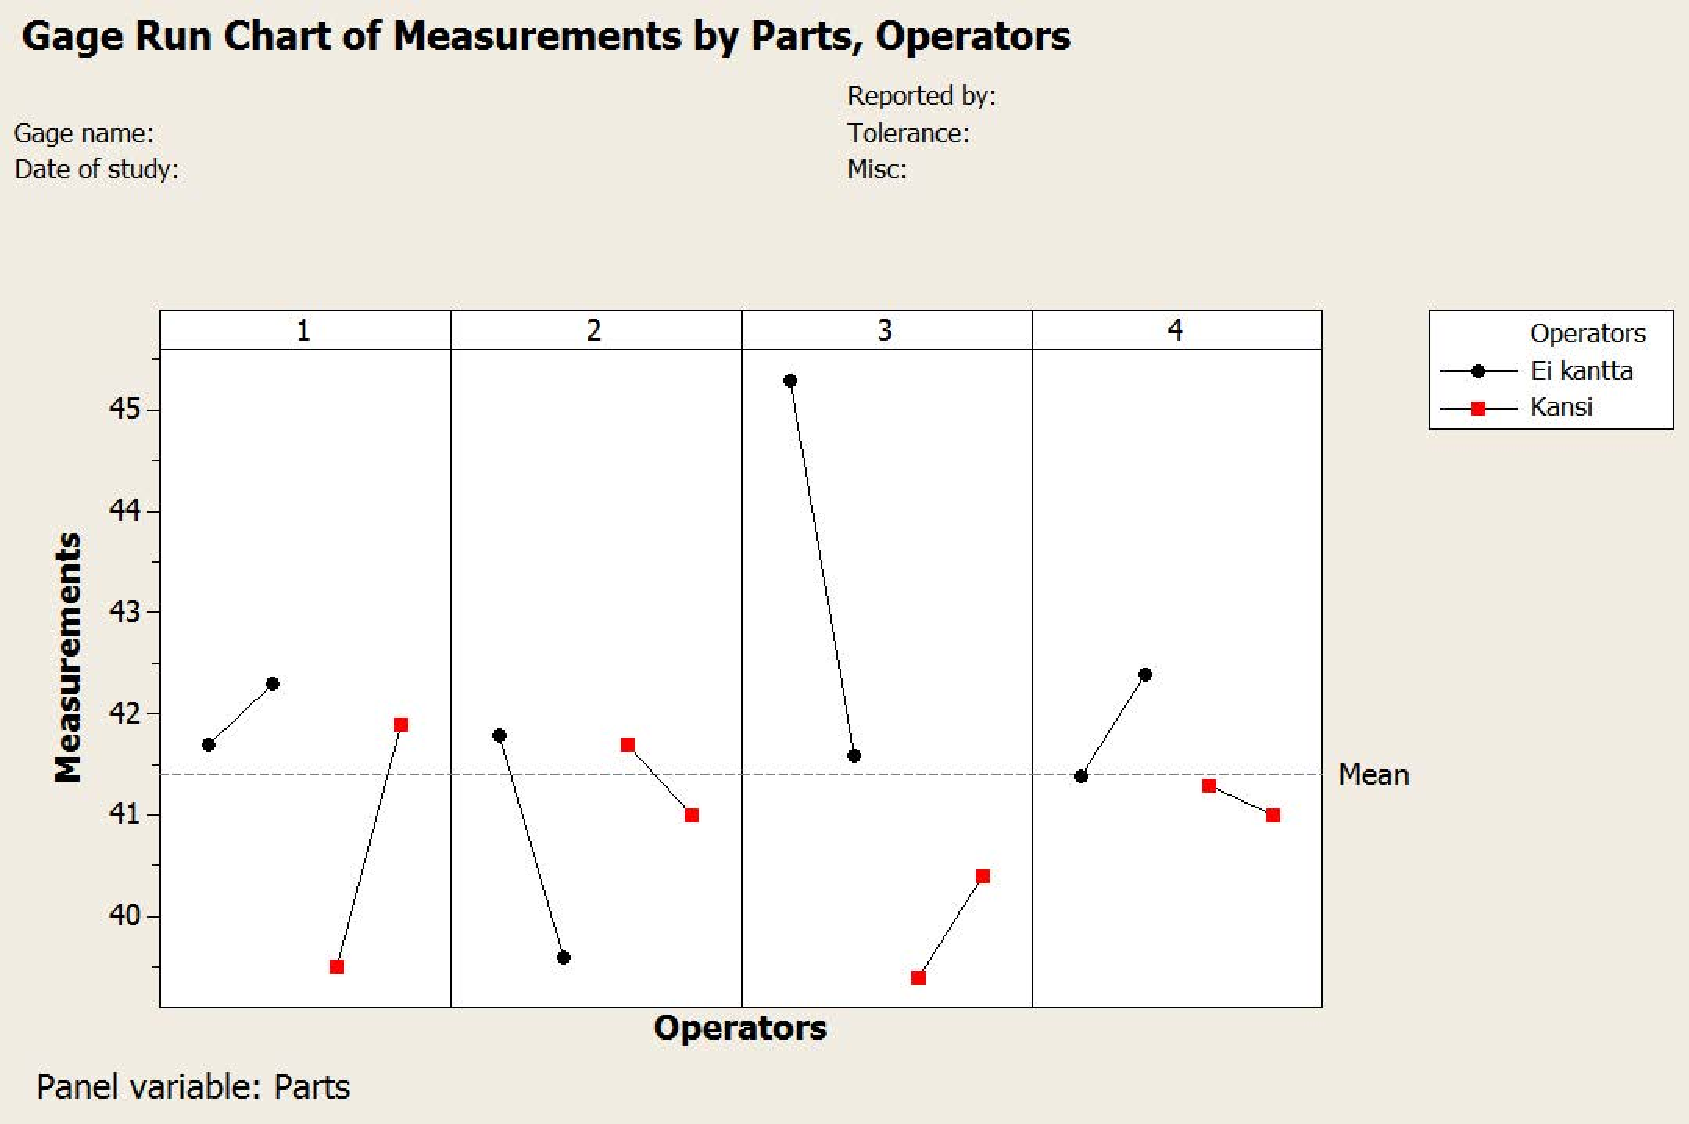
\includegraphics[width=\textwidth]{virtaus2rinnakkaiset}
      \label{subfig:virtaus2rinnakkaiset}}
    \caption[Toisen virtauskokeen tulokset]{Tulokset hiekan epätasaisen virtauksen tutkimuksesta kun koekappale on karbidipinnoitteinen.}
    % Optional shorter caption in brackets is used in Table of Figures
    % (tof).

    \label{fig:virtauskoe2}
  \end{center}
\end{figure*}


Tässä kokeessa ei löytynyt merkittävää eroa kannellisen ja kannettoman koeajon välillä.
On mahdollista että teräs on keraamia herkempää hiekkavirran turbulenssille tai että ”kansi – ei kantta” koejärjestely ei vastaa ”50 x 50 mm – 100 x 50 mm” koejärjestelyä. Joka tapauksessa tämä nimenomainen koetulos ei puolla hiekkavirran hallintaa kansikappaletta käyttämällä.

\section{Robustien parametrien suunnittelu}

Alunperin robustien parametrien suunnitteluun ajateltiin käytettäväksi
Taguchi-menetelmää. Projektin edetessä selventyi kuitenkin 2 syytä, joiden
vuoksi Taguchi-suunnitelma ei ollut sopiva tässä tapauksessa:

\begin{itemize}
  \item Taguchi–menetelmässä tekijöiden optimointiin käytetään
signaali-kohinasuhdetta, joka yhdistää koetuloksen keskiarvon ja varianssin. Tämä on tarpeetonta koska projektissa ei
yritetty tai haluttu säätää tulosten keskiarvoa millään tavalla.
  \item Taguchi-menetelmä on aktiivinen robustien parametrien suunnittelumenetelmä jossa kaikki ei-hallittavat tekijät pyritään ennen koetta tunnistamaan ja sitten kokeen aikana hallitsemaan. Tämä on hyvin toimivaa kun nämä häiriötekijät tunnistetaan tai tunnetaan jo etukäteen ja prosessi halutaan suojata niitä vastaan, mutta kumipyöräabraasiokokeessa
hajonnan syyt eivät olleet tarpeeksi hyvin tiedossa jotta aktiivista suunnittelua
oltaisi voitu toteuttaa.
\end{itemize}

Lopulta suunnitelmaksi valikoitui $2^k$ dispersiovaikutusten seulontakoe jossa kokeita toistetaan parametrien eri tasoilla ja toivotaan että vaihtelua esiintyy todellisuutta edustavalla tavalla. Toistojen määräksi valikoitui 4 koska 2
saman pinnoitteen näytekappaleeseen kumpaankin voidaan tehdä 2 koeajoa.

Koeajojen määrän pitämiseksi järkevänä oli tutkittavien parametrien määrä pidettävä pienenä. Lopulta päädyttiin 5 parametriin joiden vaikutus tuntui todennäköisimmältä:

\begin{itemize}
  \item Ajoaika
  \item Näytteen paine kumipyörää vasten
  \item Hiekan virtausmäärä aikayksikköä kohden
  \item Hiekan eli abrasiivin tyyppi
  \item Oliko edellisessä kokeessa käytetty hiekan virtausta ohjaava kansi paikallaan vai ei
\end{itemize}

Joka parametrille valittiin 2 tasoa, matala ja korkea. Ajoajalle valittiin 5 min ja 15 min, paineelle 0 kg punnus ja 1,5 kg punnus, hiekan virtaukselle 21 g/min ja 62 g/min, abrasiivityypille nilsiähiekka (-1) ja alumiinioksidi (1) ja kannelle ei kantta (-1) tai kansi paikoillaan (1). Hiekan virtausta oli tarkoitus tutkia myös suuremmilla arvoilla, mutta tarkoitukseen soveltuvia suuttimia ei löytynyt. Kumipyöräksi valittiin aiemmin hyväksi osoittautunut kumipyörä P2.

Varsinaista koesuunnitelmaa ei valittu valmiiden joukosta, vaan Minitab–makrolla luotiin D-optimaalinen suunnitelma. Etuna on että koeajojen määrä saatiin mahdollisimman pieneksi.

Koesuunnitelmasta muodostui kuvan \ref{fig:tarray} mukainen:
16 eri parametritasojen yhdistelmää, joista jokaisessa suoritettiin 4 koeajoa, yhteensä siis \(16\times 4 = 64\) koeajoa. 4 koetulokselle laskettiin keskiarvo ja keskihajonta.
Varianssin analysointiin on Minitabissa 2 arvointimenetelmää. Ensimmäinen, ”Least squares regression”, antaa kuvan \ref{subfig:pareto1} mukaisen Pareto–arvion parametrien vaikutuksista
ja ”Maximum likelihood” -menetelmä kuvan \ref{subfig:pareto2} mukaisen.
Tekijöiden vaikutusjärjestys, suurimmasta pienimpään, on molemmissa sama;
1 tekijän vaikutukset ovat ensimmäisinä ennen yhteisvaikutuksia.
Eniten vaikuttivat hiekan virtausmäärä ja paine koekappaleen ja kumipyörän välillä.
\todo{merkittävyysrajat}

\begin{figure}
  \begin{center}
    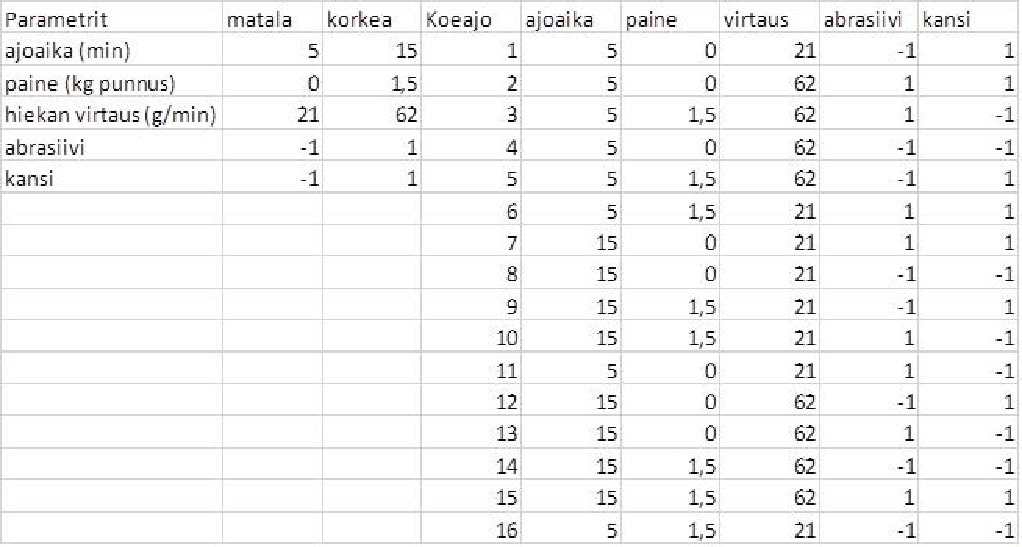
\includegraphics[width=1.0\textwidth]{tarray}
  \end{center}
  \caption[Robustien parametrien koesuunnitelma]{Robustien parametrien suunnittelukokeen koesuunnitelma.}
  % Optional shorter caption in brackets is used in Table of Figures
  % (tof).
  \label{fig:tarray}
\end{figure}


\begin{figure*}
  \begin{center}
    \subfigure[”Least squares regression” -menetelmän Pareto-kuvaaja.]{
      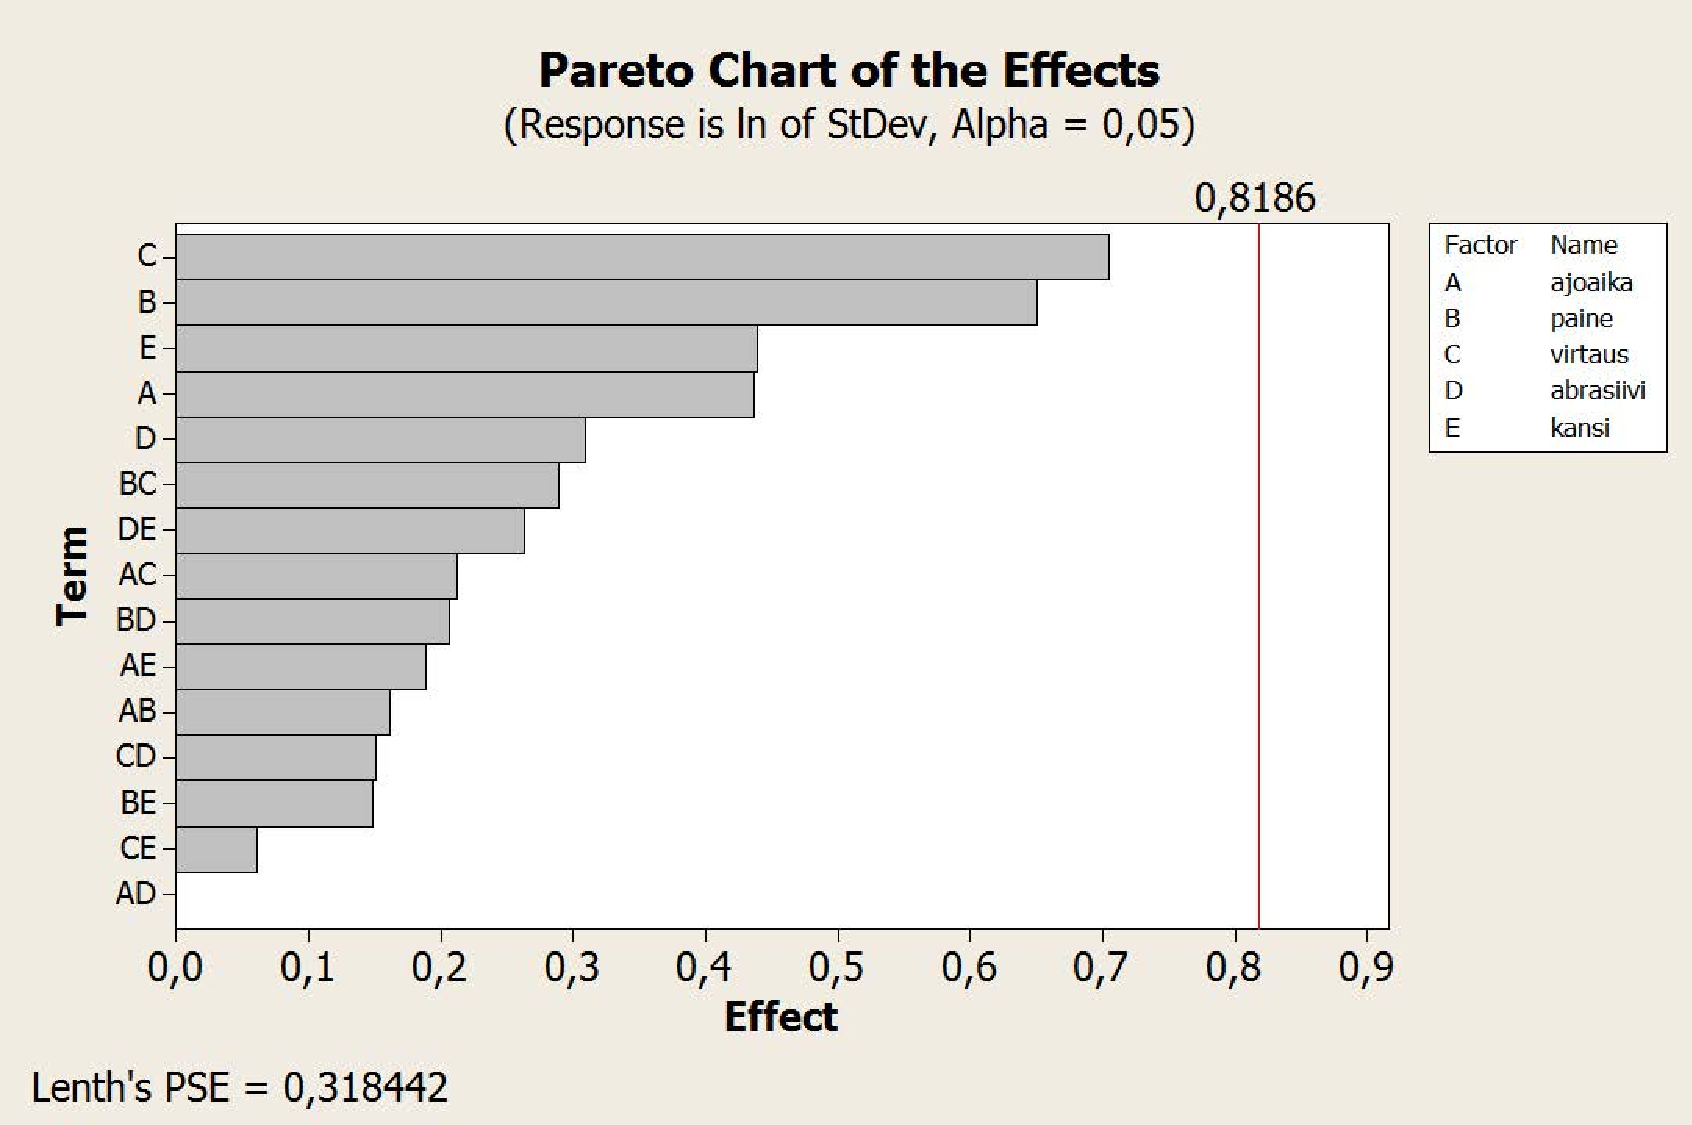
\includegraphics[width=\textwidth]{pareto1}
      \label{subfig:pareto1}}
    %\qquad                        % i) Ugly hack to get more horizontal space between figures
    %\hspace{0.05\textwidth}      % ii) Another ugly way to hack space
    % ~~                          % iii) Yet another...

    \subfigure[”Maximum likelihood” -menetelmän Pareto-kuvaaja.]{
      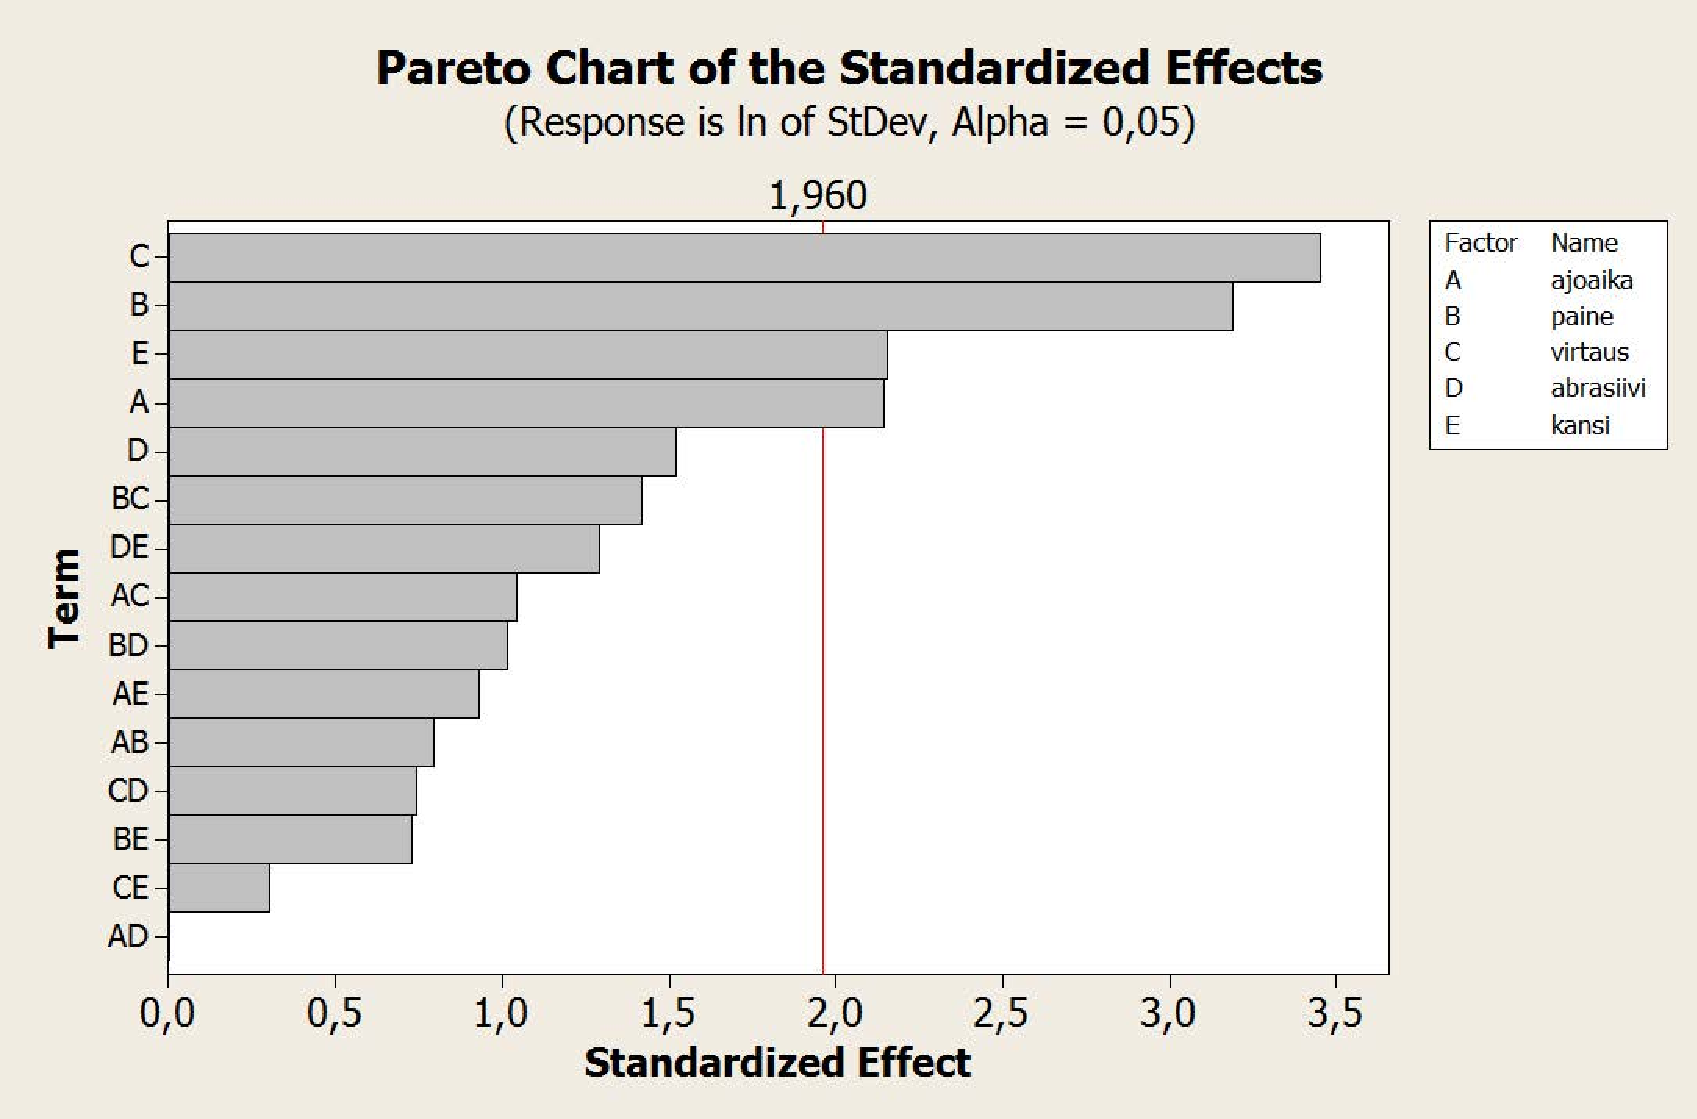
\includegraphics[width=\textwidth]{pareto2}
      \label{subfig:pareto2}}
    \caption[Robustien parametrien suunnittelukokeen tulokset]{Robustien parametrien suunnittelukokeen tulokset parametrien vaikutuksista.}
    % Optional shorter caption in brackets is used in Table of Figures
    % (tof).

    \label{fig:paretot}
  \end{center}
\end{figure*}





Jos kuitenkin vaikutusten pienuudesta huolimatta
jatketaan ja käytetään Minitabin optimointityökalua keskihajonnan minimointiin
saadaan tulos kuten kuvassa \ref{subfig:robusti1}.
Punaisella ylälaidassa näkyvät parhaiten keskihajontaa pienentävä parametrien arvojen yhdistelmä. Huomattiin kuitenkin että koska nähtävästi
optimointityökalu yrittää minimoida absoluuttisen keskihajonnan niin samalla se
pyrkii pienempiin ajoaikoihin vain koska silloin tuloksen keskiarvo ja sitä kautta myös keskihajonta pienenee, \em vaikka suhteellinen keskihajonta nousisikin. \em Päätettiin käyttää keskihajonnan sijasta yksikköä \em variaatiokerroin, \em kaavalla
\[v = \frac{s}{x} \times 100\> \%\]
missä \em s \em on keskihajonta ja \em x \em on keskiarvo.
Kirjallisuudesta paljastuikin myöhemmin variaatiokertoimen sisältyvän Taguchin suoritemitta-analyysiin vaikka Minitab ei tätä mainitsekaan \parencite{Steinberg1998,Kawamura2010,Wu2009}.
Variaatiokertoimet syötettiin Minitabiin, mutta koska Minitab ei ole asettanut mallia näihin arvoihin, vaan ainoastaan keskihajonnan arvoihin, ei variaatiokerrointa voida optimoida samalla työkalulla. Voidaan kuitenkin piirtää kuvan \ref{subfig:robusti2} mukainen vaikutuskuvaaja.
Tässä kuvassa ajoaika ja abrasiivi ovat aiempaan verrattuna päinvastoin, nyt pidemmällä ajoajalla ja käyttämällä alumiinioksidia saadaan paremmat tulokset. Ilman optimointityökalua ei voida kuitenkaan arvioida yhteisvaikutuksia.


\begin{figure*}
  \begin{center}
    \subfigure[Minitabin optimointityökalun tulokset keskihajonnan minimointiin.]{
      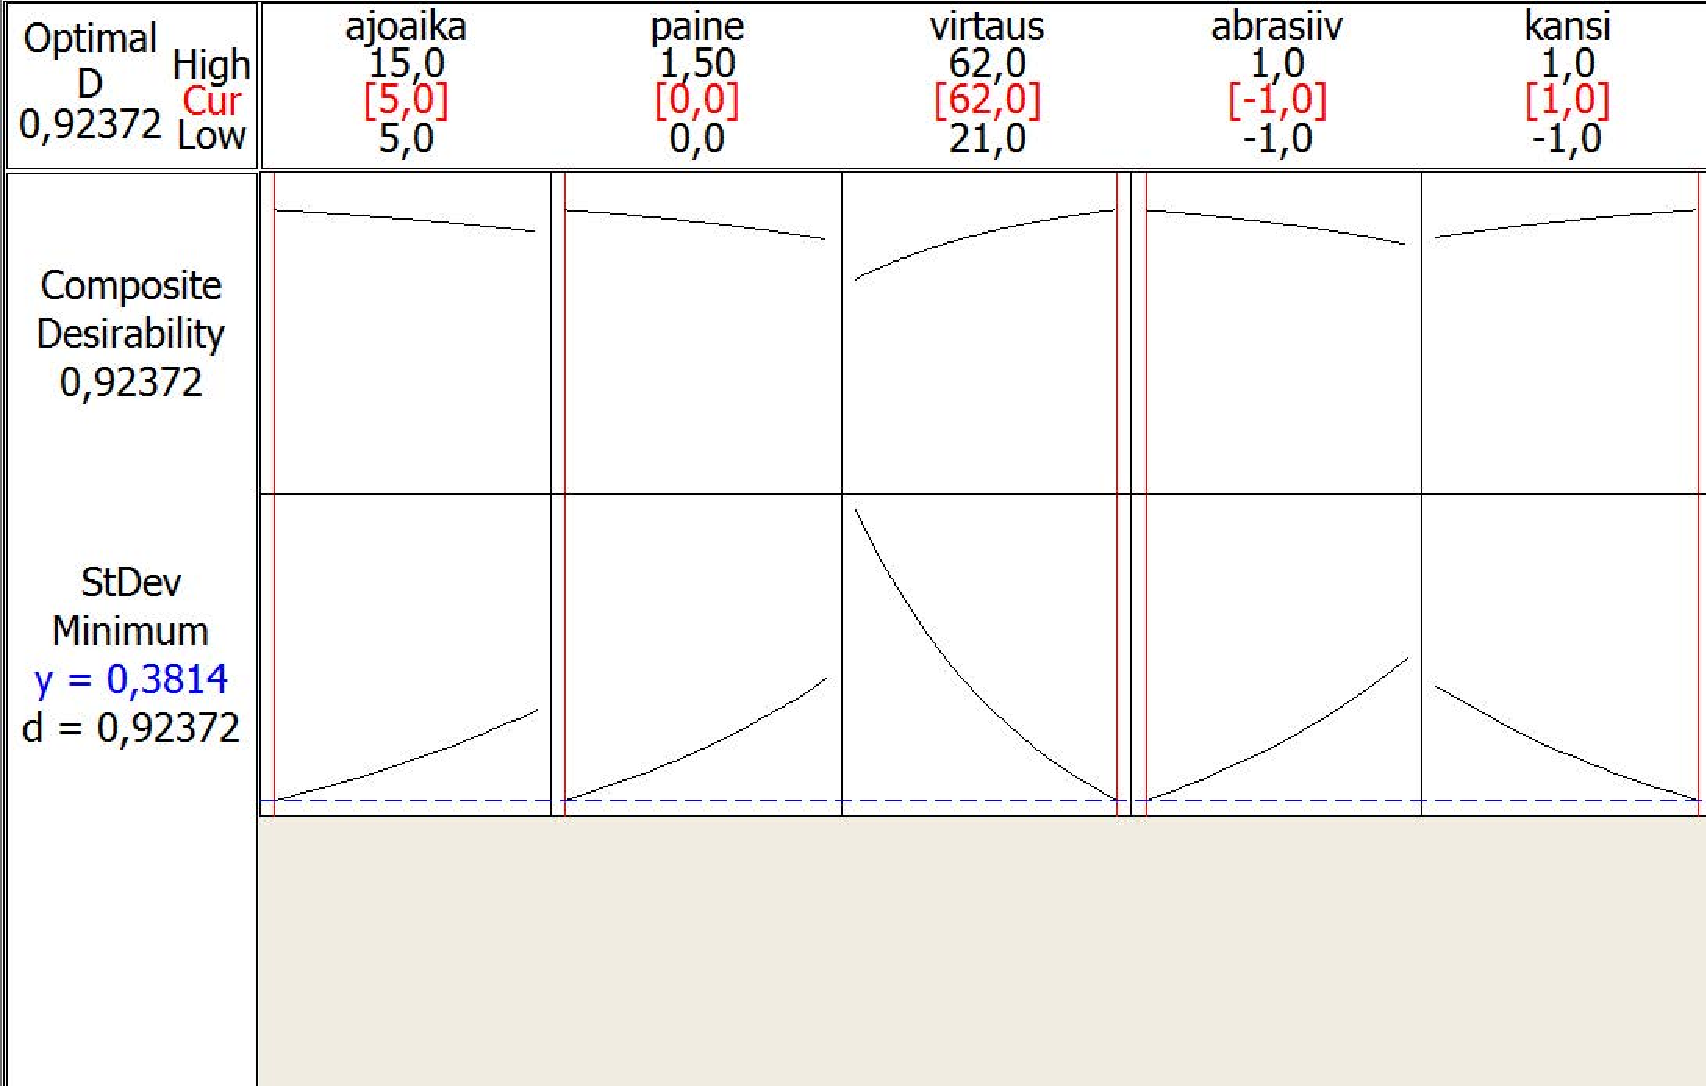
\includegraphics[width=\textwidth]{robusti1}
      \label{subfig:robusti1}}
    %\qquad                        % i) Ugly hack to get more horizontal space between figures
    %\hspace{0.05\textwidth}      % ii) Another ugly way to hack space
    % ~~                          % iii) Yet another...

    \subfigure[Minitabin vaikutuskuvaaja, tutkittujen parametrien vaikutus variaatiokertoimeen.]{
      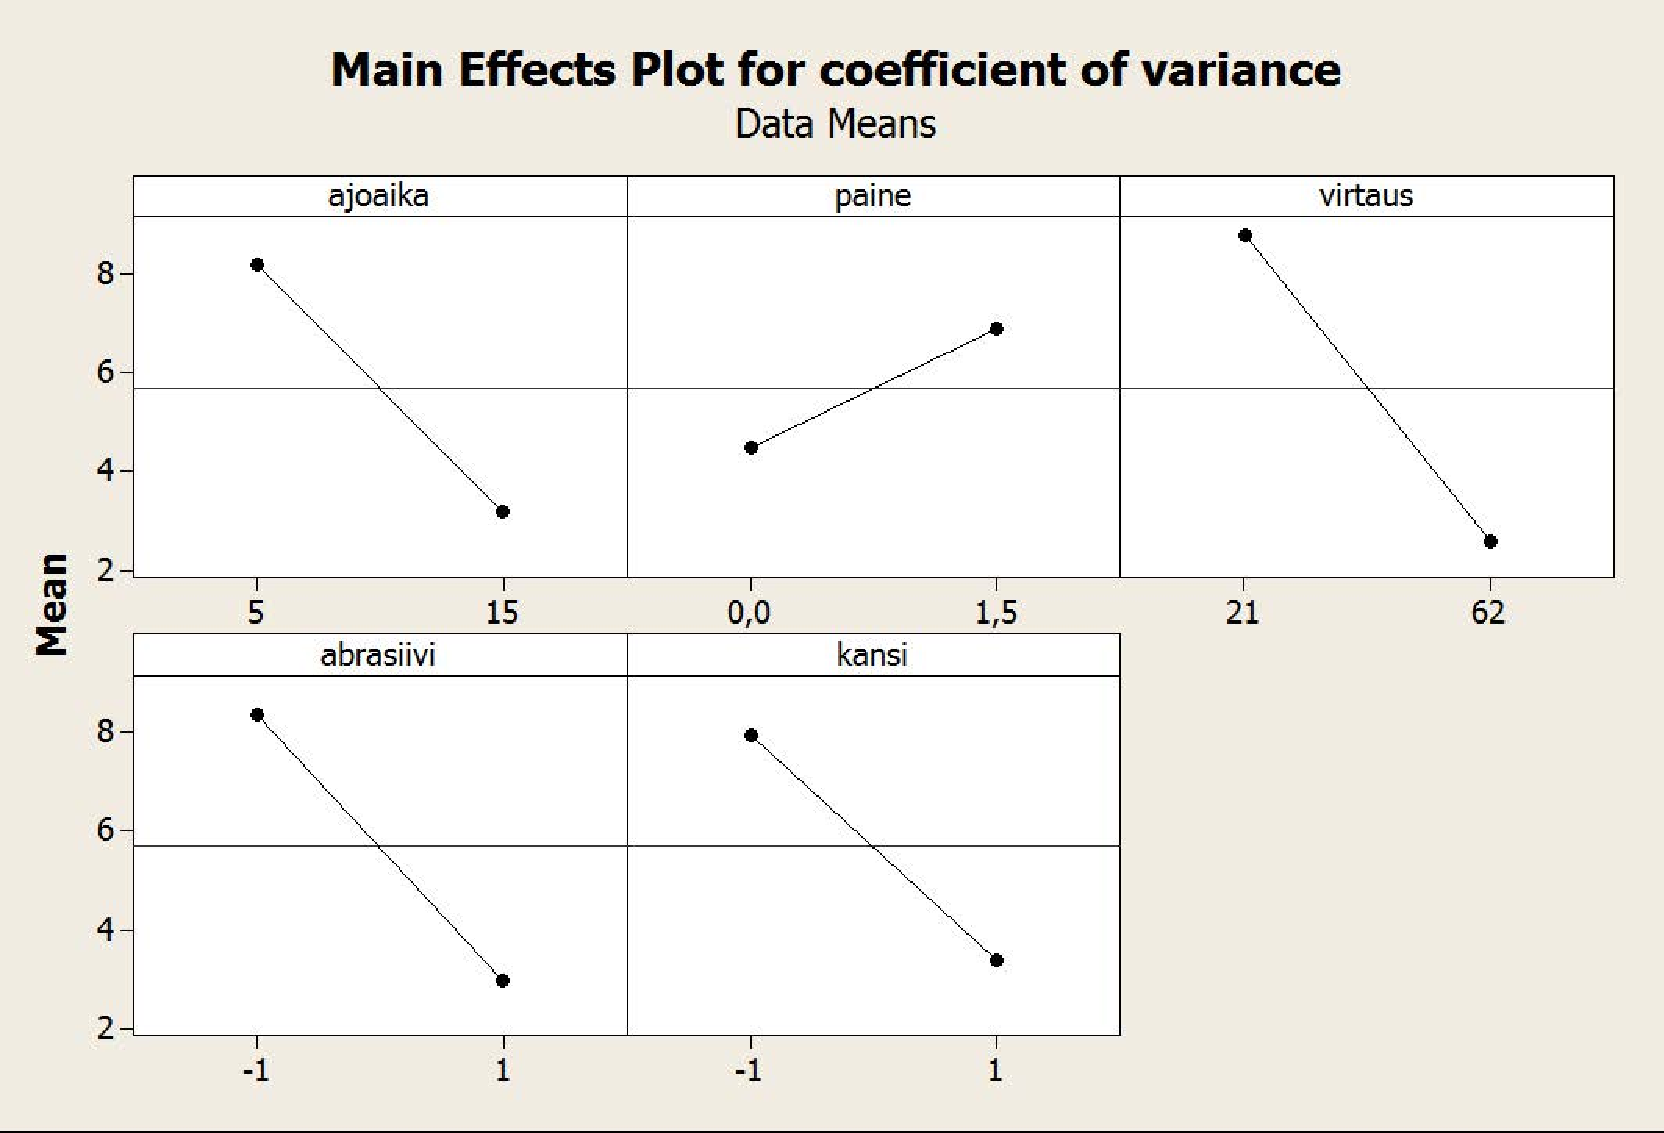
\includegraphics[width=\textwidth]{robusti2}
      \label{subfig:robusti2}}
    \caption[Robustien parametrien suunnittelukokeen tulokset kokeen optimointiin]{Robustien parametrien suunnittelukokeen tulokset parametrien säätämiseen.}
    % Optional shorter caption in brackets is used in Table of Figures
    % (tof).

    \label{fig:robustit}
  \end{center}
\end{figure*}





Kaiken kaikkiaan on hyvä muistaa että tässä robustien parametrien suunnittelussa tehtiin vain 4 toistokoetta jokaisella parametriarvojen yhdistelmällä.
Koska tekijöiden vaikutusta hajontaan mitataan nimenomaan näistä 4:stä toistokokeesta,
voi satunnainen kohina vaikuttaa tuloksiin paljon.
\todo{Ensimmäinen Pareto–kaavio myös arvioi kaikki vaikutukset merkityksettömiksi.}

\section{Kumipyörän P2 tyypin 1 mittajärjestelmäanalyysi}

Koska alussa täysin uutta kumipyörä P2:ta oli nyt käytetty kohtuullinen määrä, päätettiin sillä ajaa vielä muutama koe projektia varten valmistetulla näyte-erällä ja koota koko projektin aikana samalla pinnoitteella ko. pyörällä tehdyt koetulokset samaan taulukkoon, stabiiliuden ja pyörän kulumisen suhteen muutosten selvittämiseksi. Tulokset nähdään kuvassa \ref{fig:kp2grr}.
Tässä ”kokeessa” oli 16 koeajoa ja keskihajonta 2,71. Projektin ensimmäisessä kokeessa oli 20 koeajoa ja keskihajonta 1,78. Tässä viimeisessä kokeessa ero pienimmän ja suurimman koetuloksen välillä on jo suuri, n. 10 milligrammaa. Kuvaajan perusteella tulokset
muuttuvat
satunnaisemmiksi loppua kohden, tämän voisi kuvitella johtuvan kumipyörän kulumisesta lukuisissa vaihtelevissa kokeissa.


\begin{figure*}
  \begin{center}
    \subfigure[Kumipyörän P2 tyypin 1 mittajärjestelmäanalyysin tulos.]{
      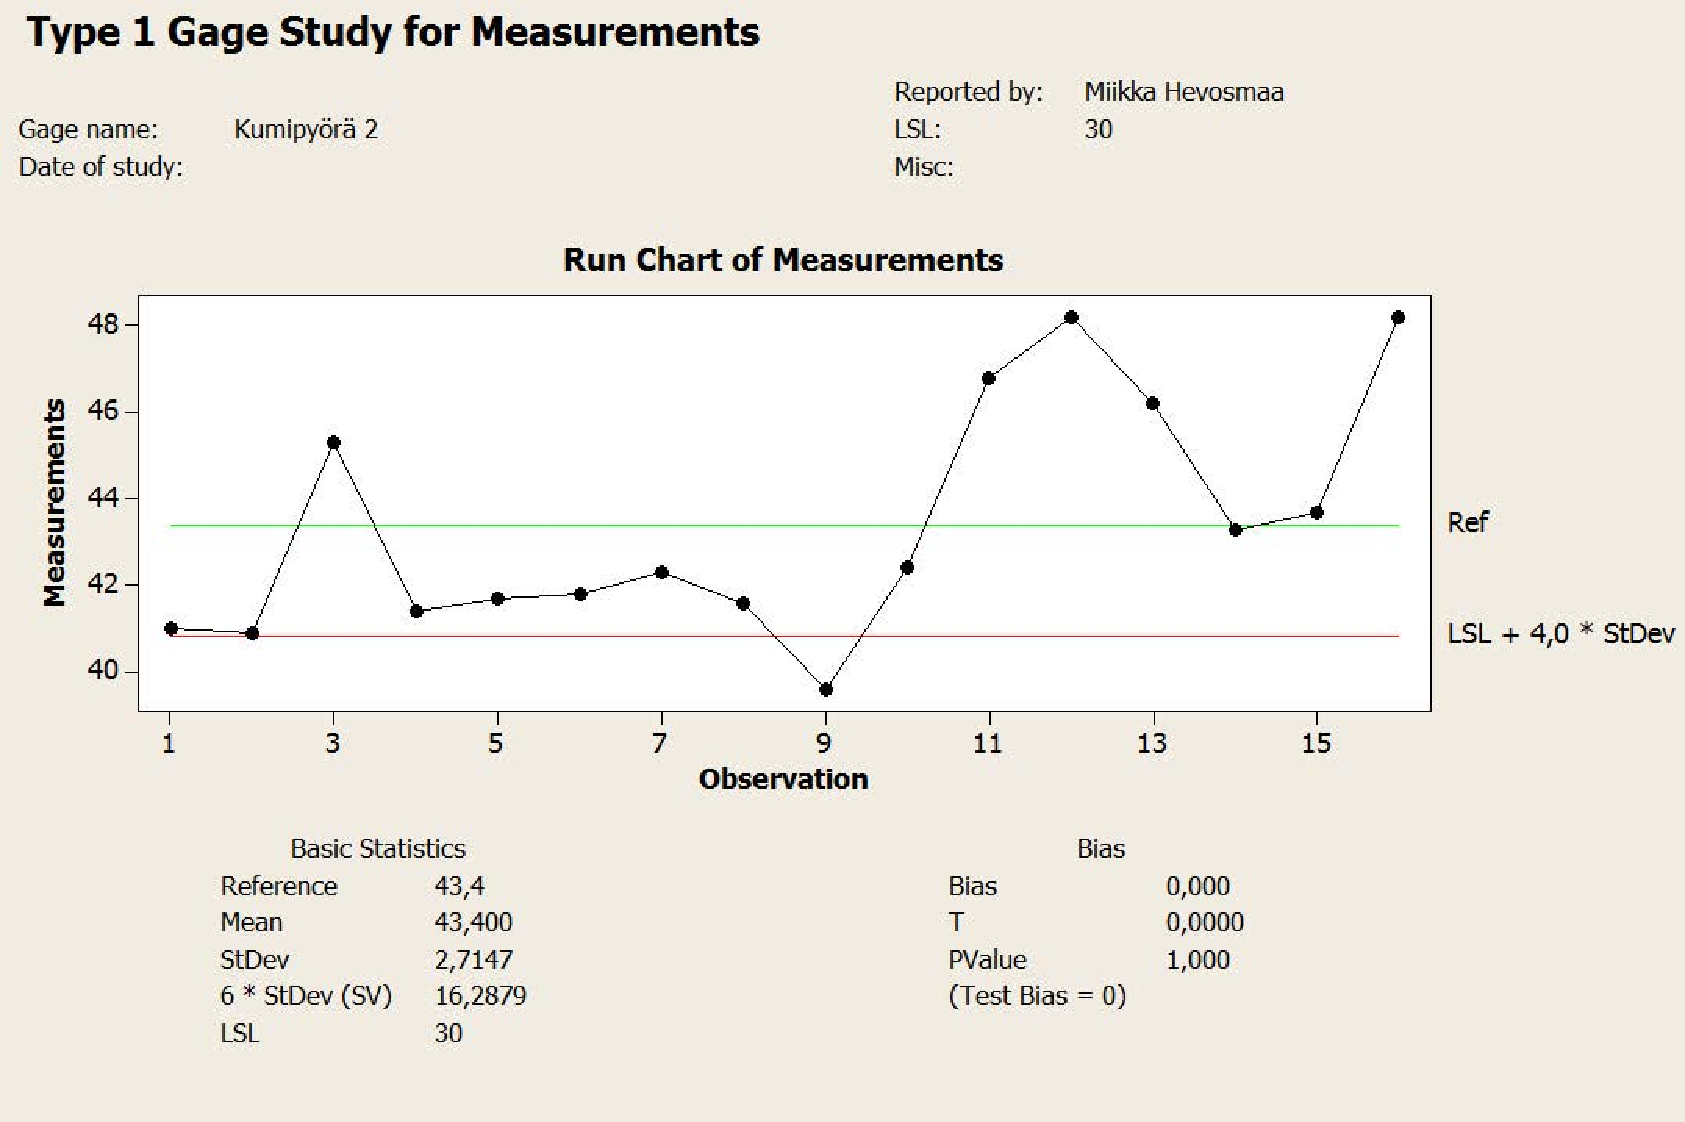
\includegraphics[width=\textwidth]{kp2grr1}
      \label{subfig:kp2grr1}}
    %\qquad                        % i) Ugly hack to get more horizontal space between figures
    %\hspace{0.05\textwidth}      % ii) Another ugly way to hack space
    % ~~                          % iii) Yet another...

    \subfigure[Kumipyörän P2 tyypin 1 mittajärjestelmäanalyysin tulos, saman koekappaleen tulokset rinnakkain.]{
      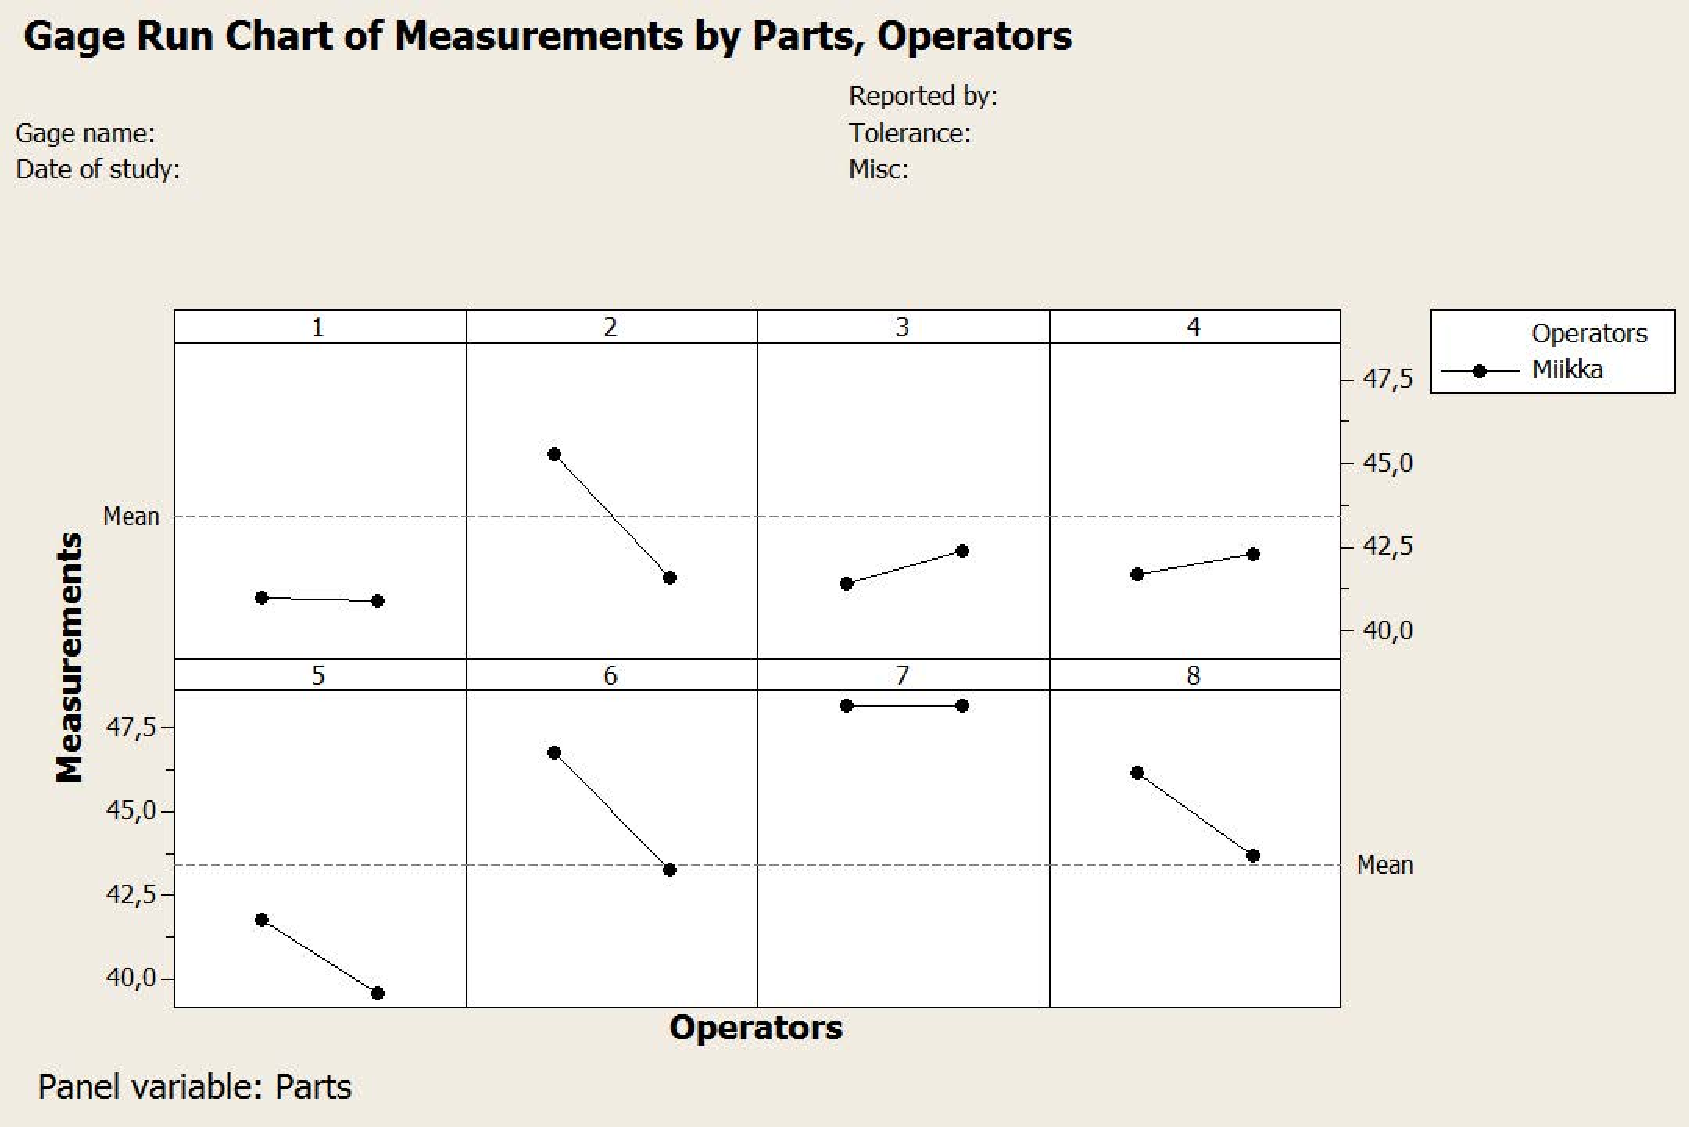
\includegraphics[width=\textwidth]{kp2grr2}
      \label{subfig:kp2grr2}}
    \caption[Kumipyörän P2 tyypin 1 mittajärjestelmäanalyysin tulokset]{Kumipyörän P2 tyypin 1 mittajärjestelmäanalyysin tulokset.}
    % Optional shorter caption in brackets is used in Table of Figures
    % (tof).

    \label{fig:kp2grr}
  \end{center}
\end{figure*}




%-------------------------------------------------------------------------------
\chapter{Conclusions}
\label{ch:concl}
%-------------------------------------------------------------------------------

\epigraph{The best time to plan an experiment is after you’ve done it}{R. A. Fisher}


Kaiken kaikkiaan mikään tutkituista tekijöitä ei vaikuttanut aiheuttavan
kovin merkittäviä disperiovaikutuksia. Tulos viittaa siihen että jos kumipyöräkoe
on antanut ajoittain poikkeavia tuloksia, on syy jossain muualla kuin tutkituissa
tekijöissä.


Robustien parametrien suunnitteluun käytettiin lopulta D-optimaalista
$2^k$-seulontakoetta



Kokeen aikana ei suuresta koeajojen määrästä huolimatta esiintynyt
suuresti odotetusta poikkeavia koetuloksia (yhtä teräsnäytettä lukuunottamatta).













%This template and the mathching Latex document class file together
%with general writing guidelines should help achieving a consistently
%formatted and clear documents. Similar template is also available for
%MS Word.

%Every writing and presentation must have a conclusion. This fact is
%here emphasized by having this short and rather artificial summary
%also in this template. A concise summary table is a good way for
%providing an overview of the most important points.















%-------------------------------------------------------------------------------
%\chapter{Referencing styles}
%\label{sec:ref_styles}
%-------------------------------------------------------------------------------

%Different referencing styles determine how you create 1) in-text
%citations and 2) the bibliography. Two common referencing styles are
%presented in this chapter:
%\begin{enumerate}
%\item	Numeric referencing (Vancouver system), such as [1],[2]...
%\item	Name-year system (Harvard system), such as (Weber 2001), (Kaunisto 2003)...
%\end{enumerate}

%A numeric reference is inserted in square brackets [~], whereasthe last
%name of the author and the year of publication are given in round
%brackets ().

%Both styles are acceptable, but the conventions for referencing vary
%between disciplines. You must pick one and use is consistently
%throughout your thesis. 

%\section{In-text citations}
%:
%In-text citations are placed within the body of the text as close to
%the actual citation as possible \parencite{rubberwheel}. The citation is generally placed
%within the sentence before the full stop. LaTeX has a command
%\texttt{\textbackslash cite} for this \parencite[p. 85]{oetiker14}. See the
%tex file for additional remarks for Harvard style citations \parencites {wang2010143}{alrefaie2010842}
%\parencite{alrefaie2010842}.
% The package Harvard has also additional commands, such as
% \citename{heinz06}, \citeyear{heinz06}, \citeasnoun{heinz06} and so
% on.
%
% Similarly the biblatex has a command \parencite{heinz06} to produce
% '(Heinz 2006)' instead of mere 'Heinz 2006'
%



%\begin{itemize}
%  \setlength{\itemsep}{-10pt} % Put these lines closer to each other
%  \small
%\item[] Weber argues that [1]. 
%\item[] Cattaneo et al. introduce in their study [2] a new...
%\item[] The result is ... [1, p. 23]. One must also note... [1, s. 33-36]
%\item[]
%\item[] In accordance with the presented theory ... (Weber 2001).
%\item[] It must especially be noted... (Cattaneo et al.).
%\item[] Weber (2001, p. 230) has stated...
%\item[]
%\item[] Based on literature in the field [1,3,5]...
%\item[] Based on literature in the field [1][3][5]...
%\item[] The topic has been widely studied [6-18]...
%\item[]
%\item[] ...existing literature (Weber 2001; Kaunisto 2003; Cattaneo et al. 2004) has...
%\end{itemize}


%\section{Bibliography}
%The entries must include all the details listed in Table~\ref{tab:bibl}.
%\begin{table}[!h]
%  \small
%  \begin{center}
%    \caption{Necessary bibliographic information.}
%    \label{tab:bibl}
%    \begin{tabular}{r l | r l }
%\hline 
%\textbf{\#}  
%   & \textbf{Numeric system}
%                       & \textbf{\#}  
%                                & \textbf{Name-year system}\\
%\hline
%\hline
%1. &	authors,	   & 1. & authors,  \\
%   &                       & 2. & (year in parentheses) \\
%2. &	title,             & 3.	& title,    \\
%3. &	publisher,         & 4.	& publisher,\\
%4. &	year of publication, &  &	 \\
%5. &	pages,             & 5.  & pages, \\
%6. &	URL, if applicable & 6.	& URL, if applicable    \\
%      \hline
%    \end{tabular}
%  \end{center}
%\end{table}


%Formatting examples of an journal article in bibliography are provided
%below, first in the numeric style and then the name-year style.

% Define columns widths to get text wrapped
%\begin{tabular}{p{1cm}p{12cm}}
%\small
%[100] & K. Keutzer, A.R. Newton, J.M. Rabaey,
%A. Sangiovanni-Vincentelli, System-level design: orthogonalization of
%concerns and platform-based design, IEEE Transactions on
%Computer-Aided Design of Integrated Circuits and Systems, vol.19,
%no.12, Dec 2000, pp.1523-1543.\\
%\end{tabular}

%\begin{tabular}{p{13cm}}
%\small
%Keutzer, K., Newton, A.R., Rabaey, J.M. \& Sangiovanni-Vincentelli
%A. (2000). System-level design: orthogonalization of concerns and
%platform-based design. IEEE Transactions on Computer-Aided Design of
%Integrated Circuits and Systems. Vol.19(12), s.1523-1543. \\
%\end{tabular}

%Your references are listed at the end of your thesis in alphabetical
%order based on the first author's last name. If the author is unknown,
%alphabetize the source using the corporate author or title.


%LaTeX has two ways for making reference list
%\begin{enumerate}
%\item using automated Bibtex tool
%\item manually
%\end{enumerate}

%The tex source of this document has both versions, and the other is in
%comments. Bibtex\footnote{\url{http://ctan.org/pkg/bibtex}} formats the
%reference list according to a setup file, which is usually provided by
%academic journals. You need to write the basic information into
%\texttt{.bib} file. Citations in your tex file at looked up by bibtex
%and it produces the list of references automatically.

%\subsection{Header at 3rd level}
%\label{sec:3rd}
%Some text...

%\subsection{Another header at 3rd level}
%\label{sec:3rd_partner}

%Section~\ref{sec:3rd} cannot appear alone, but needs some company
%(i.e.~\ref{sec:3rd_partner}).

%\subsubsection{Avoid 4th level headers}
%Luckliy they are not numbered in this LaTeX template


% \paragraph{Paragraph}
% Fifth level header
% Empty line is a paragraph separator in LaTeX.





%-------------------------------------------------------------------------------
% The bibliography, i.e the list of references (3 options available)
%-------------------------------------------------------------------------------
\newpage

%\renewcommand{\bibname}{Bibliography}     % Otherwise bilingual babel uses Finnish ``Kirjallisutta''. Strange...
\renewcommand{\bibname}{Lähteet}         % Set Finnish header, remove this if using English
\addcontentsline{toc}{chapter}{Lähteet}  % Include this in TOC
%\addcontentsline{toc}{chapter}{\bibname}  % Include this in TOC


%
% Option1: Write the bibliographic information into .bib file
% (e.g. thesis_refs.bib) and use bibtex tool to do the formatting.
%

% You must execute: pdflatex d_tyo.tex; bibtex d_tyo; pdflatex.tex
% First command creates the cross-refeerence file .aux for bibtex and
% last combines the bibtex output to the rest.  Many styles are
% available, see e.g. at
% http://www.ctan.org/tex-archive/biblio/bibtex/base
% http://www.reed.edu/cis/help/latex/bibtexstyles.html

% 1a) Numeric style:
%\bibliographystyle{IEEEtranS}   % the IEEE's sorted numeric style
% List is sorted first by author if present. If not, then by editor,
% organization, title, and last by key.
% http://mirrors.ctan.org/macros/latex/contrib/IEEEtran/bibtex/IEEEtran_bst_HOWTO.pdf

% 1b) Author-year style:
% see http://www.ctan.org/tex-archive/macros/latex/contrib/harvard/


%\bibliography{thesis_refs}    % Insert {author,title,year...} info of your reference
%\markboth{\bibname}{\bibname} % Set page header


%
% Option2: Write all information directly into this tex file. They
% appear as written here. Note that these is no check if you actually
% cite these.
%

%\begin{thebibliography}{99}        % Up to 99 items
%\markboth{\bibname}{}              % Set page header

% 2a) Numerical refs

%\bibitem{heinz06} C. Heinz, B. Moses, J. Hoffmann, listings - Typeset
%  source code listings using LaTeX, Comprehensive TeX Archive Network
%  (CTAN), 2006. Available: \url{http://www.ctan.org/pkg/listings}

%\bibitem{latex13} LaTeX, Wikibooks, March 2013, 706 pages.  Available:
%  \url{http://en.wikibooks.org/wiki/LaTeX/}

%\bibitem{mittelbach04} F. Mittelbach, M. Goossens, J. Braams,
%  D. Carlisle, C. Rowley, The Latex Companion, 2nd ed., Boston,
%  Addison-Wesley, 2004, 1120 s.

%\bibitem{oetiker14} T. Oetiker, H. Partl, I. Hyna, E. Schlegl, The Not
%  So Short Introduction to LATEX2$\epsilon$ - Or LATEX2$\epsilon$ in
%  157 minutes, Version 5.03, 2014, 171 p. Available:
%  \url{http://www.ctan.org/tex-archive/info/lshort/english/}

%\bibitem{ruohonen09} K. Ruohonen, Matemaattisen tekstin
%  kirjoittaminen, Tampereen teknillinen yliopisto, 2009, 7
%  s. Available: \url{http://math.tut.fi/~ruohonen/D-tyo-ohje.pdf}

%\bibitem{salminen09} E. Salminen, Practical advice for writing
%  publications, course material, TKT-9617 Scientific Publishing,
%  Tampere University of Technology, Nov 2009 (updated Aug 2012), 101
%  p. Available:
%  \url{http://www.cs.tut.fi/~ege/Misc/salminen_figures_styles_v15.pdf}

%\bibitem{thesisguide13} Thesis Writing Guide in English, Tampere
%  University of Technology guidelines, Tampere, 2013. Available:
%  \url{https://www.tut.fi/pop} > Study info > Master's thesis > MSc
%  thesis guidelines

%
% 2b) Author-year style
%
%% Harvard-like referencing needs adding \usepackage{harvard}
%% to the preamble and using \harvarditems instead of \bibitem
%\harvarditem{Heinz, Moses and Hoffmann}{2006}{heinz06}
% C. Heinz, B. Moses, J. Hoffmann, listings - Typeset source code
% listings using LaTeX, Comprehensive TeX Archive Network (CTAN),
% 2006. Available: \url{http://www.ctan.org/pkg/listings}
% http://mirrors.ctan.org/macros/latex/contrib/harvard/harvard.pdf

% \end{thebibliography}


%
% Option 3: Use newer package biblatex .Check that your environment
% has it installed.
%
% http://www.ctan.org/pkg/biblatex
%

\printbibliography                  % a) heading in English
%\printbibliography[title=Lähteet]   % b) heading in Finnish
%\addtocontents{toc}{%               % b) add Finnish heading to table of contents
% \protect\noindent Lähteet\protect\par
%} 






\end{document}

%sagemathcloud={"latex_command":"pdflatex -synctex=1 -interact=nonstopmode 'd_tyo.tex'"}